\documentclass{FastFyp}
\setlength{\headheight}{14pt}

% tabularx, colortbl, float not in class -- load here
\usepackage{tabularx}
\usepackage{colortbl}
\usepackage{float}
\newcolumntype{P}[1]{>{\raggedright\arraybackslash}p{#1}}
% booktabs and array already loaded by FastFyp.cls -- no need to reload
\definecolor{tableheader}{RGB}{225, 235, 245}
\definecolor{rowalt}{RGB}{247, 250, 253}

\setcounter{tocdepth}{2}
\setcounter{secnumdepth}{3}

% Centre diagrams on float-only pages and avoid stretching short text pages.
\raggedbottom
\makeatletter
\setlength{\@fptop}{0pt plus 1fil}
\setlength{\@fpbot}{0pt plus 1fil}
\makeatother
\begin{document}

\newcommand{\supervisor}{Dr.~Zeeshan Ali Rana}
\newcommand{\university}{National University of Computer and Emerging Sciences, Lahore}
\newcommand{\fyptitle}{AetherFlow}
\newcommand{\degree}{BS}
\newcommand{\Studentone}{Muhammad Abdul Raheem Khan \quad 23L-0588 \quad BS(CS)} 
\newcommand{\Studenttwo}{Muhammad Umar Shoaib Khokhar \quad 23L-0934 \quad BS(CS)}
\newcommand{\Studentthree}{Ahmad Rasheed \quad 23L-0786 \quad BS(CS)}
\date{October 21, 2026}
\renewcommand{\contentsname}{Table of Contents}

\hypersetup{pageanchor=false}
\makeatletter
    \begin{titlepage}
        
\includegraphics[width=0.2\linewidth]{Figures/nulogo.png}\hfill
        
\includegraphics[width=0.2\linewidth]{Figures/fast.png}\\
        \begin{center} 
            {\large\bfseries \university}\\[7ex]
            
\includegraphics[width=0.4\linewidth]{Figures/fastlogo.png}\\[8ex]
            {\huge \bfseries  \fyptitle }\\[10ex] 
            {\Studentone}\\{\Studenttwo}\\{\Studentthree}\\[4ex] 
            {Supervisor: \supervisor} \\ [10ex]
            {Final Year Project}\\
            {\large October 21, 2026}
        \end{center}
    \end{titlepage}    
\makeatother
\frontmatter

\newpage \thispagestyle{empty} \mbox{} \newpage %Aatira

\hypersetup{pageanchor=true}

\pagestyle{empty}  %Aatira
\section*{\begin{center}{Anti-Plagiarism Declaration} \end{center}} %Aatira
This is to declare that the above publication was produced under the:
\begin{flushleft}
\bf Title: \fyptitle
\end{flushleft}

is the sole contribution of the author(s), and no part hereof has been reproduced as it is the basis (cut and paste) that can be considered Plagiarism. All referenced parts have been used to argue the idea and cited properly. I/We will be responsible and liable for any consequence if a violation of this declaration is determined.
\\[4ex]
Date: October 21, 2026

\begin{flushright}
Name: Muhammad Abdul Raheem Khan (23L-0588)
\\[3ex]
Signature: \makebox[2.8cm][l]{\makebox[0pt][l]{..........................}\makebox[2.8cm][c]{\raisebox{-0.15cm}[0pt][0pt]{
\includegraphics[width=2.6cm,height=0.9cm,keepaspectratio]{Figures/signatures/raheem.png}}}}
\\[6ex]
Name: Muhammad Umar Shoaib Khokhar (23L-0934)
\\[3ex]
Signature: \makebox[2.8cm][l]{\makebox[0pt][l]{..........................}\makebox[2.8cm][c]{\raisebox{-0.2cm}[0pt][0pt]{
\includegraphics[width=2.4cm,height=1cm,keepaspectratio]{Figures/signatures/umar.png}}}}
\\[6ex]
Name: Ahmad Rasheed (23L-0786)
\\[3ex]
Signature: \makebox[2.8cm][l]{\makebox[0pt][l]{..........................}\makebox[2.8cm][c]{\raisebox{-0.2cm}[0pt][0pt]{
\includegraphics[width=2.2cm,height=1.1cm,keepaspectratio]{Figures/signatures/ahmad.png}}}}

\end{flushright} 

\vspace{3.5 cm} %Aatira
 
\hrule %Aatira

\section*{Author's Declaration}
This states Authors' declaration that the work presented in the report is their own, and has not been submitted/presented previously to any other institution or organization.
\pagebreak

\section*{Abstract}

Organizations deploying LLMs need to trade-off between the cost of inference, latency, quality of responses, and data privacy. This document presents \textbf{AetherFlow}: A Privacy Aware, Multi-Objective LLM Gateway between Clients and Language Models. AetherFlow performs four major tasks for each request - Privacy Screening, Semantic Caching with Answer Validation, Pre-Inference Quality Assessment, and Heterogeneous Inference across local and cloud LLMs. Execution Policy Engine chooses the target of execution by maximizing the utilities of quality, cost, and latency with the constraint of privacy. The Visual Studio Code extension is also provided for reference.
\pagebreak

\section*{Executive Summary}

Today, Large Language Models (LLMs) are employed in code assistants, chatbots, and enterprise search, and enterprises which use LLMs on a large scale should be able to satisfy four contradicting requirements, which are cost, latency, quality, and privacy. While the cloud-based frontier models are the most advanced in terms of quality, they are costly and introduce latency, and sensitive prompts might leak to the external provider. On the other hand, while the open-weight models that are stored locally cost less, they might lack quality, especially when dealing with sophisticated prompts. The prompts which are sensitive (that is, which include personal identifiable information and/or credentials) represent an additional constraint, since such prompts cannot be passed to a third-party.

The AetherFlow is a multi-objective LLM gateway focused on providing solutions to these challenges at once. It is designed as an asynchronous FastAPI proxy placed in-between client applications and language-model backends; in turn, the proxy decides for every query whether the answer should be retrieved from cache, local model, or cloud API. Every request goes through four stages of processing. At the Privacy Analyzer stage, the prompt is scanned using Microsoft Presidio, masked by personally identifiable information, and the confidential request is kept on local models. Semantic cache powered by Qdrant finds the similar previous query and checks the candidate answer, thus reducing the chance of false-positive cache hits. When it comes to requests routed further, fine-tuned DistilDeBERTa-v3-small classifier predicts, without any models running yet, how well each candidate is going to perform in answering the request. Finally, the request gets routed to a heterogeneous set of backends: local models Qwen3-8B and Llama-3.1-8B-Instruct provided via vLLM or Ollama and cloud models GPT and Gemini using API keys provided by the user.

Routing is decided by the Execution Policy Engine, which weighs in the quality estimate along with cost and latency, and chooses the backend that maximizes a weighted utility function. Privacy is a hard constraint rather than a weighted component, meaning that any backends that would infringe on it are stripped out before considering any trade-offs. The weights can be customized by the administrator, meaning that the trade-off between quality, cost, and latency can be customized per installation.

For showcasing the gateway in a real-world scenario, the project has a Visual Studio Code extension as the reference client. This extension allows for a chat pane and code-aware operations performed on the selected code – namely, explaining, fixing, refactoring, and generating tests. At the same time, all model interactions, privacy filtering, and routing are carried out through the gateway. An observability dashboard is offered along with the client to present savings on costs, latency, cache hit rate, and model query distribution.

This report encompasses all aspects of the project life cycle. It discusses the project’s vision and the background of research related to the problem. This is followed by the definition of software requirements, the proposed methodology, and the description of the software high-level and low-level design. Evaluation and benchmarking directions are formulated using the MMLU, GSM8K, HumanEval, and MT-Bench datasets.
\pagebreak

\pagestyle{fancy} %Aatira
\tableofcontents

\pagebreak
\listoffigures	% comment this if there are no figures
\addcontentsline{toc}{chapter}{List of Figures}
\pagebreak
\listoftables % comment this if there are no tables
\addcontentsline{toc}{chapter}{List of Tables}

\mainmatter

\chapter{Introduction}
\label{ch:introduction}

LLMs can be used to develop programming assistants, chatbots, and enterprise search systems. The Cloud API and locally installed open-weight models possess their own set of abilities, costs, and latency. Even a top-notch cloud model might make an error, while a local one could require substantial computation. Enterprises need to make decisions based on measurements for incoming requests.

The issue of data privacy is a separate limitation. There is no blanket prohibition on processing of data by a third party under the GDPR and HIPAA regulations, legal grounds, safeguards, processor requirements, and business associate provisions must be considered \cite{ref:GDPR,ref:HIPAA}. AetherFlow does not provide any guarantees on being legally compliant. They propose a technical realization of the list of destination selected by the administrators, which also includes processing of restricted data locally only.

AetherFlow inserts a gateway between client applications and language model backends. The process of the latter involves four steps: privacy screening, semantic caching, quality estimate prior to inference, and the execution policy with heterogeneous inference. The utility function is considering only destinations that passed the privacy screening step.
%--------------------------------------------------------------
\section{Purpose of this Document}
\label{sec:purpose}

This document attempts to provide a thorough and systematic description of AetherFlow for its audience, which includes both developers and users. In this document, the vision, objectives, and requirements of this project will be discussed, which would form the basis for the design and evaluation of a privacy-based multi-objective gateway for enterprise large language models (LLMs) routing. The four phases of the pipeline such as privacy filtering, semantic caching, pre-inference quality estimation, and heterogeneous inference execution policy have been described in detail.
%--------------------------------------------------------------
%--------------------------------------------------------------
\section{Intended Audience}
\label{sec:audience}

This report is meant to attract people with varied interests in AetherFlow, and each person may find some specific chapters interesting to his/her respective roles. This report is targeted towards the following readers:

\begin{enumerate}
    \item Project supervisors and FYP evaluation boards, who can evaluate the contribution of the project from problem definition, methodological approach, experiment setup, and engineering perspective.
    \item Software architects and DevOps engineers, who can come up with the deployment strategy of AetherFlow from gateway architecture, asynchronous proxy design, abstraction of serving locally and in cloud, and technology stack (FastAPI, Qdrant, Presidio, vLLM, and Ollama).
    \item Information security and compliance experts, who can evaluate the privacy screening pipeline, PII obfuscation, local-only execution of sensitive inputs, and auditing process.
\end{enumerate}

Basic familiarity with large language models and web services architecture is presumed by the readers.

%--------------------------------------------------------------
\section{Definitions, Acronyms, and Abbreviations}
\label{sec:definitions}

\begin{flushleft}
\setlength{\parindent}{0pt}
\setlength{\parskip}{0pt}
\textbf{AetherFlow:} The privacy-centric, multi-objective LLM gateway proposed in this project. \\
\textbf{LLM:} Large Language Model. \\
\textbf{API:} Application Programming Interface. \\
\textbf{PII:} Personally Identifiable Information. \\
\textbf{NER:} Named Entity Recognition. \\
\textbf{GDPR:} General Data Protection Regulation. \\
\textbf{HIPAA:} Health Insurance Portability and Accountability Act. \\
\textbf{ANN:} Approximate Nearest Neighbor. \\
\textbf{HNSW:} Hierarchical Navigable Small World. \\
\textbf{SSE:} Server-Sent Events. \\
\textbf{BYOK:} Bring Your Own Key. \\
\textbf{SRS:} Software Requirement Specification.
\end{flushleft}

%--------------------------------------------------------------
%--------------------------------------------------------------
\section{Conclusion}
\label{sec:ch1-conclusion}

This document presents AetherFlow with a universal threshold for confidentiality controls and resource-aware model selection. This document outlines the problem, reviews relevant literature, and identifies requirements and an evaluatable design. This report makes the distinction between the current client prototype versus the yet-to-be-implemented gateway function.
\chapter{Project Vision}
\label{ch:vision}

This chapter elaborates on the vision of AetherFlow. It contains the description of the problem domain, the problem which is being solved, as well as the project goals, scope, constraints, and the business case. The beneficiaries of the gateway are also provided in this chapter. The justification of the necessity to create a privacy-preserving multi-objective LLM gateway is provided in this chapter.
%--------------------------------------------------------------
\section{Problem Domain Overview}
\label{sec:domain}

LLMs are currently used in code assistants, chatbots, and enterprise search applications. When it comes to enterprise applications, these use cases do not typically rely on just one model but rather rely on a mixture of highly capable commercial cloud models and light open models which run on-premises and have differing characteristics in regard to cost, performance, quality, and data processing.

In the absence of an intermediary layer, the client application would be connected to just one provider. This implies that the company has to make a choice between routing all its traffic to its best cloud models and facing higher costs, latency, and exposure of prompts to external providers. On the other hand, it could restrict its users from using any other model but the one running on-premises and thus maintain the privacy of its data while losing quality of the results in difficult cases.

%--------------------------------------------------------------
\section{Problem Statement}
\label{sec:problem-statement}

When organizations deploy large-scale LLMs, they must choose for each request which backend should process it. This choice should consider output quality, monetary cost, and response latency while not forwarding the identified sensitive input to an external party.

Let us formally introduce $q$ as an incoming request and let $M=\{m_1,\ldots, m_K\}$ be the set of available backends, both local and cloud. For any $(q,m_k)$, we denote $\hat{Q}(q,m_k)\in [0,1]$ the quality estimate, $C(q, m_k)\geq 0$ the cost, $L(q, m_k)>0$ the current latency of the backend and $P(q, m_k)\in\{0,1\}$ as a binary flag denoting whether dispatching the representation of $q$, approved by the organizational policy, to $m_k$ would result in violation of its privacy constraints. We use $\tilde{C}$ and $\tilde{L}$ as normalized versions of cost and latency in $[0,1]$. The problem solved by AetherFlow is the selection of the backend
\begin{equation}
m^{*} = \arg\max_{m_k \in M_{\mathrm{feasible}}} \; w_q\,\hat{Q}(q, m_k) \; - \; w_c\,\tilde{C}(q, m_k) \; - \; w_l\,\tilde{L}(q,m_k),
\label{eq:objective}
\end{equation}
where $M_{\mathrm{feasible}}\subseteq\{\,m_k\in M:P(q,m_k)=0\,\}$, and $w_q, w_c, w_l\geq 0$ are weights defined by an administrator such that $w_q + w_c + w_l = 1$. Privacy is hence a constraint that eliminates unsecure backends before any trade-off, and it is not part of the weighted terms. Availability, authorization, context capacity, supported estimates, and budget admission are additional constraints to this set. The set may be empty, in which case the gateway throws a controlled error. A local backend is not automatically feasible.

%--------------------------------------------------------------
\section{Problem Elaboration}
\label{sec:elaboration}

The problem statement above can be divided into the following sub-problems.

\subsection{Trade-offs between Cost and Quality}
Cloud LLMs consume costs per tokens; hence, the more the requests, the higher the cost. Some of the requests can actually be done by a simpler model while others require a more complex frontier model. By combining everything in one model, the company will end up either wasting on simpler tasks or being insufficient on complicated tasks. For that reason, the router has to estimate how well the selected model can handle the task before processing it.

\subsection{Latency Variability}
Interactive services like code completion services must be fast. This is because the requests will pass through a public network and common resources; hence, the resulting latencies might be variable. Other causes of variable latencies include local queuing, prompt length, and GPU competition. Therefore, the router needs to take into consideration the backend latencies without much overhead.

\subsection{Privacy and Sensitive Data}
Developers' requests may include personal information, credentials, or project information. The gateway needs to take into account the overall context of the submission, not just the latest user request. The restricted data will stay local; masking of personal data for approved use cases from the privacy vault is reversible only in the approved use case. The organizational policy may even ban cloud processing despite the masking of recognized entities.

\subsection{Limitations of Static Routing}
The static destination cannot be adjusted according to the changes in the difficulty of the task at hand, the health status of the backend, and available budget. The learnable routing, demonstrated with RouteLLM \cite{ref:RouteLLM}, proves that the selection of models could help optimize the cost-quality trade-off. The challenge in the design of AetherFlow is to integrate selection with privacy eligibility, proven cache reuse, and practical limitations.

\subsection{Semantic Cache False Positives}
The utilization of cache in order to store responses to duplicate requests would help reduce both the cost and the time delay. The semantic cache \cite{ref:GPTCache} uses the comparison of the queries' embeddings rather than that of the text itself in order to detect duplicate queries. But the embeddings similarity might not always work properly; even the two queries with the opposite semantics, such as "encrypt" and "decrypt", can have quite a similar embedding. To provide the response from the cache in this case means to provide an incorrect response to the user.
%--------------------------------------------------------------
\section{Goals and Objectives}
\label{sec:goals}

The fundamental purpose of AetherFlow is to route each request by multi-objective decision-making and not by pre-established heuristics. The particular objectives include the following:

\begin{enumerate}
    \item Provide a multi-objective utility engine that will pick the optimal routing target depending on weighted quality, cost, and latency criteria within the privacy constraint.
    \item Ensure privacy-aware execution through query sensitivity analysis, PII masking, and local-only processing of sensitive inputs.
    \item Reduce latency to below 200\,ms for cached queries, and tentatively 15\,ms for the p95 policy calculation target when the estimates become available.
    \item Provide a semantic cache that will ensure correctness of the candidate answer to minimize the false-positive cache hits.
    \item Provide an observability dashboard with metrics of cost reduction, latency, cache hit ratio, and live query distribution across models.
    \item Develop a VS Code extension as a reference client with chat panel and code-aware functionality (explain, fix, refactor, generate tests) calling gateway API.
\end{enumerate}

%--------------------------------------------------------------
\section{Project Scope}
\label{sec:scope}


The scope of the project is to create the AetherFlow as a stand-alone asynchronous FastAPI proxy server that will work in between the client applications and the backend services that will provide language models. Scope of the project includes the following components:

\begin{enumerate}
    \item Privacy Analyzer that will analyze each prompt, find any sensitive information in it and mask personally identifiable information.
    \item Semantic cache that will check whether candidate response is correct before it returns the answer.
    \item Multi-objective routing engine that will perform pre-inference quality assessment and select execution target.
    \item Serving of the request from selection of local models (Qwen3-8B and Llama-3.1-8B-Instruct) and cloud APIs (GPT and Gemini) using Bring Your Own Key approach.
    \item Observability dashboard providing data about savings, latency, cache hit ratio and queries distribution across the models.
    \item Visual Studio Code extension that will be used as a reference client application with chat panel and code-aware actions (explain, fix, refactor, and test generation).
\end{enumerate}

%--------------------------------------------------------------
\section{Sustainable Development Goal (SDG)}
\label{sec:sdg}

The AetherFlow system complies with two United Nations' Sustainable Development Goals, which are presented in Figure~\ref{fig:sdg} below.

\begin{figure}[htbp]
\centering

\includegraphics[width=0.75\textwidth]{Figures/Picture1.png}
\caption{Sustainable Development Goals related to the proposed AetherFlow objectives: SDG 9 (Industry, Innovation, and Infrastructure) and SDG 12 (Responsible Consumption and Production)}
\label{fig:sdg}
\end{figure}

\begin{enumerate}
    \item SDG 9 (Industry, Innovation, and Infrastructure): The system can contribute to the innovation in the industry as it can help to build digital infrastructure for organizations to be able to use generative AI with the help of both local and cloud-based models in order to avoid excessive dependency on expensive cloud models.
    \item SDG 12 (Responsible Consumption and Production): The application allows avoiding unnecessary usage of large cloud-based models by making routine requests with small local models as well as repeating the requests based on cache.
\end{enumerate}

%--------------------------------------------------------------
\section{Constraints}
\label{sec:constraints}

Design and development of AetherFlow are subject to the following constraints:

\begin{enumerate}
    \item Hardware: Gateway along with its components (Presidio, embedding and cross-encoder models, and the quality estimator) is developed to work in restricted host memory conditions with and without the GPU. Hosted language models are restricted by the 8B-parameter family, which makes them appropriate for quantized deployment locally.
    \item Cloud availability: Since cloud models are retrieved with the help of the user's API keys, their availability and price depend on external factors.
    \item Offline capabilities: Offline mode is needed in case when the request is done privately without the internet access.
    \item API conformity: The API of the Gateway is supposed to be compatible with the common API to allow clients to connect to it easily.
    \item Benchmarks: Public benchmarks and the corpus of the model responses will be used for evaluation.
    \item Time and resource constraints: The development process is limited by the restrictions of the Final Year Project.
\end{enumerate}

%--------------------------------------------------------------
\section{Business Opportunity}
\label{sec:business}

The rise in API expenses and concerns regarding privacy protection occurs among companies utilizing LLMs extensively. The suggested gateway can decrease external API expenses due to proper local computation and cache utilization while implementing the confidentiality policy. Since this is an API solution, AetherFlow will be easy to place in front of other solutions without changing the development approach.

Such a solution can be useful for many different applications, not only programming assistants. Companies handling sensitive information, such as software companies, banks, and hospitals, are perfect target users. On the other hand, the dashboard will help managers to analyze usage and expenses and create budgets for LLMs utilization.
%--------------------------------------------------------------
\section{Stakeholders Description/ User Characteristics}
\label{sec:stakeholders}

\subsection{Stakeholders Summary}
\label{subsec:stakeholder-summary}

Stakeholders of AetherFlow include the following:

\begin{enumerate}
    \item Developers provide their requests via the reference client and require fast and informative feedback, including failure reasons.
    \item Administrators can start the gateway, configure model backends and API keys, and adjust routing weights along with the monitoring of the system performance in the dashboard.
    \item Information security and compliance specialists validate the method of identification, obfuscation, and protection from external vendors of the sensitive data.
    \item Managers and finance specialists manage the budget to be spent on LLMs usage and monitor the saving of costs in the dashboard.
\end{enumerate}

\subsection{Key High-Level Goals and Problems of Stakeholders}
\label{subsec:stakeholder-goals}

Each stakeholder category has its own interests:

\begin{enumerate}
    \item Developers need timely help and clear documentation of relevant data handling policies.
    \item System administrators need a gateway that is easy to set up and manage.
    \item Security and compliance experts need destination constraints, audit trails, and constraints on automated detection.
    \item Financial folks need cost certainty and clarity about the use of models.
\end{enumerate}

%--------------------------------------------------------------
\section{Conclusion}
\label{sec:ch2-conclusion}

The concept of AetherFlow vision has been explained in this chapter. The problem domain has been defined, and routing problem has been defined formally, along with the explanation of some important sub-problems, which includes cost-quality trade-off, variations in latency, privacy issues, constraint of static routing, and lack of semantic cache. Objectives, scope, SDG alignment, constraints, business opportunity, and stakeholders have been described in this chapter.
%% ============================================================
%%  CHAPTER 3: LITERATURE REVIEW / RELATED WORK
%%  Needs: \usepackage{longtable}, \usepackage{float}
%% ============================================================
\chapter{Literature Review / Related Work}
\label{ch:literature}

The following five research and engineering works are reviewed in this chapter, for each of which the subject was AetherFlow. Fifteen research and engineering works are reviewed in this chapter, each of which was related to AetherFlow. They cover model routing, quality estimation, semantic reuse, privacy analysis and efficient serving. These research areas They are not adding to the four stage pipeline, but rather support it. Published results These are attributed to their original settings. The critical analyses reveal implications for AetherFlow does not claim to be an enterprise gateway, but it does act as one.

\section{Definitions, Acronyms, and Abbreviations}
Routing is a selection of a model of a request. A cascade can execute a model, check the answer and escalate to another. Pre-inference prediction is an estimate of quality prior to generating an answer. Calibration evaluates If the predicted result matches with the observed result. A bi-encoder is used for each text, separately; a cross-encoder deals with a pair of texts. ANN is the approximate nearest-neighbor retrieval, and HNSW is an ANN technique based on graphs. A KV cache is a data structure that is maintained by a serving model that contains attention keys and values. It isn't AetherFlow's semantic response cache, as it is used during generation. MoE denotes mixture Confidentiality personal identifiable information or PII refers to any information that could identify an individual. The credentials are handled individually. Keeping secrets even if they don't qualify as PII.

\section{Detailed Literature Review}
\subsection{RouteLLM: Learning to Route LLMs with Preference Data}
\subsubsection{Summary of the research item}
Ong et al. use preference data to train routers to select between models of different strength. augmentation \cite{ref:RouteLLM}. They have been able to report reductions of over two times in some settings as a result of their evaluation. Maintaining response quality, and looking at transfer to other model pairs. The important result The findings are evidence of the cost--quality trade-off gain that can be achieved using request-dependent selection but are not universal. Saving money for any random traffic.

\subsubsection{Critical analysis}
The choice of supervision is directly related to comparative answer quality, in the form of preference supervision. However, a pairwise preference is not necessarily an absolute quality score for each registered backend. Aether-If the response is not acceptable, flow must be able to distinguish between a disagreement in preference and two weak answers: even in its absence, they will still show a preference. Transfer results encourage testing other pairs, but do not obviate the need to validate local tasks, prompt formats, changing provider versions. The paper's quality and price This gateway is not guaranteed to provide this low latency or enforce privacy.

\subsubsection{Relationship to the proposed work}
RouteLLM encourages a learned routing baseline and a test of if the proposed multi-output predictor. offers additional value. The same set of candidates will be provided to both baselines and AetherFlow. The amount of information passed around, but keep the privacy restrictions and generation settings the same, or change the routing weights or Report quality and expenditure, in addition to thresholds. AetherFlow's separate policy layer is needed to Turn down a preferred destination, if it's not authorized or exceeds the budget.

\subsection{FrugalGPT: Cascaded Language Model Inference}
\subsubsection{Summary of the research item}
Prompt adaptation, approximation and model cascades are investigated by Chen, Zaharia and Zou \cite{ref:FrugalGPT}. FrugalGPT Knows the order of models to use and when to take an answer. With up to 98\% lower API cost, it can compete with the best individual model in the reported experiments, or it can yield better accuracy at the same cost. These are outcomes that are specific to the study and are part of the evaluated APIs and tasks.

\subsubsection{Critical analysis}
The cascade is used to efficiently use easy requests, and offers a practical approach to an always invoked alternative. the strongest model. It can select an answer from a generated answer, that is richer than the prompt. alone. Corresponding engineering cost is, an escalated request can take several calls; total Previous attempts should be in the latency and billing. A false answer is also acceptable for a cascade when its acceptance model is overconfident. The outcome depends on prices, workloads and acceptance levels, and more. Therefore the `largest saving reported'' is not an appropriate AetherFlow target.

\subsubsection{Relationship to the proposed work}
AetherFlow offers a single model selection prior to inference and a bounded recovery attempt if a single attempt is made. eligible operational failures. If resources are available, it can be helpful to use a FrugalGPT-style cascade as an experimental comparator. permit. This experiment should include all generation and verification calls, even unsuccessful ones. It will Determine if skipping the step of generating an answer pays for the loss of information which comes from relying on it In this regard, the current invention relates to prompt-only quality prediction.

\subsection{Self-REF: Learning to Route LLMs with Confidence Tokens}
\subsubsection{Summary of the research item}
Chuang et al. present a new training method for language called Self-Reflection with Error-based Feedback (Self-REF). Confidence tokens \cite{ref:SelfREF} are created using models. These tokens contribute to a scoring, which can be used to reject or escalate. of unreliable answers. The work tells that the improvements are made over verbalized confidence and token-probability. alternatives on its routing and rejection tasks.

\subsubsection{Critical analysis}
Learning confidence from correctness feedback is more deliberate than learning with fluent language. evidence of reliability. It also brings up a critical difference: confidence in a generated answer and The number of predicted abilities to answer a prompt differs. The model needs to be trained properly for self-REF to work. and a signal which depends on the answer. This will be hard to do in closed providers that don't expose weights or the necessary probabilities. A level of confidence has to be related to the actual correctness. and are unable to permit external flow of restricted text.

\subsubsection{Relationship to the proposed work}
The study provides information for calibration and selective-abstention tests to the quality estimator but the proposed AetherFlow will determine if its prompt only scores are able to identify predictor does not implement Self-REF. On these requests, local models are not very good. Where an answer-based comparator is evaluated, its extra The generation cost and response delay will be reported. This allows for a comparison between pre-inference Instead of comparing their scores, they explicitly select and escalate with post-generation.

\subsection{Confident or Seek Stronger: Uncertainty-Based On-Device LLM Routing}
\subsubsection{Summary of the research item}
The work of Chuang et al. is an example that analyzes uncertainty-related escalation, from small to stronger models, in a sample of more than 1,500. configurations \cite{ref:ConfidentOrSeekStronger}. They discover that if uncertainty matches correctness it has an impact on routing, and that uncertainty distributions are very sensitive to the small model and uncertainty method. Their calibration- The purpose of the data construction procedure is to facilitate the generalization to new downstream settings.

\subsubsection{Critical analysis}
This work has raised calibration to an empirical rather than a `known'' property of a score. A method may rank uncertainty sensibly, but require a different threshold prior to a model change. Aside from constrained deployment, it's local-to-stronger (in AetherFlow, the destination has to be able to receive the request). That's only if the local answer is uncertain. There might also be differences in calibration on general language tasks as well as selected source code and/or long conversation histories.

\subsubsection{Relationship to the proposed work}
AetherFlow will report model and task prediction error; hold back a calibration split and test changes in deployment configuration. The design also includes the revision of the model and the version of the predictor used so that a stale calibration is detectable. The predictor can be a held-out task in a transfer experiment. If there is deterioration, it needs to be reported and not masked by an aggregate average; domain. New versions Wait until validation is done before selecting a learned word.

\subsection{LLMRouterBench: A Unified Framework for LLM Routing}
\subsubsection{Summary of the research item}
Li et al. introduce a benchmark containing over 400,000 instances from 21 datasets and 33 models, with ten representative routing baselines \cite{ref:LLMRouterBench}. They agree that the models are complementary to each other and useful but discovers that multiple approaches are not consistently better than a basic approach. The paper is also suitable for writing on Latency-aware analysis and also an important gap to an oracle selector.

\subsubsection{Critical analysis}
A common evaluation framework to distinguish algorithmic improvements from differences in model pools or datasets. The oracle is not a deployable decision rule, but rather a retrospective upper bound. In particular, the difficulty of recovering the best model is important for AetherFlow's case, where we are interested in using only a prompt to estimate quality. Recorded benchmark latencies may aid in analysis but are not a replacement for gateway measurement in local queueing, Provider outage, concurrent streams. A large ensemble Also raises labelling costs and maintenance requirements.

\subsubsection{Relationship to the proposed work}
The evaluation plan involves random, cheapest-available, fixed and quality selectors instead of Better than doing a comparison with an expensive cloud baseline. It distinguishes offline routing utility from live service behavior. The eight-model response collection pool is an experimental pool; it does not suggest that all eight providers are implemented in the gateway. Results will be available for a subset of deployments that are smaller Separately reported, and coverage and failed call counts displayed.

\subsection{AutoMix: Automatically Mixing Language Models}
\subsubsection{Summary of the research item}
Few-shot self-verification is coupled with a partially observable Markov decision process by Aggarwal et al. for the selection of an answer to escalate \cite{ref:AutoMix}. The method estimates the reliability of the smaller model's Noisy verification, output. For the five reported model, five reported dataset evaluations, The computational cost is lowered by more than 50\% at similar performance compared to the baseline computational costs assessed.

\subsubsection{Critical analysis}
A benefit of explicitly modelling imperfect verification is that a confident verifier might be mistaken. But verification is made with an answer and may include calls or calculation. Cost reductions therefore Depending on the quality of the smaller model, the acceptance policy and checking overhead. AetherFlow is not able to port the published percentage without reproducing the relevant accounting. The selection process of AutoMix is also not just a simple weighted ranking of pre-inference estimates.

\subsubsection{Relationship to the proposed work}
AutoMix encourages a critical debate on the difference between reliability of answers and reusabil of caches ity. AetherFlow's cross-encoder is a comparison of the prompts, and it does not verify correctness like an AutoMix style correctness verifier. The report is therefore a need for independent labels of validity of the cached answer to a new request. A An acceptance analysis, cost analysis and latency analysis would be needed for the future answer-verification extension Is not assumed in baseline pipeline.

\subsection{DeBERTaV3: Encoder Pre-Training for Quality Prediction}
\subsubsection{Summary of the research item}
He, Gao, and Chen strengthen DeBERTa pre-training by replacing the tokens and gradient-disentangled embedding sharing \cite{ref:DeBERTaV3}. The paper shows improvements when using the natural-language-understanding benchmarks. These results are in favor of probing the encoder family; they are not definitive A model quality router or a certain gateway inference time.

\subsubsection{Critical analysis}
The re-usable text encoder supports a small supervised predictor without performing all the candidate LLM. The challenging aspect is building the right targets - general language understanding is not the same thing From predicting if a specific model will address a coding request. If the backbone is to be used, the number of parameters is not enough Also excludes tokenizer cost, embeddings, runtime overhead, batching and hardware. A small checkpoint Isn't always a distilled, task specific router. Those differences make unsupported claims that... There are already calibrated quality estimates available in the off-the-shelf model.

\subsubsection{Relationship to the proposed work}
AetherFlow proposed the use of DistilDeBERTa-v3-small as the name of the proposed predictor. Chapter~\ref{ch:methodology} Marks out a potential small checkpoint and a clear distillation hypothesis. Model-specific regression For heads, prompt--response outcomes and held-out calibration of the labels on the outcomes are required. The engineering choice is conditional: the overhead of the selected predictor should be worthwhile given the improvement in routing Compared to simpler features or a fixed policy.

\subsection{Sentence-BERT: Siamese Sentence Embeddings}
\subsubsection{Summary of the research item}
In this tutorial, Reimers and Gurevych will demonstrate how to create sentence embeddings with siamese and Sentence-BERT triplet network structures \cite{ref:SBERT}. Independent embeddings enable efficient comparison of similarities without Encoding all pairs of them together. The paper assesses semantic similarity and retrieval related tasks, Building a groundwork for embedding-based candidate generation.

\subsubsection{Critical analysis}
Precomputed document vectors can eliminate unnecessary work by the encoder which is useful in response cache. However, proximity does not indicate the right to re-use an answer, but rather linguistic similarity. Two prompts can vary in some subtle but important way, such as an identifier, output format or a negation. As with a fixed-length representation, information can also be lost if input is truncated. The original paper is For each and every MiniLM checkpoint used by AetherFlow, there is evidence for the representation approach; the exact MiniLM checkpoint used by AetherFlow has its own evidence for it Set model card and limits.

\subsubsection{Relationship to the proposed work}
AetherFlow suggests using all-MiniLM-L6-v2 for candidate retrieval and a separate vector document is provided. The dimension and supported input length. The system does not re-use if the full input to the cache is not reused. be represented safely. Embedding similarity -- only Gate 1. A pairwise gate and explicit context Checks are assessed collectively in paraphrases and challenging negative pairs. This maintains an efficient retrieval. Recognizing that nearest-neighbor ranking is not enough to be considered answer equivalence.

\subsection{GPTCache: Semantic Caching for LLM Applications}
\subsubsection{Summary of the research item}
Bang is a modular semantic response cache which provides returned answers before it stores them. invoking an LLM \cite{ref:GPTCache}. The design provides for embeddings, storage, similarity evaluation and more which are customizable. related cache operations. When it is reported that it has a faster cache-hit speed, it indicates that the benefits of reusing occur. There is repeatable requests, not guaranteed speedup for each request.

\subsubsection{Critical analysis}
The modular structure offers a practical reference for achieving implementation. It shouldn't be called Does not automatically accept all the closest vectors: similarity evaluation is already included: of its architecture. The other application question is whether or not there is an appropriate stored response for the A new request with the same system instructions, generation policy and access scope. A high hit rate can Be misleading when unsafe / incorrect answers are regarded as correct re-use. Miss-path overhead and Expensive costs of invalidation should be measured too.

\subsubsection{Relationship to the proposed work}
AetherFlow extends upon existing concepts of a semantic-cache and proposes its acceptance contract. explicit. Plain requests are bound to a client and a policy version, responses are filtered prior to being stored. After retrieving vectors, and PostgreSQL checks the lifecycle state. The evaluation focuses on the accepted-hit Not only hit rate, but precision and harmful false reuse. The project is not about creating another multi-stage cache! The role of evaluation is to test a specific policy-aware integration; its contribution is to evaluate a specific policy-aware integration.

\subsection{HNSW: Graph-Based Approximate Nearest-Neighbor Search}
\subsubsection{Summary of the research item}
Malkov and Yashunin present a hierarchical proximity graph for approximate nearest neighbors. \cite{ref:HNSW}. Searching starts at coarse layers and ends at narrow layers. The paper reports the following characteristics: Currently, it is evaluated on its own datasets, and its retrieval performance and the scaling of its search work have been found to be favorable. Parameters of the accuracy--resource trade-off.

\subsubsection{Critical analysis}
As the cache expands, HNSW avoids having to compare to all the vectors stored, which is why it's appealing. It can miss out on valuable candidates and connectivity in the graph takes memory. Search speed and recall rely on the distribution of the vectors, the number of vectors in the index, the parameters, filtering, and hardware. Consequently, There is no universal sub-millisecond bound nor a fixed recall percentage that can be derived from the choice of HNSW. Another distinction between vector recall and the likelihood that a retrieved response will be correct for a novel stimulus is that the latter is a conditional probability.

\subsubsection{Relationship to the proposed work}
Qdrant provides the proposed HNSW index, and the application policy specifies eligible points and acceptance. AetherFlow will compare retrieval recall with exhaustive search over a representative sample of the corpus, and then response-reuse precision separately. Filters for tenants should also be included in the retrieval, and the ownership of these filters should be authoritative. rechecked before delivery. The size of the collection and the setting of the index will be noted for later use in cache growth can be differentiated from regression in verification model.

\subsection{Microsoft Presidio: Sensitive-Entity Analysis}
\subsubsection{Summary of the research item}
Presidio offers extensible entity analysis and anonymisation operations, such as pattern recognizers and NLP-based recognition \cite{ref:Presidio}. It has documentation that allows for custom recognition logic and warns that Not all sensitive information can be detected by automated detection. This is a reference to the software framework, It is not a peer-reviewed benchmark of AetherFlow's traffic.

\subsubsection{Critical analysis}
The use of structured patterns and contextual recognition is good, as personal and secret formats need to be combined; Different properties of names. mispronunciations, along with unsupported languages, ambiguous spans, and There are, however, some important limitations, such as organization-specific confidential materials. If a secret is not detected then it is not possible to encrypt it. Similarly, the change of a name does not imply that It is fine to release surrounding code of business context. Detection, qualifying for mask, destination. Authorization and restoration have to be made separately.

\subsubsection{Relationship to the proposed work}
An additional input to the Privacy Analyzer is Presidio, which is accompanied by secret patterns, checksums where Confidentiality of administrators and meaningful. AES-256-GCM is a request-scoped vault offered by AetherFlow. AetherFlow's request-scoped AES-256-GCM vault is not a promise for Presidio to provide full lifecycle integration, but rather a proposed component. Tests will gauge entity-level detection and independently ensure that restricted requests are never classified. reach cloud adapters. Explicit labels and fail-closed handling for cases not covered by a recognizer score cannot resolve.

\subsection{Groq TSP: Deterministic Tensor Streaming Architecture}
\subsubsection{Summary of the research item}
In Abts et al. present a tensor streaming processor with software-controlled execution and data movement. \cite{ref:GroqTSP}. The architecture allows for using the central scheduling mechanism for predictable execution of deep-learning. workloads. This 2020 study of hardware is not a determination of The cost of LLM API tokens or prices in the present day.

\subsubsection{Critical analysis}
One source of serving variability can be reduced in predictable execution. But gateway latency is also an issue, Encompasses network delay, admission queues, tokenization and generation length. Hardware-specific results Do not directly transfer to the local servers that are running GPUs. The use of an accelerator does not decide if a provider is authorized to receive a request. Reporting a modern commercial The number of tokens per second the citation references would correlate a processor paper with a later deployment. benchmark.

\subsubsection{Relationship to the proposed work}
The study factors in the reasons for the need of making measurements behind the model. AetherFlow's proposed deployment: vLLM/Ollama on local GPUs and approved GPT/Gemini APIs; The Groq hardware is not required. If another backend is added later on it is responsible to offer compatible Through an adapter, usage, latency and failure semantics. Hardware claims will be measured at the service The boundary, not the brand or processor architecture.

\subsection{DeepSeek-V3: Mixture of Experts and Latent Attention}
\subsubsection{Summary of the research item}
The DeepSeek-V3 report features a mixture-of-experts model comprising 671 billion parameters and 37 models. With multi-head latent attention and an efficient training design, it is possible to activate billion tokens per token \cite{ref:DeepSeekV3}. Its The results of the benchmark show that architecture and training decisions can have a significant impact on the results of this model. capability and efficiency.

\subsubsection{Critical analysis}
The number of active parameters provides some insight into the computation but is not necessarily the total memory. Needs to be present to host the model. Nor is the efficiency of the training or benchmark scores a direct indicator of a provider's API price. A published family report isn't enough to determine what a subsequent service does revision. The relevant routing question is whether or not the configured endpoint is a measured quality and cost. The tasks of the project, given certain decoding settings.

\subsubsection{Relationship to the proposed work}
DeepSeek-V3-0324 is included in the proposed pool of eight models for responses collection. It is distinct from the small local deployment candidates and is not assumed as feasible on the single-GPU. evaluation server. It has a response record that needs to be specific to a model and acquisition date. If that Beware: If historical revision is not available, the study must be accompanied by a separately documented coverage of the missing period or a note that the study does not cover the historical period. Replaced; cannot silently reuse labels from a different version.

\subsection{vLLM: PagedAttention for Efficient Serving}
\subsubsection{Summary of the research item}
Side attention and the vLLM serving system are proposed by Kwon et al. for handling dynamically growing models. attention KV memory \cite{ref:vLLM}. Non-contiguous blocks and sharing minimize fragmentation and duplication. The paper claims a higher throughput (two to four times higher) for the same latency compared to the Assessed serving baselines and gains are dependent on workload and decoding configuration.

\subsubsection{Critical analysis}
Optimizing memory use can boost the number of productive batches and services. It does NOT ensure The deadline of an individual request in overload should not be interpreted as the time to first token. The semantic response cache of AetherFlow is implemented on a different layer than vLLM's KV cache. To treat the two as the same would make it hard to see that they belong to different persons, are valid, and can be evicted. requirements. The original serving results are also not proof of performance of newer models or a particular quantization setting.

\subsubsection{Relationship to the proposed work}
vLLM is an upcoming local adapter for Qwen3-8B and Llama-3.1-8B-Instruct. Profiling must record Few parameters of batch limits, context length, quantization, and GPU allocation. If the gateway detects a saturation, it will consider it as: An availability constraint and maintain the local only restriction, if the local service is full. Ollama remains an alternate development runtime backend; measurements taken at one runtime will not be used to make observations at another. Unaware, the other without permission.

\subsection{Speculative Decoding: Accelerating Transformer Inference}
\subsubsection{Summary of the research item}
Leviathan, Kalman, and Matias suggest the creation of tokens with a smaller model and the subsequent verification of the tokens with a larger model. a larger model \cite{ref:SpeculativeDecoding}. They perform their sampling so as to maintain the desired distribution based on the algorithm. assumptions. The paper shows an acceleration of approximately 2-3 x the performance of the T5-XXL against the evaluated T5X implementation.

\subsubsection{Critical analysis}
The method is based on parallel verification of likely tokens that can decrease the serial decoding work. Benefit reflects the draft acceptance and compute available; also reflects the additional draft model and rejected proposals consume resources. Distribution preservation does not mean that the information is necessarily accurate, as the target It is possible to be mistaken in modeling oneself. Speculative decoding is done within generation while AetherFlow's router is capable of more complex decoding. decides which one of the models are to be generated. These are complementary but different optimization problems.

\subsubsection{Relationship to the proposed work}
The technique is not a mandatory feature of a gateway, but rather an optional serving experiment. If they are allowed by a local If it is not recorded and the cost is not included in profiling, it must be done during the runtime. Router comparisons should Do not allow speculative decoding settings to change a serving optimization that is not being applied; model selection. The base architecture thus assumes no acceleration has taken place. Published speedup to be valid if deployed or taking place on suggested hardware.

\section{Literature Review Summary Table}
A summary table of the literature reviewed is provided. A summary table of literature is given. Table~\ref{tab:lit_summary} is an example of how the contribution of each work differs from the other, with the extra validation requirements listed under Aether- Flow. The table shows an amalgamation of the above analyses and is not a statement of every source's evaluation of the complete gateway problem.

\begingroup\small
\setlength{\tabcolsep}{4pt}
\begin{longtable}{|P{2.7cm}|P{3.6cm}|P{3.9cm}|P{3.9cm}|}
\caption{Summary of the fifteen reviewed works}\label{tab:lit_summary}\\\hline
\textbf{Work} & \textbf{Method} & \textbf{Contribution} & \textbf{AetherFlow implication}\\\hline\endfirsthead
\hline\textbf{Work} & \textbf{Method} & \textbf{Contribution} & \textbf{AetherFlow implication}\\\hline\endhead
RouteLLM & Preference-based routing & Cost--quality trade-offs & Compare on an identical eligible pool.\\\hline
FrugalGPT & Learned cascade & Adaptive expenditure & Count all calls and verification work.\\\hline
Self-REF & Confidence tokens & Answer-dependent uncertainty & Distinguish confidence from pre-inference quality.\\\hline
Confident or Seek Stronger & Uncertainty calibration & Transfer analysis & Validate each model and task domain.\\\hline
LLMRouterBench & Unified benchmark & Strong baseline comparisons & Include simple selectors and oracle regret.\\\hline
AutoMix & Self-verification and escalation & Noisy decision modeling & Do not equate prompt similarity with correctness.\\\hline
DeBERTaV3 & Encoder pre-training & NLU representation learning & Requires task-specific quality labels.\\\hline
Sentence-BERT & Independent text embeddings & Efficient similarity comparison & Candidate retrieval requires further checks.\\\hline
GPTCache & Modular semantic reuse & Response caching framework & Specify acceptance and invalidation policy.\\\hline
HNSW & Hierarchical ANN graph & Retrieval scalability & Measure recall and filtered-search latency.\\\hline
Presidio & Extensible PII recognition & Sensitive-entity tooling & Add confidentiality policy and vault lifecycle.\\\hline
Groq TSP & Software-scheduled processor & Predictable hardware execution & Profile the actual backend service.\\\hline
DeepSeek-V3 & MoE and latent attention & Model efficiency and capability & Separate evaluation pool from local capacity.\\\hline
vLLM & PagedAttention serving & Efficient KV-memory management & Profile queueing and concurrency.\\\hline
Speculative decoding & Draft and verify tokens & Generation acceleration & Keep serving settings fixed in comparisons.\\\hline
\end{longtable}\endgroup

\section{Research Gap and Design Implications}
The analyzed literature provides solid bases for economical selection, semantic retrieval, privacy, etc. Analysis: understanding the workings of things and the ability to draw inferences. These contributions can be given for each model pair, answer in each cascade, vector neighbor, detected text span, or generation batch. Combining them Has to have explicit contracts on information flow between components. A high A destination restriction is not overridden by the ``confidence score'' nor can a close vector match override Ownership and/or context similarity.

The proposed research gap for AetherFlow, however, is an integration and evaluation question; can a small number of individuals' activities be integrated into a single application? The enterprise gateway provides a combination of hard privacy eligibility, reversible approved masking, policy-scoped two-gate Pre-inference quality--cost--latency selection and re-use? This is not a They say that they are the first system with any of these abilities. It is a stated design that contributes defensibly, A constrained routing formulation, and a reproducible comparison on a stated deployment pool.

There are three uncertainties that direct the experiments. First, a quality predictor that can only provide a prompt may not outperform Domain shift simple routing. Second, if we come back to the cache verification, we can get more accurate accepted-hit precision, because we are more strict. However, it decreases the number of reuses and increases miss-path delays. Thirdly, capacity and privacy limitations can wipe out the utility benefit of otherwise promising cloud candidates. These results are informative Even when they restrict the extent of aggregate saving. The only way to hide them is to report only the average API cost.

In the evaluation, privacy policy is therefore fixed for similar routers, and the cache- The enabled and cache-disabled runs and results are reported according to task and privacy class. It contains requests that have been denied Numerical errors and failures in denominator. Only an estimated, retrospective oracle is used. All the published percentages found in this chapter are not AetherFlow measurements.

\section{Conclusion}
The evidence of feasibility of the individual design components is identified with the fifteen works. They required the proper ingredients for their mixture. Chapters~\ref{ch:srs}--\ref{ch:design} turn those lessons into requirements and assumptions, Algorithms, interfaces and an evaluation protocol. The most important question is whether the integrated system provides Whether it can generate a component paper's, is not an important trade-off under forced constraints, it is useful trade-offs under enforced constraints. best reported result.


\chapter{Software Requirement Specifications}
\label{ch:srs}
This chapter specifies the requirements for the proposed AetherFlow gateway.
It also distinguishes the proposed gateway from the VS Code prototype examined
during the early project work. The current prototype demonstrates the developer
interface and basic request interaction. Privacy screening, temporary masking,
semantic caching, model selection, database services, and provider controls are
planned gateway features that still require implementation and testing.

The requirements in this chapter are therefore not all claims about completed
functionality. Where a feature is proposed, the relevant requirement describes
the intended behaviour and the evidence needed to validate it. The numerical
values used in the non-functional requirements are initial acceptance targets,
not measured results.

\section{List of Features}
\label{sec:list-of-features}
The proposed AetherFlow gateway is expected to provide the following features:
\begin{enumerate}
\item A developer client that sends only the code or context selected by the
      user rather than automatically uploading the complete repository.
\item Screening of messages, selected code, and supported attachments before
      they are sent to a model.
\item Classification of each request as plain, maskable, restricted, or
      rejected.
\item Local processing for requests that contain credentials or other content
      classified as restricted by the organization.
\item Optional masking of approved entity types before a request is sent to an
      permitted external provider.
\item Temporary protection of the original values used by the masking process.
\item Semantic cache retrieval for eligible plain requests.
\item Verification of a possible cache match before a cached response is
      returned.
\item Selection of an inference model using quality, cost, latency, privacy,
      and capacity constraints.
\item Request and spending limits for configured model providers.
\item Controlled retry and failure handling when a provider or local model is
      unavailable.
\item Versioned policies and metadata-only audit records that do not contain
      raw prompts, credentials, temporary mappings, or restored sensitive
      values.
\end{enumerate}

The feature list describes the target gateway rather than the current state of
the prototype. The inspected VS Code extension currently demonstrates the
developer-facing interface and a basic JSON request flow. The privacy analyzer,
vault, semantic cache, quality predictor, database services, and provider
admission controls are proposed components and will be marked as implemented
only after they have been developed and tested.

\section{Functional Requirements}
\label{sec:functional-reqs}
\subsection{Functional Requirements for Developer Client}
\begin{enumerate}
\item FR-01 (Context selection)
The client shall allow the developer to choose the code or conversation context
to include in a request. Before submission, the client shall show which content
will be sent. The client shall not upload the complete repository unless the
developer explicitly selects that content.
\item FR-02 (Authenticated dispatch)
The planned client shall send a validated chat-completion request to the
gateway over an authenticated encrypted connection. The inspected prototype
currently uses a JSON request to the \texttt{/chat} endpoint. Integration with
the planned \texttt{/v1/chat/completions} interface remains part of the future
implementation.
\item FR-03 (Response delivery and cancellation)
The client shall distinguish between completed, partial, cancelled, and failed
responses. If streaming is enabled, it shall preserve the order of the
supported server-sent events. Responses involving reversible masking shall be
buffered until the gateway completes the authorization and restoration checks.
\item FR-04 (Result provenance)
The client shall indicate whether a response came from the semantic cache, a
local model, or an external provider. It shall also indicate when a displayed
value is simulated or unavailable. Cost and latency values shall be based on
recorded measurements or documented reference values; mock values shall not be
presented as experimental results.
\end{enumerate}

\subsection{Functional Requirements for Enterprise Administrator}
\begin{enumerate}
\item FR-05 (Policy versioning)
An authorized administrator shall be able to publish a new immutable policy
version. The policy shall contain the quality, cost, and latency weights, usage
limits, privacy rules, and reference bounds required by the router. The weights
shall be non-negative and shall add up to one. New requests shall use the
latest valid version, while an in-flight request shall continue using the
version captured when it was admitted. An emergency revocation may prevent
further dispatches.
\item FR-06 (Model registry)
The administrator shall be able to register an approved model endpoint with
its deployment type, protected credential reference, pricing information,
token limits, and estimate-freshness information. A model revision shall not
be used by learned routing until the predictor has coverage for that revision.
\item FR-07 (Budget controls)
The gateway shall enforce the configured daily token limits and daily or
monthly spending limits for clients and departments. Before dispatch, the
admission step shall reserve a conservative upper bound for the expected
usage and charge. If the provider price or expected usage cannot be bounded
reliably, the candidate shall be excluded rather than treated as free.
\item FR-08 (Audit access)
Authorized personnel shall be able to view metadata events for their tenant.
Audit exports shall exclude raw prompts, detected sensitive values,
credentials, vault plaintext, and restored response text. Configuration
changes shall record the responsible actor and the policy or model version
that was changed.
\end{enumerate}

\subsection{Functional Requirements for Gateway Core and Router}
\begin{enumerate}
\item FR-09 (Complete screening)
The Privacy Analyzer shall inspect the user message, selected conversation
history, system context, and supported attachments before model dispatch.
Unsupported encodings, oversized requests, and analyzer failures shall stop
the request before any model call is made.
\item FR-10 (Hard eligibility)
Credentials and content classified as confidential by an administrator shall
remain local-only. An explicit confidential label shall take priority over a
permissive recognizer result. Masking shall not be used to change a local-only
classification into an externally eligible request.
\item FR-11 (Approved masking)
Entity types approved by the policy may be replaced with opaque,
request-scoped placeholders. The masking step shall resolve overlapping spans
deterministically and shall validate the complete modified payload before
dispatch. If the policy does not allow the selected external destination, the
request shall remain local or be rejected.
\item FR-12 (Encrypted mapping)
If masking is used, the vault shall protect the mapping between each
placeholder and its original value using AES-256-GCM. The encrypted mapping
shall use a unique nonce, an authentication tag, and authenticated metadata
binding it to the relevant tenant, client, request, policy version, and
expiry. The vault shall reject altered or mismatched mappings.
\item FR-13 (Controlled restoration)
Restoration shall be allowed only for the originating authenticated client and
the corresponding tenant, request, and unexpired mapping. An unknown or
modified placeholder shall cause controlled failure. Mappings shall be deleted
after successful completion, cancellation, timeout, or expiry. If the vault
check fails, masked execution or response delivery shall not continue.
\item FR-14 (Cloud dispatch boundary)
Each cloud adapter shall receive an eligibility decision that is bound to the
exact outgoing payload and approved endpoint. Client-supplied flags shall not
authorize external dispatch. A maskable request shall require both an approved
masking decision and provider authorization.
\item FR-15 (Two-gate reuse)
Semantic cache lookup shall be available only for eligible plain requests.
Before returning a candidate, the gateway shall apply both similarity gates
and recheck the authenticated client, tenant, policy version, context,
source-model version, readiness, ownership, and expiry. If any check fails,
the request shall be treated as a cache miss.
\item FR-16 (Safe cache writes)
Only successful responses to approved plain requests shall be stored as
reusable cache entries. Partial responses, masked requests, restricted
requests, and failed requests shall not create reusable entries. Pending
cross-store writes shall be recoverable through an idempotent reconciliation
process.
\item FR-17 (Quality prediction)
The predictor shall return finite scores for the model revisions it supports.
Missing predictions, unsupported input lengths, or incompatible model
revisions shall remove the affected candidate from selection. If no valid
candidate remains, the gateway shall return a controlled error.
\item FR-18 (Utility selection)
The router shall first remove candidates that fail privacy, health, context,
capacity, or budget constraints. It shall then select the remaining candidate
using the utility function defined in Chapter~\ref{ch:methodology}. Ties shall
be resolved first by estimated API cost and then by model identifier.
\item FR-19 (Atomic admission)
The gateway shall not dispatch a request until a transaction has confirmed and
reserved the required bounded token and spending amounts. Reconciliation shall
record every attempted call and retain reservations whose final usage has not
yet been confirmed.
\item FR-20 (Failure recovery)
The gateway may make at most one recovery attempt before response content is
delivered to the client. Before each attempt, it shall recheck privacy
eligibility, endpoint revocation, provider health, and budget availability. If
no candidate satisfies these conditions, the gateway shall return a controlled
error.
\item FR-21 (Stream integrity)
If an upstream provider fails after content has started streaming, the gateway
shall send an explicit terminal error for that stream. It shall not append a
second model's response to the partial response. Provider consumption shall be
cancelled and temporary state shall be cleaned up when the client cancels.
\item FR-22 (Telemetry)
For each accepted request, the system shall record the policy version, model
version, stage timings, execution source, usage information, and final
outcome. Telemetry shall exclude raw prompts, credentials, temporary mappings,
and restored sensitive values. Append-only application permissions are not by
themselves proof of cryptographic tamper resistance; any such protection shall
be treated as a separate proposed control.
\end{enumerate}

\section{Quality Attributes}
\label{sec:quality-attributes}
Security and tenant isolation take priority whenever the gateway cannot make a
privacy decision confidently. Tenant identity shall come from authentication
rather than from an untrusted request field. Local execution shall also be
controlled by authorization and service identity; placing a process on a local
machine is not, by itself, sufficient protection.

Reliability means that the gateway leaves a consistent and auditable state
even when a response cannot be delivered. A local fallback is allowed only
when the destination is authorized, sufficient capacity is available, and
admission checks succeed. The availability objective therefore does not mean
that every request must receive an answer.

Maintainability and extensibility require typed component interfaces and
versioned configuration. Adding a model with an existing protocol may require
only a registry change, while a new protocol requires a provider adapter and
contract tests. Predictor coverage shall be tracked separately for each model
revision.

Usability and interoperability require visible response provenance,
actionable errors, and a documented subset of the chat-completions interface.
Unsupported tools, multimodal inputs, or provider-specific features shall be
rejected explicitly rather than appearing to work without validation.

\section{Non-Functional Requirements}
\label{sec:non-functional-reqs}
The values in Table~\ref{tab:nfr} are provisional acceptance targets, not
measured results. Each measurement shall identify the hardware, software
revision, input distribution, concurrency, and offered load. If a target is
not achieved, the result shall be reported and used to revise the capacity
assumptions rather than being presented as a success.
\begingroup\small\setlength{\tabcolsep}{4pt}
\begin{longtable}{|P{1.5cm}|P{5.2cm}|P{7.6cm}|}
\caption{Non-functional targets and validation conditions}\label{tab:nfr}\\\hline
\textbf{ID} & \textbf{Target} & \textbf{Validation conditions}\\\hline\endfirsthead
\hline\textbf{ID} & \textbf{Target} & \textbf{Validation conditions}\\\hline\endhead
NFR-01 & The initial target is a warm policy-decision p95 below 15\,ms. The first miss-path target is a p95 below 150\,ms, excluding model generation. & Measure screening, cache lookup, prediction, and policy computation separately. Test 1, 10, 50, and 100 requests/s using bounded 256-token inputs, and report queue time and saturation.\\\hline
NFR-02 & Verified cache-hit round-trip p95 below 200\,ms. & Measure the client-to-gateway-to-client path on the specified LAN with 10,000 eligible entries, a 1,024-token response limit, both verification gates enabled, warm services, and reported concurrency. Report cold starts and cache misses separately.\\\hline
NFR-03 & Sustain 500 concurrent SSE connections in a transport-only test. & Use a simulated backend with a fixed event rate for 15 minutes. Record disconnects, queue growth, and event-delivery delay, with a p95 target below 250\,ms. This test does not claim that 500 local generations are feasible.\\\hline
NFR-04 & Produce zero cloud dispatches for requests classified as restricted. The initial secret-recall target is at least 99\% on the declared synthetic corpus. & Test destination enforcement separately from recognition. Report precision, recall, false negatives, false positives, corpus size, and confidence intervals for each entity class.\\\hline
NFR-05 & The initial gateway availability objective is 99.9\%. & Evaluate health and authentication-policy probes over a defined 30-day observation period. A short load test or the maximum observed uptime shall not be used as evidence for this objective.\\\hline
NFR-06 & The gateway and one resident helper-model instance shall remain within the documented memory budget. The initial idle target is no more than 4\,GiB per helper model. & Measure peak resident memory for the gateway and model processes, including duplicate workers and model loading. Report PostgreSQL, Qdrant, and model-weight memory separately, and document any unmet target.\\\hline
NFR-07 & Requests and vault mappings shall remain isolated across tenants and request scopes. Invalid restoration attempts shall be rejected and cleaned up. & Test changed scope, expired mappings, altered authenticated metadata, concurrent requests, and cancellation. Verify rejection, metadata-only auditing, cleanup, and authenticated service links.\\\hline
NFR-08 & A valid policy change shall apply to new requests within 5 seconds, and emergency revocations shall be checked before dispatch. & Test two gateway workers with delayed update notifications. Verify the authoritative policy version at admission and ensure that a single decision does not mix values from different policy versions.\\\hline
\end{longtable}\endgroup

\section{Assumptions}
\label{sec:assumptions}
These assumptions make the proposed design definite. Each one needs to be confirmed prior to deployment; when the system does not hold, its consequence determines what it will do.
\begin{enumerate}
\item A-01 Protected local boundary. The local inference, helper models, vault, and gateway running within an authenticated service access in an organization controlled network. This keeps screening and embedding local, even if it is an open-weight model.
\item A-02 Administrative confidentiality policy. ``Restricted'' is decided by an authorized administrator: Projects, Data Labels, Maskable Entity Classes and Approved Providers. Automated PII recognition cannot infer all business confidentiality, and external dispatch is denied if there is no applicable policy in place.
\item A-03 Local key management. A local secret manager with some protection can provide a per-request cryptographic material or wrap request keys for an isolated vault process. Plaintext keys are not saved in PostgreSQL, Qdrant, source code or routine logs. The specific secret-manager product is unknown. If a user does not decide to use a service, or it is not available, then the request is rejected in a closed manner.
\item A-04 Nonce and request binding. A new 256-bit data key is proposed for each mapping, and a single encryption with that key and a 96-bit nonce. If there is a re-encryption, it is with a different key. A 128-bit authentication tag and tenant, client, request, policy, and expiry information must be present. This makes nonce uniqueness easy and helps avoid cross request record substitution.
\item A-05 Volatile mapping lifetime. Encrypted mappings are stored locally in a process-owned store, with lifetime of at most 5 minutes, also bounded by the request deadline. If they are completed normally, they will be removed sooner. If an in-flight masked request is made, it may be terminated on a restart, but mappings are not necessarily persisted in baseline.
\item A-06 Local inference capacity.
The design assumes that at least one approved local model can run on the
evaluation machine. That model may still be busy or unavailable when a request
arrives. We will establish the GPU and queue limits through profiling rather
than estimating them from the model's parameter count. If no local capacity is
available for a restricted request, the gateway will return a controlled error
and will not use a cloud fallback.
\item A-07 Supported cloud contracts.
The proposed deployment may use configured GPT and Gemini endpoints supplied
with organization-approved credentials. Their context limits, billable usage,
output limits, and prices must be known before admission. A model whose charge
cannot be bounded reliably will be excluded when a strict spending limit is
enabled.
\item A-08 Estimate freshness.
The router depends on model-specific quality coverage, conservative latency
defaults, and versioned prices. In the initial design, latency information older
than five minutes will either use a documented conservative default or cause
the candidate to be excluded. These freshness rules are proposed settings and
will require validation with the intended workload.
\item A-09 Training evidence.
The quality predictor assumes that labelled responses can be collected lawfully
for the intended task distribution. The predictor has not yet been trained and
validated. A model revision without matching evaluation data will remain
unsupported; its predictor cannot silently inherit results from another
revision.
\item A-10 Conservative cache scope.
Initial cache reuse will be limited to the same authenticated client and
immutable policy version. The complete context and generation settings must
also match the stored fingerprints. Only plain requests will be eligible for
lookup and storage; masked and restricted requests will bypass the cache.
\item A-11 Bounded recovery.
The initial design allows at most one recovery attempt before content is
delivered to the client, within a shared 120-second request deadline. The
proposed connection, first-token, and inter-event idle timeouts are 5, 30, and
15 seconds respectively. Masked outputs will initially be buffered. These are
configuration defaults, not measured performance limits.
\item A-12 Retention and clocks.
The design assumes that the participating services use synchronized UTC
clocks. The initial operational proposal is to expire approved cache text
after 24 hours and retain related metadata for 30 days, subject to
organizational policy. These values are not statutory retention periods.
Read operations will check expiry even if the deletion job has not completed.
\end{enumerate}

\section{Use Cases}
\label{sec:use-cases}
Tables~\ref{tab:uc01}--\ref{tab:uc06} present six use cases using the
existing actor/action and system/response format. The flows describe the
intended behaviour of the proposed gateway and provide scenarios for testing
the requirements. They are not evidence that every step has already been
implemented. Numeric timings shown in interface mockups are illustrative and
do not establish use-case performance.


\begin{table}[H]\centering\small
\setstretch{1}
\setlength{\parskip}{0pt}
\setlength{\tabcolsep}{4pt}
\renewcommand{\arraystretch}{1.08}
\caption{Use Case UC-01: End-to-End Query Execution}\label{tab:uc01}
\begin{tabularx}{\textwidth}{|P{3.1cm}|X|}\hline
\textbf{Name} & UC-01: End-to-End Query Execution \\ \hline
\textbf{Actors} & Developer, reference client, gateway, model adapter \\ \hline
\textbf{Summary} & Process an authenticated request through the proposed gateway pipeline. \\ \hline
\textbf{Pre-Conditions} & The client is authenticated, a policy is available, and the request is within the supported limits. \\ \hline
\textbf{Post-Conditions} & The client receives an authorized response or a clear error, and the gateway records the final status and usage information. \\ \hline
\textbf{Special Requirements} & FR-01--04, FR-09--22; NFR-01--02. A response involving reversible masking is buffered before delivery. \\ \hline
\end{tabularx}\\[-1pt]
\begin{tabularx}{\textwidth}{|P{0.5cm}|P{4.8cm}|P{0.5cm}|X|}\hline
\multicolumn{4}{|c|}{\textbf{Basic Flow}}\\\hline
\multicolumn{2}{|c|}{\textbf{Actor Action}} & \multicolumn{2}{c|}{\textbf{System Response}}\\\hline
1 & Developer selects the context and submits the request. & 2 & The gateway authenticates the client, validates the request, and records the applicable policy version. \\ \hline
3 & The client waits or requests cancellation. & 4 & The Privacy Analyzer examines the complete request and applies only policy-approved masking. \\ \hline
5 & No further action is required from the developer. & 6 & The gateway returns a verified cache hit; otherwise, it filters and ranks the feasible model candidates. \\ \hline
7 & The client receives a response or error. & 8 & The gateway reserves usage, dispatches the request, applies the restoration policy, and records the final outcome. \\ \hline
\multicolumn{4}{|c|}{\textbf{Alternative Flow}}\\\hline
A & Cache verification fails or no feasible model remains. & B & Treat the cache failure as a miss. If no eligible model remains, return a controlled error without weakening the privacy rules. \\ \hline
\end{tabularx}\end{table}

\begin{table}[H]\centering\small
\setstretch{1}
\setlength{\parskip}{0pt}
\setlength{\tabcolsep}{4pt}
\renewcommand{\arraystretch}{1.08}
\caption{Use Case UC-02: Sensitive Request with Local-Only Processing}\label{tab:uc02}
\begin{tabularx}{\textwidth}{|P{3.1cm}|X|}\hline
\textbf{Name} & UC-02: Sensitive Request with Local-Only Processing \\ \hline
\textbf{Actors} & Developer, Privacy Analyzer, local adapter \\ \hline
\textbf{Summary} & Keep restricted credentials or confidential code within approved local services. \\ \hline
\textbf{Pre-Conditions} & A confidentiality policy applies. Availability of a suitable local model still has to be checked. \\ \hline
\textbf{Post-Conditions} & The restricted request reaches only an approved local model, or no model is called. \\ \hline
\textbf{Special Requirements} & FR-09--10, FR-14, FR-18--21. Destination enforcement is tested separately from recognition accuracy. \\ \hline
\end{tabularx}\\[-1pt]
\begin{tabularx}{\textwidth}{|P{0.5cm}|P{4.8cm}|P{0.5cm}|X|}\hline
\multicolumn{4}{|c|}{\textbf{Basic Flow}}\\\hline
\multicolumn{2}{|c|}{\textbf{Actor Action}} & \multicolumn{2}{c|}{\textbf{System Response}}\\\hline
1 & Developer submits a synthetic private-key example or marks code as confidential. & 2 & The analyzer classifies the request as restricted; the explicit classification overrides a permissive detection result. \\ \hline
3 & The developer waits for the result. & 4 & The gateway bypasses the cache and removes all cloud endpoints from consideration. \\ \hline
5 & No further action is required from the developer. & 6 & The policy engine checks local capacity, request compatibility, and admission limits. \\ \hline
7 & The client receives the local result. & 8 & The local adapter executes the request, and the gateway records provenance without sensitive values. \\ \hline
\multicolumn{4}{|c|}{\textbf{Alternative Flow}}\\\hline
A & All approved local models are unavailable or over quota. & B & Return a no-feasible-model error. Do not send the request to a cloud provider or reuse a cache entry to bypass the restriction. \\ \hline
\end{tabularx}\end{table}

\begin{table}[H]\centering\small
\setstretch{1}
\setlength{\parskip}{0pt}
\setlength{\tabcolsep}{4pt}
\renewcommand{\arraystretch}{1.08}
\caption{Use Case UC-03: Two-Gate Semantic Cache Verification}\label{tab:uc03}
\begin{tabularx}{\textwidth}{|P{3.1cm}|X|}\hline
\textbf{Name} & UC-03: Two-Gate Semantic Cache Verification \\ \hline
\textbf{Actors} & Developer, cache service, Qdrant, PostgreSQL \\ \hline
\textbf{Summary} & Reuse an approved response only when similarity and all compatibility checks succeed. \\ \hline
\textbf{Pre-Conditions} & The request is classified as plain, cache thresholds are available, and the authorized scope is derived from the client identity. \\ \hline
\textbf{Post-Conditions} & A verified response is returned without a new model call, or the request continues through the inference path after a cache miss. \\ \hline
\textbf{Special Requirements} & FR-15--16; NFR-02. Both similarity gates and the authoritative expiry check are required. \\ \hline
\end{tabularx}\\[-1pt]
\begin{tabularx}{\textwidth}{|P{0.5cm}|P{4.8cm}|P{0.5cm}|X|}\hline
\multicolumn{4}{|c|}{\textbf{Basic Flow}}\\\hline
\multicolumn{2}{|c|}{\textbf{Actor Action}} & \multicolumn{2}{c|}{\textbf{System Response}}\\\hline
1 & The developer submits a plain request. & 2 & Gate 1 retrieves a nearby approved prompt within the authorized client and policy scope. \\ \hline
3 & No further action is required from the developer. & 4 & Gate 2 compares the new prompt with the retrieved prompt and checks whether reuse is appropriate. \\ \hline
5 & The client waits for the result. & 6 & The negative test rejects requests with opposite operations; uncertain pairs are treated as cache misses. \\ \hline
7 & The client receives a fresh or cached response. & 8 & Before returning cached text, the gateway rechecks readiness, ownership, context compatibility, and expiry. \\ \hline
\multicolumn{4}{|c|}{\textbf{Alternative Flow}}\\\hline
A & The verifier, database, version, ownership, or expiry check fails. & B & Treat the request as a cache miss. A cross-encoder score alone never authorizes reuse, and a suspected poisoned entry is revoked. \\ \hline
\end{tabularx}\end{table}

\begin{table}[H]\centering\small
\setstretch{1}
\setlength{\parskip}{0pt}
\setlength{\tabcolsep}{4pt}
\renewcommand{\arraystretch}{1.08}
\caption{Use Case UC-04: Administrative Policy Modification}\label{tab:uc04}
\begin{tabularx}{\textwidth}{|P{3.1cm}|X|}\hline
\textbf{Name} & UC-04: Administrative Policy Modification \\ \hline
\textbf{Actors} & Authorized administrator, dashboard, policy service \\ \hline
\textbf{Summary} & Publish a validated policy version without mixing configurations in a decision. \\ \hline
\textbf{Pre-Conditions} & Administrator authenticated and authorized for the tenant and department. \\ \hline
\textbf{Post-Conditions} & New requests use the new immutable version; existing request snapshots remain auditable. \\ \hline
\textbf{Special Requirements} & FR-05--08; NFR-08. Privacy is not a slider or utility weight. \\ \hline
\end{tabularx}\\[-1pt]
\begin{tabularx}{\textwidth}{|P{0.5cm}|P{4.8cm}|P{0.5cm}|X|}\hline
\multicolumn{4}{|c|}{\textbf{Basic Flow}}\\\hline
\multicolumn{2}{|c|}{\textbf{Actor Action}} & \multicolumn{2}{c|}{\textbf{System Response}}\\\hline
1 & Administrator changes the policy weights or limits. & 2 & The dashboard validates the ranges, total weight, bounds, and administrator permissions. \\ \hline
3 & Administrator submits the proposed configuration. & 4 & The policy service publishes a new immutable version and updates the active reference transactionally. \\ \hline
5 & Administrator reviews the confirmation. & 6 & Workers receive the update, and new requests verify the current policy version. \\ \hline
7 & Administrator examines a request trace. & 8 & The trace identifies the policy used for that request; an emergency endpoint revocation is checked before dispatch. \\ \hline
\multicolumn{4}{|c|}{\textbf{Alternative Flow}}\\\hline
A & The weights are invalid or publication conflicts with a concurrent edit. & B & Reject the update with an explanation and preserve the last valid version. Increasing the cost weight does not guarantee that a local model will be selected. \\ \hline
\end{tabularx}\end{table}

\begin{table}[H]\centering\small
\setstretch{1}
\setlength{\parskip}{0pt}
\setlength{\tabcolsep}{4pt}
\renewcommand{\arraystretch}{1.08}
\caption{Use Case UC-05: Encrypted Mapping and Authorized Restoration}\label{tab:uc05}
\begin{tabularx}{\textwidth}{|P{3.1cm}|X|}\hline
\textbf{Name} & UC-05: Encrypted Mapping and Authorized Restoration \\ \hline
\textbf{Actors} & Developer, Privacy Analyzer, local vault, approved adapter \\ \hline
\textbf{Summary} & Protect approved personal-data mappings during masked processing and restore them only for the originating client. \\ \hline
\textbf{Pre-Conditions} & The entity type and destination are permitted by policy, and the local key-protection service is available. \\ \hline
\textbf{Post-Conditions} & Authorized output is delivered and the temporary mapping is deleted. If verification fails, no unverified restoration occurs. \\ \hline
\textbf{Special Requirements} & FR-11--14; A-03--05. AES-256-GCM must authenticate both the ciphertext and its associated metadata. \\ \hline
\end{tabularx}\\[-1pt]
\begin{tabularx}{\textwidth}{|P{0.5cm}|P{4.8cm}|P{0.5cm}|X|}\hline
\multicolumn{4}{|c|}{\textbf{Basic Flow}}\\\hline
\multicolumn{2}{|c|}{\textbf{Actor Action}} & \multicolumn{2}{c|}{\textbf{System Response}}\\\hline
1 & Developer submits a synthetic email address. & 2 & The analyzer replaces the approved value with an opaque placeholder and validates the complete masked payload. \\ \hline
3 & The client waits for the response. & 4 & The vault protects the mapping with a fresh key or approved key-wrapping mechanism, a unique nonce, an authentication tag, and request-bound metadata. \\ \hline
5 & No further action is required from the developer. & 6 & The approved model receives only the permitted representation, and the gateway buffers the response. \\ \hline
7 & The originating client receives the result. & 8 & The vault verifies the authentication and scope, restores recognized placeholders, and deletes the temporary mapping. \\ \hline
\multicolumn{4}{|c|}{\textbf{Alternative Flow}}\\\hline
A & Authentication, authorization, placeholder parsing, or expiry verification fails. & B & Stop restoration, return a sanitized error, and delete the temporary mapping state. The plaintext mapping is never sent to a provider. \\ \hline
\end{tabularx}\end{table}

\begin{table}[H]\centering\small
\setstretch{1}
\setlength{\parskip}{0pt}
\setlength{\tabcolsep}{4pt}
\renewcommand{\arraystretch}{1.08}
\caption{Use Case UC-06: Privacy-Safe Provider Failure Handling}\label{tab:uc06}
\begin{tabularx}{\textwidth}{|P{3.1cm}|X|}\hline
\textbf{Name} & UC-06: Privacy-Safe Provider Failure Handling \\ \hline
\textbf{Actors} & Client, gateway, policy engine, model adapters \\ \hline
\textbf{Summary} & Recover once from a transient failure before response content is delivered while retaining all request constraints. \\ \hline
\textbf{Pre-Conditions} & The request has been admitted, its shared deadline is active, and no recovery attempt has been used. \\ \hline
\textbf{Post-Conditions} & The client receives one complete authorized answer or an explicit terminal error, and all attempt usage is reconciled. \\ \hline
\textbf{Special Requirements} & FR-19--22; A-11. A failed provider call may still consume billable resources. \\ \hline
\end{tabularx}\\[-1pt]
\begin{tabularx}{\textwidth}{|P{0.5cm}|P{4.8cm}|P{0.5cm}|X|}\hline
\multicolumn{4}{|c|}{\textbf{Basic Flow}}\\\hline
\multicolumn{2}{|c|}{\textbf{Actor Action}} & \multicolumn{2}{c|}{\textbf{System Response}}\\\hline
1 & The client waits after submitting the request. & 2 & The provider times out before any content is delivered. \\ \hline
3 & No further action is required from the client. & 4 & The gateway retains the uncertain usage reservation and refreshes provider health and endpoint-revocation information. \\ \hline
5 & The client remains connected. & 6 & The gateway reapplies privacy and budget checks to the unchanged screened payload and permits at most one eligible retry. \\ \hline
7 & The client receives a terminal event. & 8 & The gateway reports completion or failure and cleans up buffers, mappings, and usage reservations. \\ \hline
\multicolumn{4}{|c|}{\textbf{Alternative Flow}}\\\hline
A & Output has already reached the client, or no eligible alternative remains. & B & Terminate with a partial-stream or no-feasible-model error. Do not append a second answer or relax a local-only policy. \\ \hline
\end{tabularx}\end{table}



\section{Hardware and Software Requirements}
\label{sec:hardware-software-reqs}
\subsection{Hardware Requirements}
\label{subsec:hardware-reqs}
Table~\ref{tab:hardware_specs} lists proposed development and evaluation
configurations. It does not describe purchased equipment or establish the
minimum hardware required by the final system. The development configuration
uses 16\,GiB as a practical baseline; 32\,GiB is recommended only when several
services or local model experiments run concurrently. A GPU is not required
by the current VS Code prototype. It is optional for future local-model
experiments, and any evaluation using one must report the hardware actually
used.
\begin{table}[!htbp]\centering\small
\begin{tabularx}{\textwidth}{|P{2.5cm}|X|X|}\hline
\textbf{Component} & \textbf{Development configuration} & \textbf{Assumed evaluation server}\\\hline
CPU & 4-core x86-64 or better & 8 physical CPU cores or better; helper workers measured separately\\\hline
Host memory & 16\,GiB baseline; 32\,GiB recommended for concurrent services & 32\,GiB, with per-service peak memory recorded\\\hline
GPU & Not required for the current prototype; optional for local-model trials & Optional; the actual GPU, if used, must be recorded\\\hline
Storage & 512\,GB SSD for the operating system, tools, dependencies, databases, and test data & 512\,GB SSD or larger, depending on locally stored models, vectors, and evaluation logs\\\hline
Network & Stable LAN & 1\,Gbps LAN; cloud round-trip delay measured separately\\\hline
\end{tabularx}
\caption{Recommended hardware assumptions for development and evaluation}\label{tab:hardware_specs}
\end{table}
If a local 8-billion-parameter model is evaluated, its memory requirements
must be measured separately because the weights, KV memory, runtime buffers,
and concurrent sequences can exceed the gateway's ordinary host-memory
requirements. Quantization may reduce the weight footprint, but it does not
remove these other costs. We will therefore establish the context and
concurrency limits through a memory-profile experiment before load testing.
If local inference is not part of the implemented evaluation, the report will
not claim that a dedicated GPU is required.

If both local model identities are retained for offline comparison, their
benchmark runs may be performed sequentially. A live routing experiment that
requires both models to be available at the same time must provide separate
serving capacity or include model-switching delay in the latency measurement.
CPU-based helper models shall use separate worker resources so that their
computation does not block the network event loop.

\subsection{Software Requirements}
\label{subsec:software-reqs}
The proposed gateway stack uses Python 3.11, FastAPI, Uvicorn, HTTPX,
Pydantic, and asynchronous access to PostgreSQL. PostgreSQL will hold the
authoritative relational state, while Qdrant will hold vector representations
and the retrieval metadata required by the cache. Microsoft Presidio and
project-specific recognizers are proposed for entity analysis.
Sentence-Transformers and Transformers are proposed for the embedding and
quality-prediction components. ONNX Runtime will only be used after the
exported model has passed an output-parity test. vLLM or Ollama may serve
approved local models, and cloud adapters will connect only to configured
provider endpoints.

The inspected reference client uses TypeScript and the VS Code extension APIs.
Its current JSON HTTP path will need to be adapted if the final gateway uses
the planned streaming contract. Development may use Windows with WSL2, while
the evaluation server is assumed to use a supported Ubuntu LTS release.
Docker Compose is proposed to make the service configuration repeatable.
Package versions, CUDA compatibility, model revisions, and image digests will
be recorded in the experiment manifest. Kubernetes, Helm, TensorRT, and Redis
are not required for the baseline six-entity design.

Dependencies must be checked together because a nominal minimum version does
not prove that a runtime supports a particular model architecture or
quantization format. Before a backend is marked active, a startup
compatibility check shall verify its tokenizer, context limits, streaming
schema, and usage reporting. Credentials shall be supplied through protected
configuration and excluded from the experiment manifest and the report.


\section{Graphical User Interface}
\label{sec:gui}
% ============================================================
The proposed interfaces comprise a VS Code reference client and an
administrative dashboard. This section distinguishes design mockups from the
available client prototype. Costs, percentages, latency values, and provider
names shown in mockups are illustrative only; they are not measured results
and do not confirm that the corresponding provider services have been
deployed.

Figure~\ref{fig:gui_mockups} shows the proposed AetherFlow interfaces. Part
(A) represents the Visual Studio Code developer client, while part (B)
represents the enterprise telemetry and administration screen.

\begin{figure}[p]
\centering
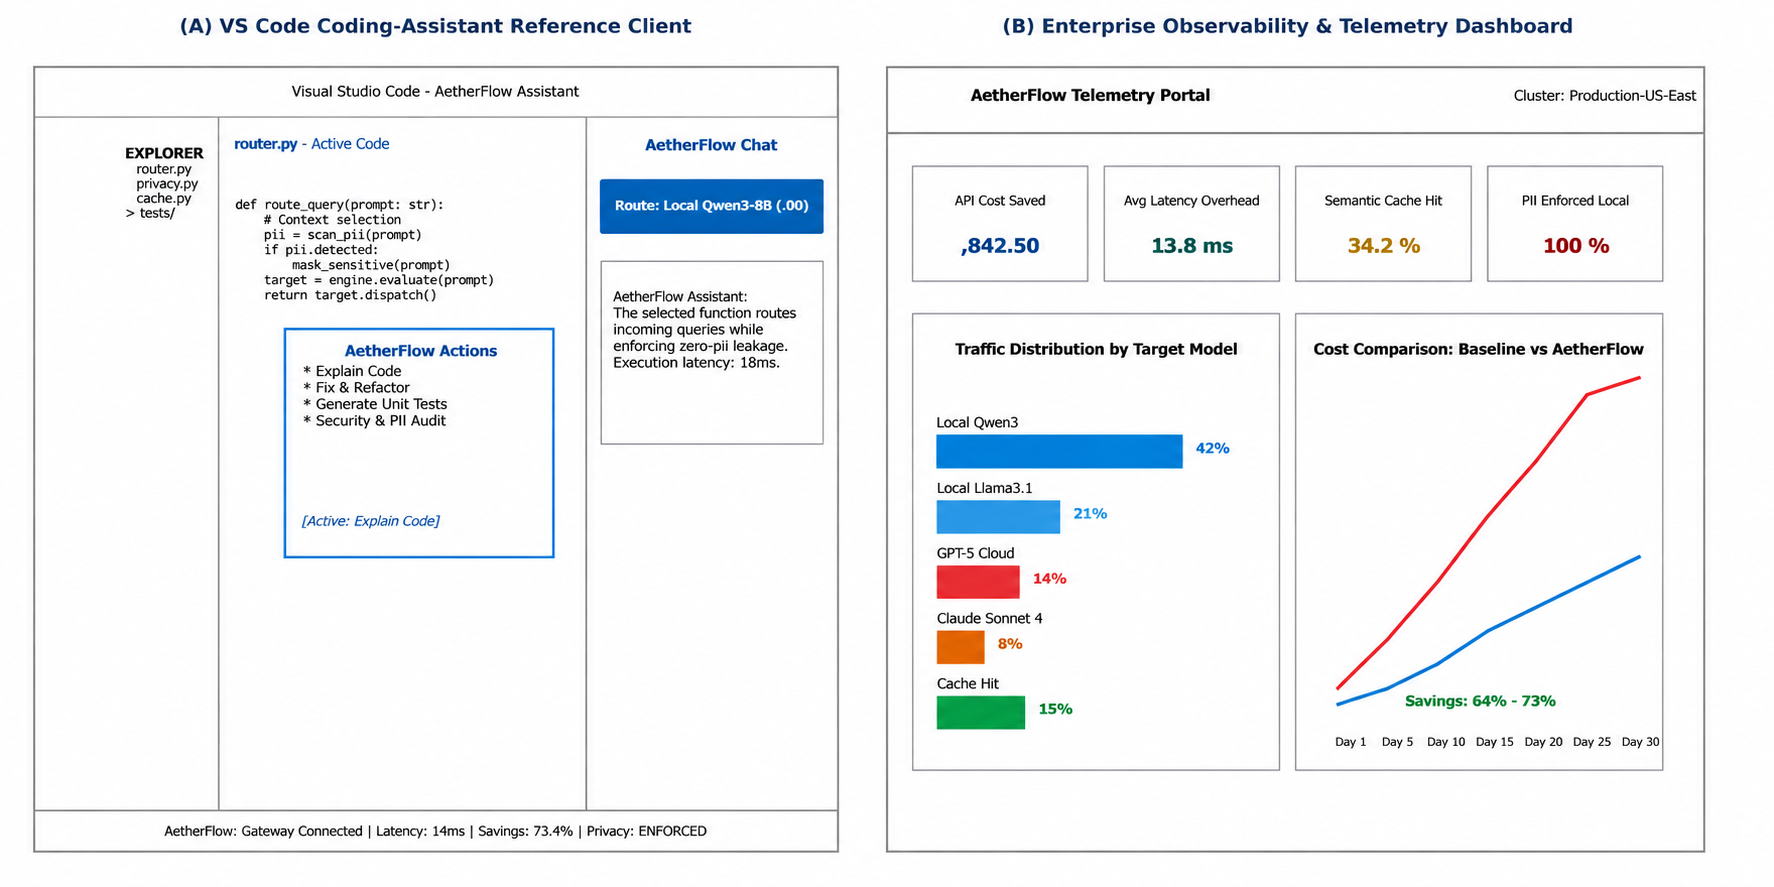
\includegraphics[height=0.43\textheight,trim=0bp 0bp 914bp 0bp,clip]{Figures/gui_mockups_white.png}
\par\vspace{0.5em}
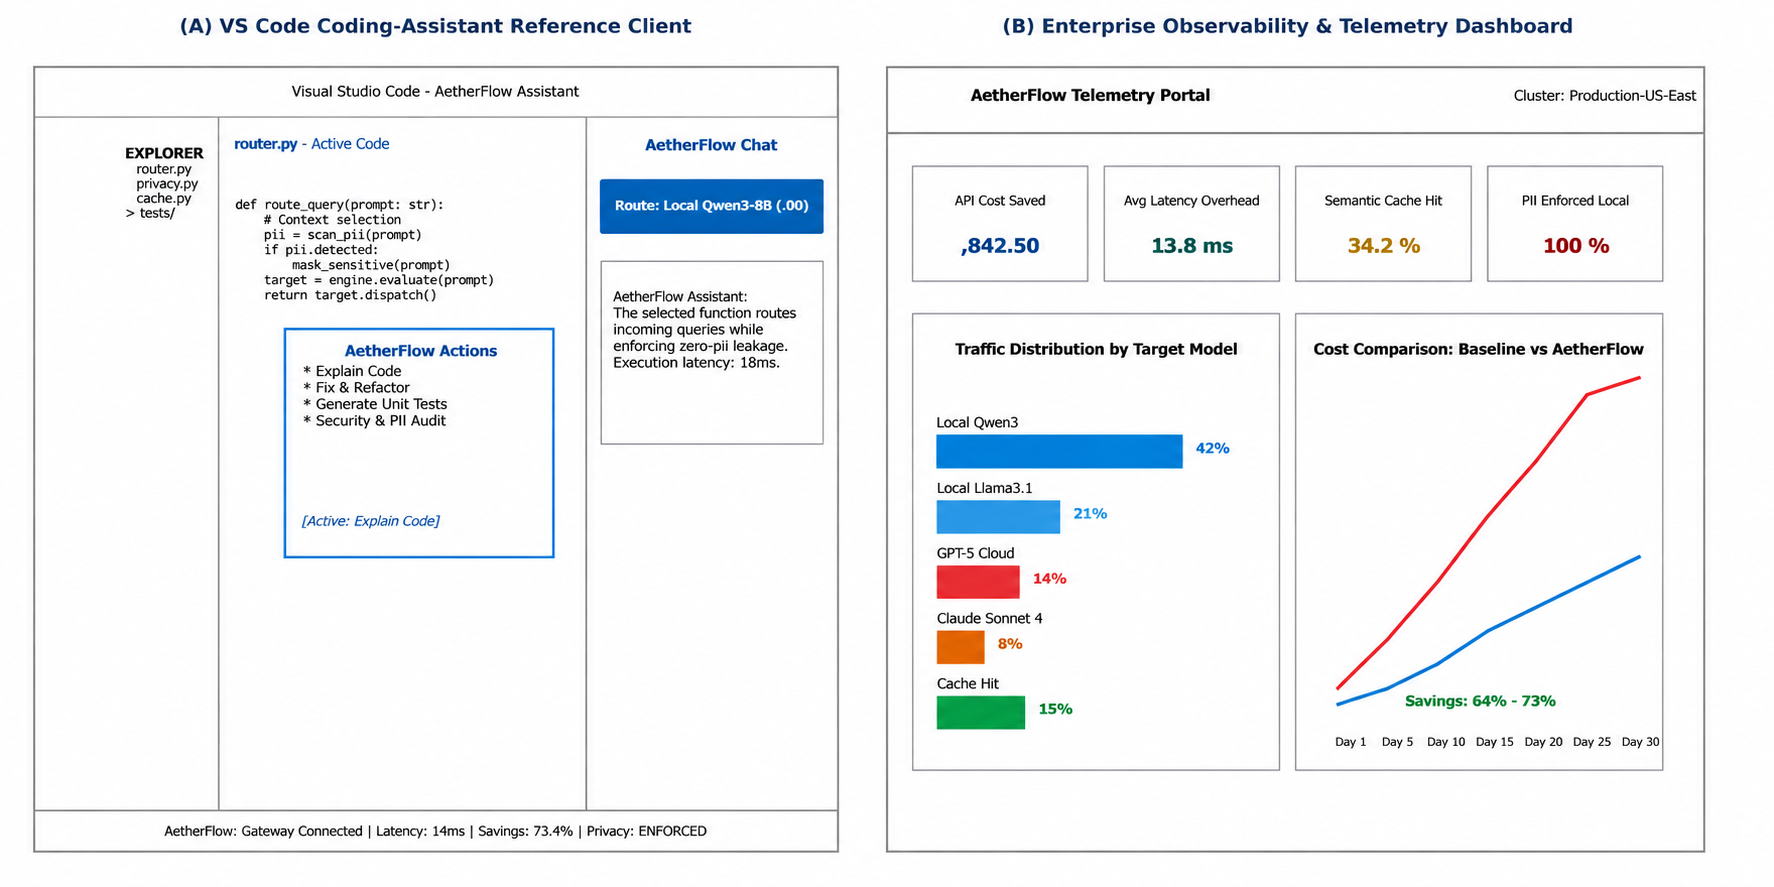
\includegraphics[height=0.43\textheight,trim=870bp 0bp 0bp 0bp,clip]{Figures/gui_mockups_white.png}
\caption{AetherFlow GUI mockups with high detail: (A) Visual Studio Code developer add-on and (B) Enterprise telemetry and admin screen.}
\label{fig:gui_mockups}
\end{figure}

\subsection{Developer Client Interface (VS Code Extension)}
The VS Code add-on shown in Figure~\ref{fig:gui_mockups}A is intended to
support common code-assistance tasks:
\begin{enumerate}
    \item \textbf{Context menu actions:} The developer selects code, opens the
    context menu, and chooses one of the available actions:
    \begin{itemize}
        \item \textit{``AetherFlow: Explain Code''}
        \item \textit{``AetherFlow: Refactor Code''}
        \item \textit{``AetherFlow: Generate Tests''}
    \end{itemize}
    These actions support Use Case UC-01.
    \item \textbf{Sidebar panel:} The client is intended to display the
    response in a markdown panel, with formatted code blocks and, where
    available, a short explanation of the change.
    \item \textbf{Split view:} For a refactoring request, the proposed
    interface displays the original code beside the suggested replacement.
    An ``Apply to Editor'' action may then be used to insert the suggestion
    after the developer has reviewed it.
    \item \textbf{Status bar badge:} After a request, the status bar may show
    the execution source and diagnostic information, for example
    \texttt{"AetherFlow: Local (Qwen3-8B) | Saved \$0.04 | 142ms"}. The
    interface should identify simulated or unavailable values. A privacy
    result and latency breakdown may be shown when those measurements are
    available. The example badge is illustrative and is not a measurement.
\end{enumerate}

\subsection{Enterprise Administrator Interface (Telemetry Dashboard)}
The dashboard in Figure~\ref{fig:gui_mockups}B is a proposed interface for
monitoring and administering the gateway:
\begin{enumerate}
    \item \textbf{Group status panels:} Display the health, memory use, and
    response time of PostgreSQL, Qdrant, local model services, and configured
    external providers.
    \item \textbf{Throughput gauges:} Display request rate, active streaming
    sessions, and measured gateway overhead.
    \item \textbf{Routing chart:} Show the proportion of responses served by
    the cache, local models, and external providers.
    \item \textbf{Policy weight sliders:} Allow an authorized administrator to
    edit the quality ($w_q$), cost ($w_c$), and latency ($w_l$) weights for
    Use Case UC-04, subject to policy validation.
    \item \textbf{Audit log:} Show permitted metadata such as the event time,
    client reference, classification outcome, execution source, and runtime.
    Raw prompts, credentials, temporary mappings, and restored sensitive values
    shall not be displayed.
\end{enumerate}

\subsection{Low-Fidelity Prototyping Wireframes}
The wireframes in Figure~\ref{fig:lowfi_wireframes} are early design
proposals. Part (a) shows the developer extension, and part (b) shows the
telemetry and policy dashboard. These wireframes describe the intended layout;
they do not demonstrate that the illustrated backend functions are already
available.

\begin{figure}[!htbp]
\centering
\begin{minipage}{0.48\textwidth}
    \centering
    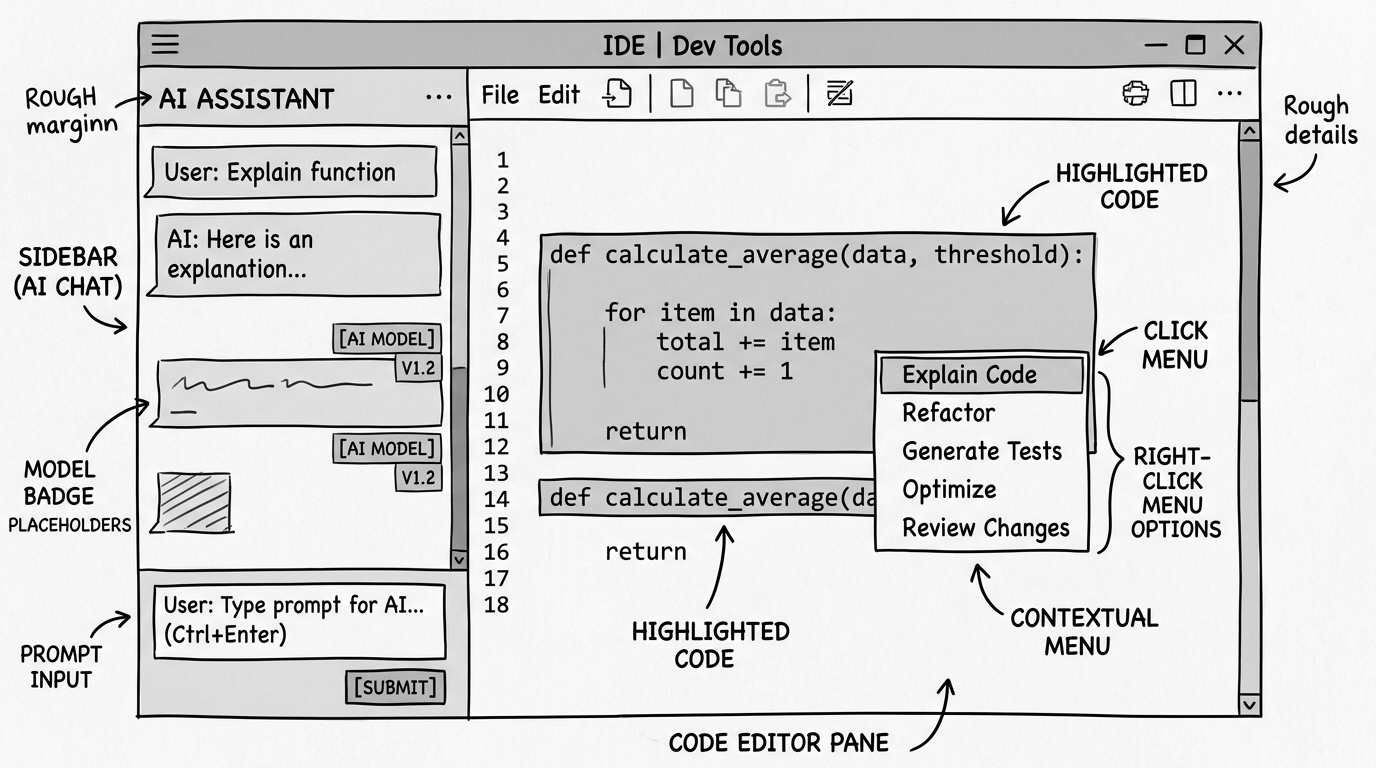
\includegraphics[width=\linewidth]{Figures/low_fi_ide.jpg}
    \caption*{(a) Developer Extension Wireframe}
\end{minipage}\hfill
\begin{minipage}{0.48\textwidth}
    \centering
    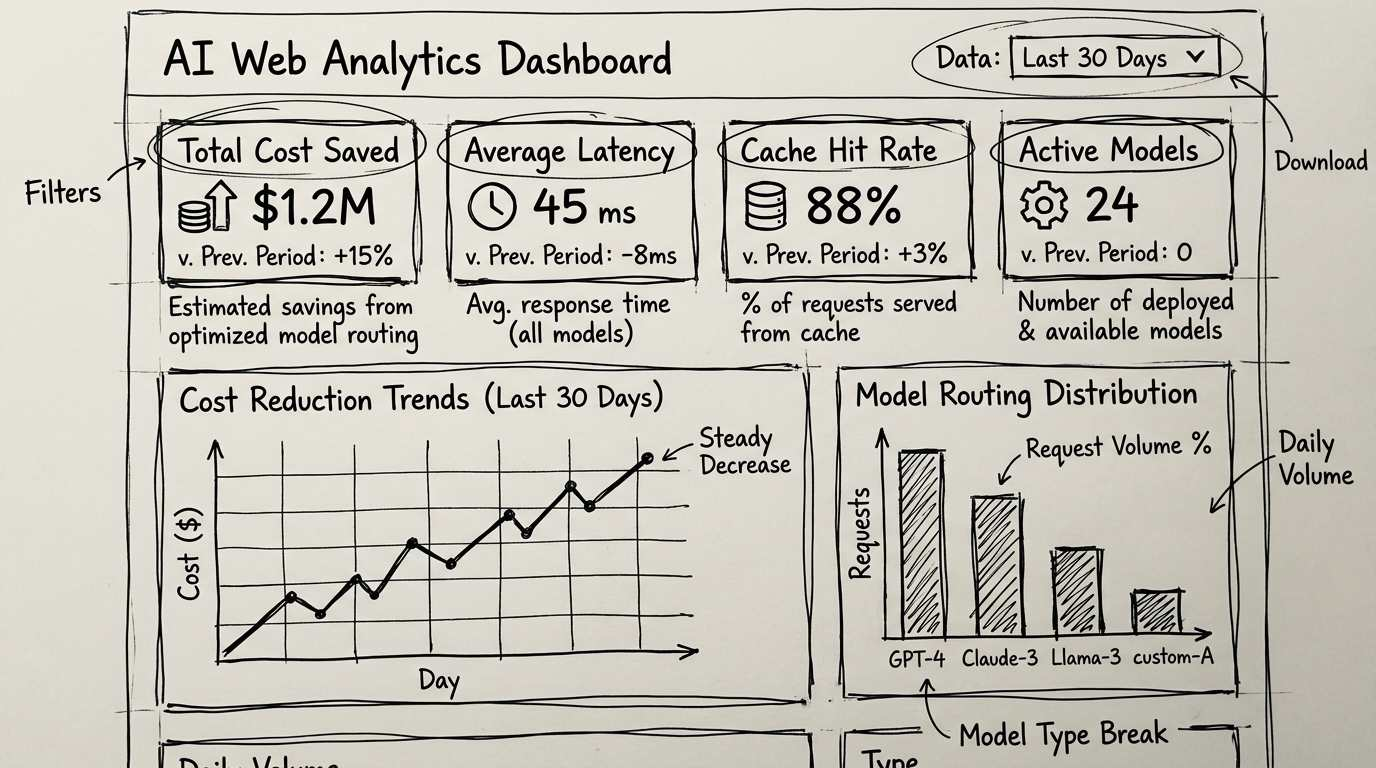
\includegraphics[width=\linewidth]{Figures/low_fi_dashboard.jpg}
    \caption*{(b) Telemetry Dashboard Wireframe}
\end{minipage}
\caption{AetherFlow low fidelity prototype layouts: (a) Visual Studio Code developer client extension and (b) Enterprise telemetry and policy dashboard.}
\label{fig:lowfi_wireframes}
\end{figure}

\subsection{Implemented VS Code Extension Prototype}
The available AetherFlow Assistant client prototype is shown in
Figure~\ref{fig:vscode_prototype}. Inspection of its TypeScript source found
commands for Explain, Fix, Refactor, and Generate Tests in the webview chat
panel. The prototype also has a default mock mode and can send a JSON request
to the \texttt{/chat} endpoint. When a response does not contain metadata, the
client supplies illustrative default values. These defaults are interface
placeholders and must not be treated as gateway measurements.

The inspected code does not yet provide the proposed SSE integration,
production authentication, privacy analyzer, operational vault, trained
router, or database services. The client will therefore require integration
changes before it can use the planned \texttt{/v1/chat/completions} contract.
Figure~\ref{fig:vscode_prototype} documents interface work only. Existing mock
provider names and values are prototype artifacts; the proposed deployment
pool is specified in Chapters~\ref{ch:methodology} and~\ref{ch:design}.



\section{Database Design}
\label{sec:database-design}
The proposed persistence design separates relational records in PostgreSQL
from vector points in Qdrant. PostgreSQL will be authoritative for clients,
policy versions, model configurations, request state, cache state, and audit
metadata. Qdrant will support filtered approximate retrieval for embeddings
belonging to approved plain requests. No migration repository or deployed
database was available for verification at the time of writing. This section
therefore describes the schema planned for implementation, not an existing
production database.

A PostgreSQL cache record and its Qdrant point will use the same UUID. The
application will maintain this association because a foreign key cannot span
the two databases. Qdrant retrieval alone will not authorize a response.
Before returning cached text, the gateway must recheck ownership, policy and
context compatibility, readiness, and expiry using PostgreSQL. Temporary
placeholder mappings will remain in a separate encrypted, volatile vault;
neither the relational records nor the vector payloads will store those
mappings.

\begin{figure}[H]
\centering
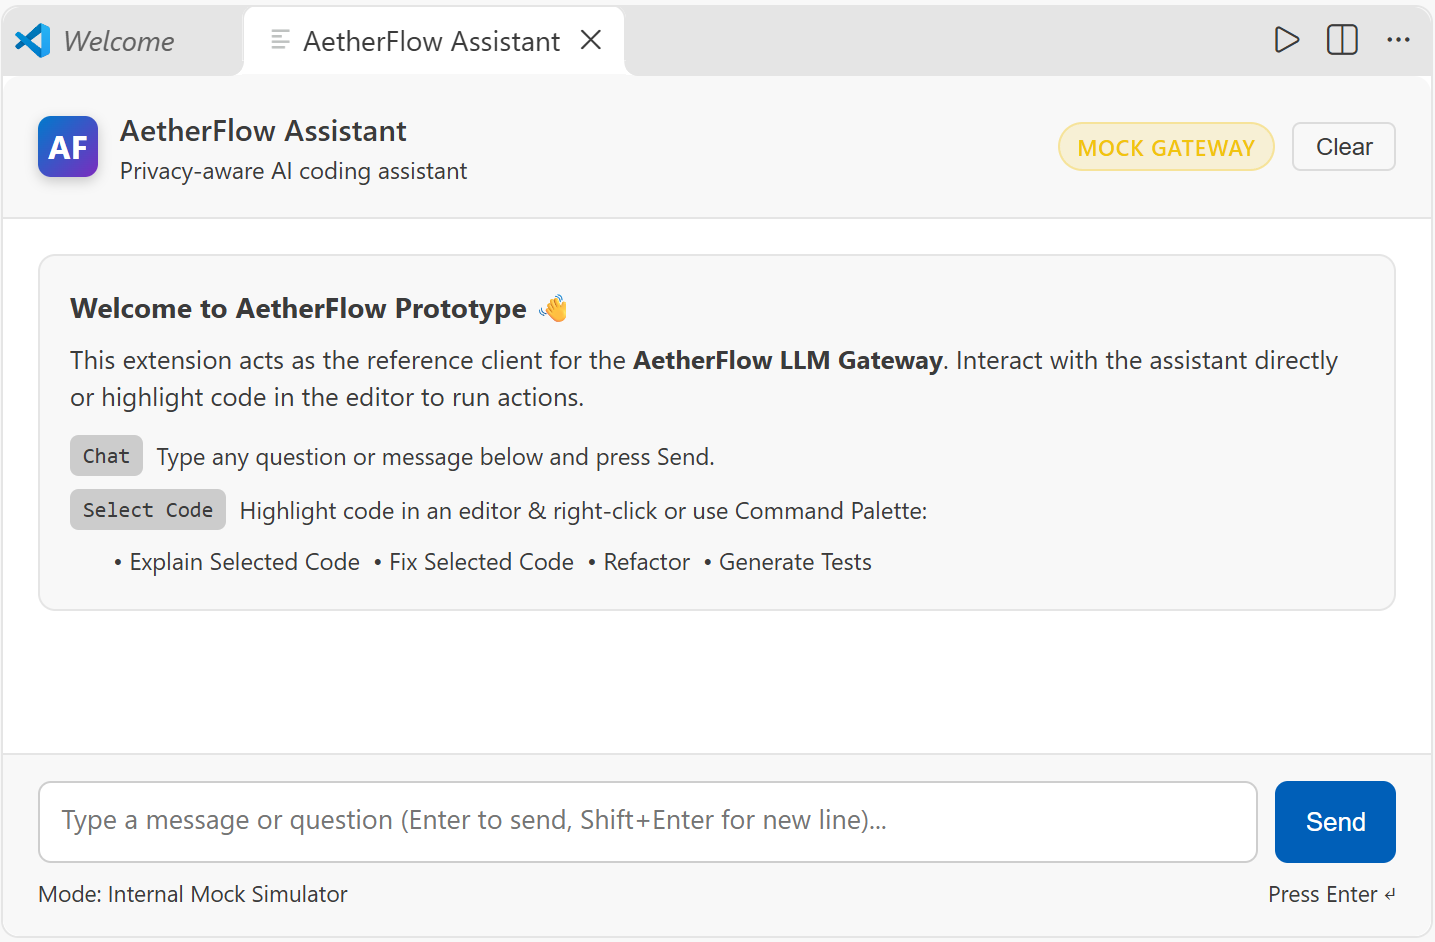
\includegraphics[width=\textwidth,height=0.52\textheight]{Figures/vscode_assistant_prototype.png}
\caption{Prototype for the AetherFlow Assistant VS Code extension: Chat interface with code-aware actions and gateway connectivity indicator.}
\label{fig:vscode_prototype}
\end{figure}

\subsection{ER Diagram}
\label{subsec:er-diagram}
AetherFlow's relational data tier is represented using traditional
\textbf{Chen notation}, as shown in Figure~\ref{fig:er_diagram}. Rectangles
represent entities, ellipses represent conceptual attributes, and underlined
attributes identify primary keys. Diamonds represent relationships, with
cardinality ratios such as $1:1$ and $1:N$. Foreign keys are omitted from the
conceptual diagram to keep it readable; their proposed relational definitions
are documented in the data dictionary in Section~\ref{subsec:data-dictionary}.

\begin{figure}[p]
\centering
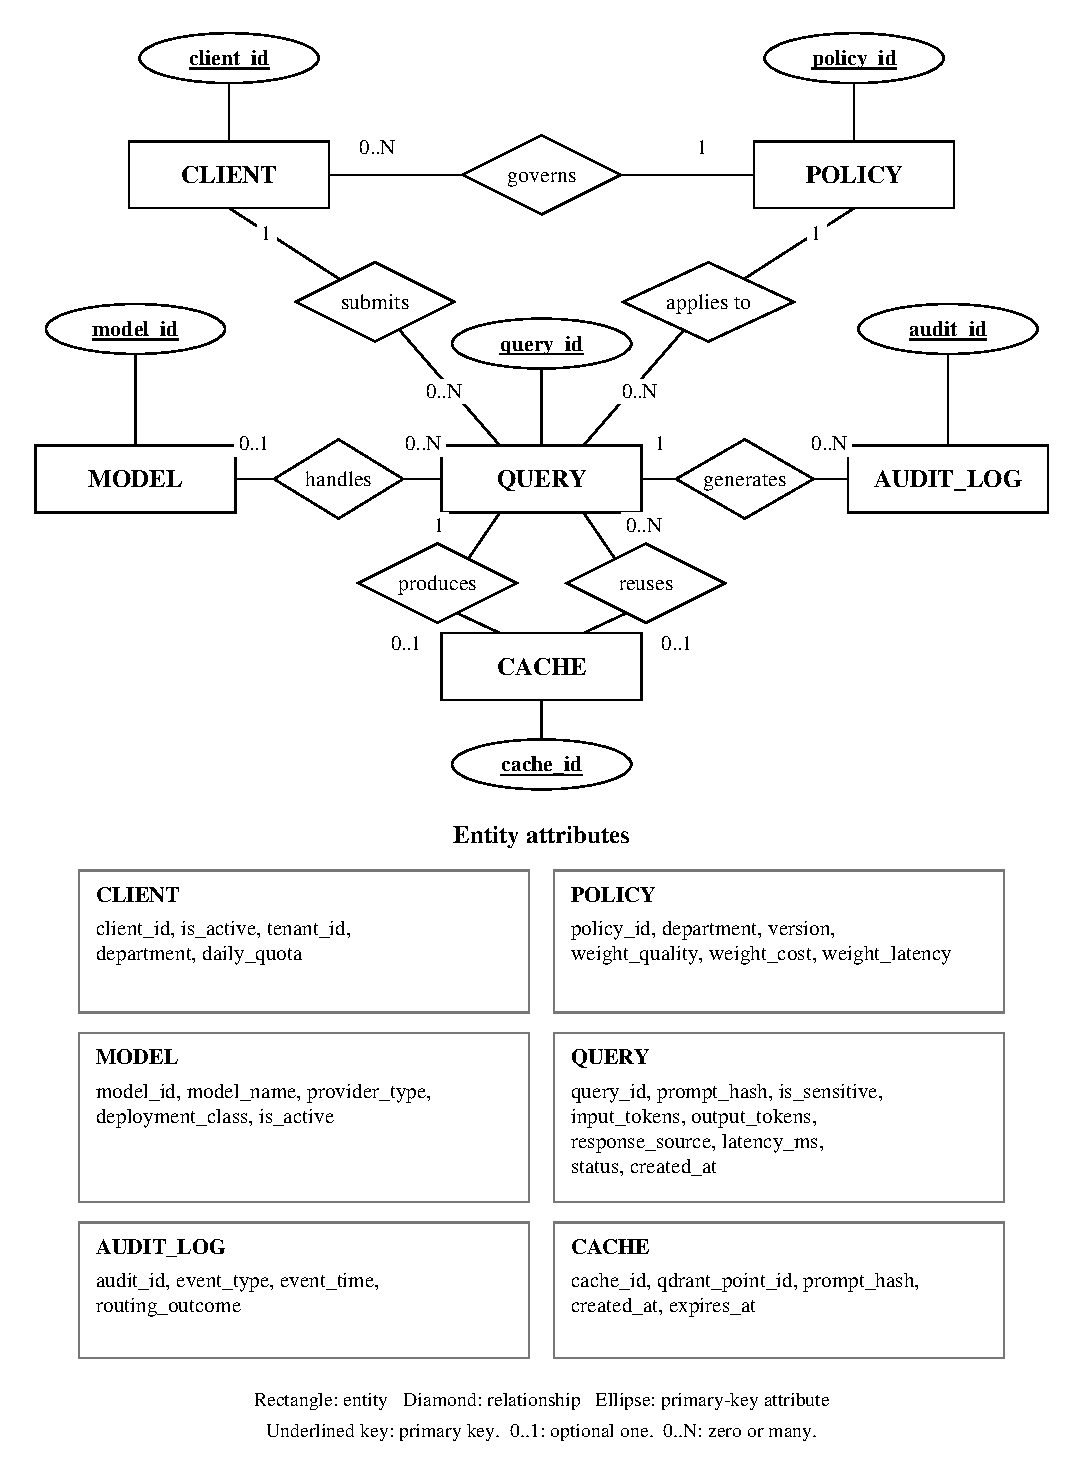
\includegraphics[width=\textwidth,height=0.92\textheight,keepaspectratio]{Figures/er_postgresql.pdf}
\caption{Proposed Chen-notation Entity-Relationship (ER) diagram for AetherFlow.}
\label{fig:er_diagram}
\end{figure}

The proposed conceptual model consists of six operational entities and seven
relationships:

\begin{enumerate}
    \item \textbf{POLICY governs CLIENT ($1 : 0..N$):} A policy may govern zero or more authenticated clients within a tenant. Each client is assigned one active policy version.
    \item \textbf{CLIENT submits QUERY ($1 : 0..N$):} A client may submit zero or more queries during its lifetime. Each query belongs to one authenticated client.
    \item \textbf{POLICY applies to QUERY ($1 : 0..N$):} A policy version may apply to zero or more queries. Each query records the exact policy version used for its decision so that the decision remains auditable.
    \item \textbf{MODEL handles QUERY ($0..1 : 0..N$):} A registered local or cloud model may handle zero or more queries. A query may reference zero or one final model because cache hits and requests rejected before routing do not have a selected model. A bounded attempt record can retain information about an unsuccessful attempt.
    \item \textbf{QUERY returns CACHE ($1 : 0..1$):} A query that completes direct inference may create zero or one approved cache entry. Each cache entry records the query that produced it.
    \item \textbf{QUERY reuses CACHE ($0..1 : 0..N$):} An incoming query may reuse zero or one cache entry. One cache entry may be reused by many later queries when all verification checks succeed. Cache creation and cache reuse are represented separately because they have different purposes.
    \item \textbf{QUERY generates AUDIT\_LOG ($0..1 : 0..N$):} A query may generate zero or more append-only audit events. These events record permitted metadata about screening, routing, and execution. Request events reference a query, while administrative events may have a null query reference. Tenant and actor information remains required for both types of event.
\end{enumerate}

\subsection{Data Dictionary}
\label{subsec:data-dictionary}
Table~\ref{tab:data_dict_table} describes the six proposed PostgreSQL
entities. It lists the column names, PostgreSQL-compatible data types,
integrity constraints, and intended purpose of each field. The constraints
include primary keys, foreign keys, uniqueness, required values, checks, and
defaults. This dictionary documents the planned relational design; it is not a
record of an already deployed schema.


\begingroup
\footnotesize
\setlength{\tabcolsep}{3.5pt}
\renewcommand{\arraystretch}{1.08}
\begin{longtable}{|P{3.5cm}|P{2.3cm}|P{2.5cm}|P{6.3cm}|}
\caption{Proposed PostgreSQL relational data dictionary}\label{tab:data_dict_table}\\
\hline
\textbf{Entity / Column} & \textbf{Data Type} & \textbf{Constraints} & \textbf{Description} \\ \hline
\endfirsthead
\hline
\textbf{Entity / Column} & \textbf{Data Type} & \textbf{Constraints} & \textbf{Description (continued)} \\ \hline
\endhead
\hline
\endfoot
\multicolumn{4}{|c|}{\textbf{POLICY}} \\* \hline
\texttt{policy\_id} & UUID & PK, NOT NULL & Immutable identifier for one version of a routing policy. \\ \hline
\texttt{tenant\_id} & UUID & NOT NULL & Organization or tenant to which the policy belongs. \\ \hline
\texttt{department} & VARCHAR(64) & NOT NULL & Department or organizational unit governed by the policy. \\ \hline
\texttt{version} & INTEGER & NOT NULL, CHECK ($>0$) & Positive version number, unique within the tenant and department. \\ \hline
\texttt{weight\_quality} & NUMERIC(4,3) & NOT NULL, CHECK ($0 \le w_q \le 1$) & Weight assigned to the quality term in the utility function. \\ \hline
\texttt{weight\_cost} & NUMERIC(4,3) & NOT NULL, CHECK ($0 \le w_c \le 1$) & Weight assigned to the cost term in the utility function. \\ \hline
\texttt{weight\_latency} & NUMERIC(4,3) & NOT NULL, CHECK ($0 \le w_l \le 1$) & Weight assigned to the latency term; $w_q+w_c+w_l=1$. Privacy remains a hard constraint rather than a utility weight. \\ \hline
\texttt{privacy\_rules} & JSONB & NOT NULL & Policy rules for local residency, approved masking, and restricted entity classes. \\ \hline
\texttt{norm\_bounds} & JSONB & NOT NULL & Reference minimum and maximum values used to normalize cost and latency. \\ \hline
\texttt{daily\_token\_cap} & BIGINT & NOT NULL, CHECK ($\ge 0$) & Maximum cumulative tokens allowed for the department in one day. \\ \hline
\texttt{monthly\_usd\_cap} & NUMERIC(14,6) & NOT NULL, CHECK ($\ge 0$) & Maximum monthly cloud-provider spending for the department, in USD. \\ \hline
\texttt{created\_at} & TIMESTAMPTZ & NOT NULL, DEFAULT now() & UTC time at which this policy version was registered. \\ \hline
\multicolumn{4}{|c|}{\textbf{CLIENT}} \\* \hline
\texttt{client\_id} & UUID & PK, NOT NULL & Identifier assigned to an authenticated gateway client. \\ \hline
\texttt{tenant\_id} & UUID & NOT NULL & Tenant used to isolate this client from other organizations. \\ \hline
\texttt{department} & VARCHAR(64) & NOT NULL & Organizational unit associated with the client. \\ \hline
\texttt{policy\_id} & UUID & FK: POLICY, NOT NULL & Active policy version assigned to the client. \\ \hline
\texttt{api\_key\_hash} & VARCHAR(64) & UNIQUE, NOT NULL & SHA-256 digest of the client credential; the plaintext credential is not stored. \\ \hline
\texttt{daily\_quota} & BIGINT & NOT NULL, CHECK ($\ge 0$) & Maximum number of tokens the client may use per day. \\ \hline
\texttt{is\_active} & BOOLEAN & NOT NULL, DEFAULT true & Flag used to enable or suspend the client account. \\ \hline
\texttt{created\_at} & TIMESTAMPTZ & NOT NULL, DEFAULT now() & UTC time at which the client account was created. \\ \hline
\multicolumn{4}{|c|}{\textbf{MODEL}} \\* \hline
\texttt{model\_id} & VARCHAR(64) & PK, NOT NULL & Stable identifier for a registered backend, such as \texttt{vllm-qwen3-8b}. \\ \hline
\texttt{model\_name} & VARCHAR(64) & NOT NULL & Model revision and deployment configuration; a changed revision receives a new identifier. \\ \hline
\texttt{provider\_type} & VARCHAR(32) & NOT NULL & Adapter family, such as \texttt{vLLM}, \texttt{Ollama}, \texttt{OpenAI}, or \texttt{Gemini}. \\ \hline
\texttt{deployment\_class} & VARCHAR(8) & NOT NULL, CHECK in ('local', 'cloud') & Indicates whether the backend is local or external for residency filtering. \\ \hline
\texttt{endpoint} & TEXT & NOT NULL & Network endpoint for the model service; credentials must not be embedded in the URI. \\ \hline
\texttt{credential\_ref} & TEXT & NULL & Reference to protected credentials for an external provider. \\ \hline
\texttt{cost\_in\_per\_1k} & NUMERIC(14,6) & NOT NULL, CHECK ($\ge 0$) & Cost in USD per 1,000 input tokens; local models may use zero. \\ \hline
\texttt{cost\_out\_per\_1k} & NUMERIC(14,6) & NOT NULL, CHECK ($\ge 0$) & Cost in USD per 1,000 generated tokens; local models may use zero. \\ \hline
\texttt{rolling\_latency} & DOUBLE PRECISION & NULL, CHECK ($>0$) & Recent estimated latency in seconds; NULL when no valid measurement exists. \\ \hline
\texttt{is\_active} & BOOLEAN & NOT NULL, DEFAULT true & Flag used to include or exclude the backend from candidate selection. \\ \hline
\multicolumn{4}{|c|}{\textbf{QUERY}} \\* \hline
\texttt{query\_id} & UUID & PK, NOT NULL & Identifier generated for each incoming gateway request. \\ \hline
\texttt{client\_id} & UUID & FK: CLIENT, NOT NULL & Authenticated client that submitted the request. \\ \hline
\texttt{policy\_id} & UUID & FK: POLICY, NOT NULL & Policy version captured when the request was evaluated. \\ \hline
\texttt{model\_id} & VARCHAR(64) & FK: MODEL, NULL & Final selected backend; NULL for cache hits and requests rejected before model selection. Earlier attempts are recorded separately. \\ \hline
\texttt{cache\_id} & UUID & FK: CACHE, NULL & Cache entry used for a verified hit; NULL when the response came from model inference. \\ \hline
\texttt{prompt\_hash} & VARCHAR(64) & NULL & Keyed HMAC-SHA-256 fingerprint of an approved plain prompt; NULL for masked or restricted input. \\ \hline
\texttt{input\_tokens} & BIGINT & NULL, CHECK ($\ge 0$) & Reconciled input-token total across the request's attempts. \\ \hline
\texttt{output\_tokens} & BIGINT & NULL, CHECK ($\ge 0$) & Reconciled generated-token total; zero for a cache-only response. \\ \hline
\texttt{cost\_usd} & NUMERIC(14,6) & NULL, CHECK ($\ge 0$) & Reconciled provider cost; NULL while usage remains unresolved. \\ \hline
\texttt{privacy\_class} & VARCHAR(16) & NOT NULL & Request classification: \texttt{plain}, \texttt{maskable}, \texttt{restricted}, or \texttt{rejected}. \\ \hline
\texttt{response\_source} & VARCHAR(16) & NOT NULL & Provenance: \texttt{none}, \texttt{cache\_hit}, \texttt{local\_model}, or \texttt{cloud\_api}. \\ \hline
\texttt{status} & VARCHAR(16) & NOT NULL & Lifecycle state: received, running, completed, failed, rejected, or cancelled. \\ \hline
\texttt{latency\_ms} & DOUBLE PRECISION & NULL, CHECK ($\ge 0$) & End-to-end response time measured by the gateway or proxy. \\ \hline
\texttt{created\_at} & TIMESTAMPTZ & NOT NULL, DEFAULT now() & UTC time at which the request was received. \\ \hline
\texttt{reserved\_tokens} & BIGINT & NOT NULL, DEFAULT 0, CHECK ($\ge0$) & Outstanding conservative token reservations for the request. \\ \hline
\texttt{reserved\_usd} & NUMERIC(14,6) & NOT NULL, DEFAULT 0, CHECK ($\ge0$) & Outstanding bounded provider charges, including unresolved attempts. \\ \hline
\texttt{usage\_state} & VARCHAR(16) & NOT NULL & Usage status: none, reserved, reconciled, or unresolved. This separates unknown usage from zero cost. \\ \hline
\texttt{attempts} & JSONB & NOT NULL, DEFAULT [] & Up to two validated attempt summaries containing identifiers, reservations, usage, status, and timing; no prompts or secrets. \\ \hline
\texttt{decision\_meta} & JSONB & NOT NULL, DEFAULT \{\} & Predictor version, policy-bound estimates, normalization bounds, utility, exclusions, and stage timings; no raw request text. \\ \hline
\multicolumn{4}{|c|}{\textbf{CACHE}} \\* \hline
\texttt{cache\_id} & UUID & PK, NOT NULL & Identifier shared by the PostgreSQL cache record and its Qdrant point. \\ \hline
\texttt{source\_query\_id} & UUID & FK: QUERY, UNIQUE, NOT NULL & Direct-inference query that produced the approved cached response. \\ \hline
\texttt{qdrant\_point\_id} & UUID & UNIQUE, NOT NULL & Qdrant point identifier, normally equal to \texttt{cache\_id}. \\ \hline
\texttt{collection\_name} & VARCHAR(128) & NOT NULL & Versioned Qdrant collection containing the vector point. \\ \hline
\texttt{prompt\_hash} & VARCHAR(64) & NOT NULL & Keyed fingerprint of the approved plain prompt used for exact verification. \\ \hline
\texttt{context\_hash} & VARCHAR(64) & NOT NULL & Fingerprint of the system/history context, project revision, model revision, generation settings, and response-schema version. \\ \hline
\texttt{response\_text} & TEXT & NULL & Approved response text; retained only while the entry is ready and within its retention period. \\ \hline
\texttt{state} & VARCHAR(16) & NOT NULL & Cache lifecycle state: \texttt{pending}, \texttt{ready}, \texttt{expired}, or \texttt{revoked}. \\ \hline
\texttt{hit\_count} & BIGINT & NOT NULL, CHECK ($\ge 0$), DEFAULT 0 & Number of successful responses served from this entry. \\ \hline
\texttt{created\_at} & TIMESTAMPTZ & NOT NULL, DEFAULT now() & UTC time at which the cache record was committed. \\ \hline
\texttt{expires\_at} & TIMESTAMPTZ & NOT NULL, CHECK ($> \text{\texttt{created\_at}}$) & UTC time after which the entry must not be served. \\ \hline
\multicolumn{4}{|c|}{\textbf{AUDIT\_LOG}} \\* \hline
\texttt{audit\_id} & UUID & PK, NOT NULL & Identifier for one audit event. \\ \hline
\texttt{query\_id} & UUID & FK: QUERY, NULL & Related request identifier; NULL for an administrative event. \\ \hline
\texttt{tenant\_id} & UUID & NOT NULL & Server-derived tenant associated with the request or administrator. \\ \hline
\texttt{actor\_ref} & TEXT & NOT NULL & Reference to the authenticated client or administrator, not an API credential. \\ \hline
\texttt{event\_type} & VARCHAR(32) & NOT NULL & Category such as screening, vault, cache, routing, execution, billing, or policy change. \\ \hline
\texttt{detected\_\allowbreak entity\_\allowbreak types} & TEXT[] & NULL & Sanitized entity categories, such as \texttt{['API\_KEY']}; original values are excluded. \\ \hline
\texttt{masking\_applied} & BOOLEAN & NOT NULL, DEFAULT false & Indicates whether approved values were replaced with vault placeholders. \\ \hline
\texttt{routing\_outcome} & VARCHAR(32) & NOT NULL & Outcome such as pending, cache, local, cloud, rejected, failed, or administrative. \\ \hline
\texttt{details} & JSONB & NOT NULL & Additional approved metadata, such as token counts or latency stages; no plaintext secrets. \\ \hline
\texttt{created\_at} & TIMESTAMPTZ & NOT NULL, DEFAULT now() & UTC time at which the append-only audit event was created. \\ \hline
\end{longtable}
\endgroup

\noindent\textbf{Relational integrity and quota accounting.}
Each policy version is immutable and is unique for the combination of tenant,
department, and version number. A client is assigned to one tenant,
department, and active policy. When a new policy is published, new requests
use the new policy reference, while existing requests retain the policy
version captured at admission. The baseline design does not move a client
between departments; such a change would require an explicit administrative
operation.

A completed request must have either a selected \texttt{model\_id} or a
reused \texttt{cache\_id}, but not both. Requests that fail or are rejected
before completion may have neither value. The uniqueness of
\texttt{CACHE.source\_query\_id} ensures that one direct-inference query
creates at most one source cache entry. Conditions involving several rows
cannot be enforced reliably with an ordinary row-level CHECK constraint, so
the implementation will use transactions and, where necessary, triggers or
application validation. PostgreSQL state remains authoritative when checking
whether a cache entry is ready, owned by the correct scope, and unexpired.
The tenant recorded in a request audit event must match the request and client
tenant. Administrative events use an authenticated actor and a null
\texttt{query\_id}.

For the baseline design, at most two attempt summaries are stored in
\texttt{QUERY.attempts} rather than creating a separate attempt table. The
application must validate the structure and model references in each summary;
the identifiers inside the JSON are not SQL foreign keys. A future migration
may normalize this data if more detailed attempt history is required.
Reservation fields summarize outstanding ledger activity; they are not
independent usage counters. Token and spending admission will use a
consistent transaction-locking protocol for the relevant tenant and
department. Usage is assigned to the UTC day and month in which admission
occurred, independently of a provider's invoice period.

The admission transaction will reserve the bounded usage before network
dispatch. Reconciliation will replace the reservation with measured usage
when provider information becomes available, while unresolved reservations
will be retained. A worker failure must not remove a reservation merely
because the client disconnected. Proposed indexes cover request
client/time, policy/time, cache state/expiry, source query, and audit
tenant/time. A separate production-scale aggregation ledger is not assumed
for the baseline implementation.

\noindent\textbf{Encrypted storage and retention of map data.}
The proposed vault is a separate, volatile store used only for the duration of
a request. Its envelope will contain an opaque mapping identifier, the tenant,
client, and query identifiers, the policy version, an expiry time, the
algorithm identifier, a nonce, an authentication tag, and a protected
key-wrapping reference. The mapping between a placeholder and its original
value will remain encrypted. Neither the mapping nor plaintext data keys will
be stored in PostgreSQL, Qdrant, or routine audit metadata. The associated
metadata used for authentication will be included as authenticated associated
data. If the mapping or its key handle is destroyed, restoration cannot
continue. The proposed maximum lifetime is five minutes, or the shorter
request deadline.

Approved cache responses have an initial proposed TTL of 24 hours. When an
entry expires or is revoked, the response text will be cleared and its Qdrant
point will be removed. A minimal PostgreSQL tombstone may retain the historical
\texttt{QUERY.cache\_id} for audit purposes. Related metadata may initially be
retained for 30 days, subject to organizational policy. Purging must respect
foreign-key dependencies and follow a documented transaction order. Application
roles will not be allowed to update or delete audit events during the retention
period; an authorized retention job will perform expiry processing. Append-only
permissions alone do not provide cryptographic tamper evidence. Signed audit
exports could be added later, but would require a separate key-management and
audit process.

\noindent\textbf{Qdrant collection schema (non-relational).}
The proposed versioned collection \texttt{aetherflow\_cache\_v1} stores
384-dimensional embeddings and uses cosine distance
\cite{ref:MiniLM,ref:Qdrant}. Table~\ref{tab:qdrant_dict_table} describes
the point fields and payload keys; it is not a relational schema and does not
define foreign keys. Payload indexes support filtering by client, tenant,
policy, and context, while a range filter supports expiry checks. A new
collection will be required if the embedding checkpoint, tokenizer behaviour,
or vector dimension changes. Existing vectors must not be compared with
incompatible vectors without re-embedding and revalidation.

\begin{table}[H]
\centering
\small
\setlength{\tabcolsep}{4pt}
\renewcommand{\arraystretch}{1.12}
\begin{tabular}{|P{3.8cm}|P{2.4cm}|P{8.0cm}|}
\hline
\textbf{Field / Payload Key} & \textbf{Data Type} & \textbf{Purpose and Retrieval Constraints} \\ \hline
\texttt{id} & UUID & Point identifier matching the PostgreSQL \texttt{CACHE.cache\_id}. \\ \hline
\texttt{vector} & Dense Float[384] & Prompt embedding generated by \texttt{all-MiniLM-L6-v2} for cosine retrieval. \\ \hline
\texttt{payload.prompt} & String & Approved plain prompt used during candidate verification. \\ \hline
\texttt{payload.tenant\_id} & UUID (String) & Server-derived tenant scope, checked again in PostgreSQL. \\ \hline
\texttt{payload.client\_id} & UUID (String) & Authenticated source client used for initial per-client filtering. \\ \hline
\texttt{payload.policy\_id} & UUID (String) & Policy version used to isolate cache entries. \\ \hline
\texttt{payload.prompt\_hash} & String & Keyed prompt fingerprint; a match does not bypass the remaining checks. \\ \hline
\texttt{payload.context\_hash} & String & Fingerprint of the context, model revision, and response-schema revision. \\ \hline
\texttt{payload.expires\_at} & Integer (Unix) & UTC expiry time used by the range filter before authoritative verification. \\ \hline
\end{tabular}
\caption{Proposed Qdrant vector collection point and payload schema.}
\label{tab:qdrant_dict_table}
\end{table}

Cache publication is a recoverable multi-step workflow rather than a
distributed atomic transaction. The application first records a pending
PostgreSQL entry, then performs an idempotent Qdrant upsert, and marks the
entry ready only after the vector write is confirmed. Pending entries are
never served. A reconciliation job can repair or expire incomplete writes. If
the process crashes after the Qdrant upsert, the remaining point is
unservable until PostgreSQL confirms the corresponding ready record.

During lookup, the application filters candidates by scope and expiry in
Qdrant, checks the candidate data, and then rechecks PostgreSQL ownership,
state, context compatibility, and expiry before delivery. PostgreSQL response
text is authoritative. A stale vector, missing row, incompatible context, or
unavailable store causes a cache miss. Updating PostgreSQL before deleting a
revoked vector ensures that delayed vector deletion cannot authorize reuse.
Masked-request mappings, raw credentials, and restored sensitive values are
not stored in either cache system.

\section{Risk Analysis}
\label{sec:risk-analysis}
The ratings in Table~\ref{tab:risk_analysis} are qualitative planning
judgements, not measured probabilities. They consider both the possible
frequency of a problem and the consequence if it occurs. The mitigations
describe the proposed controls and still require implementation and testing.
The final column also records important limitations that the controls cannot
remove completely.
\begingroup\small\setlength{\tabcolsep}{4pt}
\begin{longtable}{|P{3.1cm}|P{1.1cm}|P{1.2cm}|P{8.8cm}|}
\caption{Technical, operational, and security risks}\label{tab:risk_analysis}\\\hline
\textbf{Risk} & \textbf{Likeli-hood} & \textbf{Impact} & \textbf{Mitigation and residual limitation}\\\hline\endfirsthead
\hline\textbf{Risk} & \textbf{Likeli-hood} & \textbf{Impact} & \textbf{Mitigation and residual limitation}\\\hline\endhead
TR-01: Missed secret or confidential context & Med & Critical & Combine local entity recognition, format patterns, checksums, project labels, and restrictive defaults. Measure false negatives by entity class. Unrecognized sensitive context remains a residual risk; encryption cannot protect a value that was never identified.\\\hline
TR-02: Incorrect masking or restoration & Med & High & Resolve overlapping spans, use opaque request-scoped tokens, validate the transformed payload, authenticate the vault envelope, and buffer masked output. Reject unknown tokens and scope mismatches. Test repeated entities, Unicode, and adversarial placeholder text.\\\hline
SR-01: Vault key or process compromise & Med & Critical & Use a protected local key service, isolate the vault identity, use short-lived request mappings, exclude keys from dumps and logs, and plan key rotation. AES-GCM cannot protect plaintext from a process that is already authorized to access it.\\\hline
SR-02: Cross-tenant response exposure & Med & Critical & Derive scope from authentication, apply scope filters during retrieval, recheck PostgreSQL ownership, and initially restrict reuse to the same client. Test forged identifiers, concurrent requests, and stale authorization state.\\\hline
SR-03: Cache poisoning or stale reuse & Med & High & Admit only successful plain responses, fingerprint the full context and relevant revisions, enforce expiry, and revoke suspected entries. Similarity is not proof of answer correctness, so harmful false reuse must be measured.\\\hline
TR-03: Predictor error or drift & High & High & Separate related examples across evaluation groups, calibrate using held-out data, pin model revisions, and compare the predictor with simple baselines. Exclude unsupported revisions and monitor routing regret.\\\hline
OR-01: Budget overrun under concurrency & Med & High & Serialize admission using consistent tenant and department locks, reserve bounded charges, and reconcile every attempt. Retain unresolved reservations. Unknown provider billing remains a deployment blocker until it can be bounded.\\\hline
TR-04: Provider outage or partial stream & High & Med & Use deadlines, at most one pre-delivery recovery attempt, circuit breakers, and explicit partial-output errors. Reapply privacy and budget checks. If no local capacity exists, fail in a controlled manner rather than using unconditional cloud fallback.\\\hline
OR-02: Insufficient GPU or helper-model capacity & Med & High & Profile memory including KV cache, bound worker queues, limit context and output lengths, and shed load. Keep the 500-connection transport test separate from actual generation-capacity testing.\\\hline
OR-03: Cross-store inconsistency & Med & Med & Use pending and ready states, idempotent point upserts, PostgreSQL-authoritative reads, and reconciliation. Test crashes between each publication step. Cache unavailability should degrade to a miss.\\\hline
SR-04: Sensitive telemetry or privileged audit changes & Med & High & Allowlist metadata fields, sanitize exception messages, and restrict database roles. Signed audit exports may be added later. Application append-only permissions alone do not provide cryptographic tamper evidence.\\\hline
OR-04: Unavailable historical model or benchmark contamination & High & Med & Record exact model revisions and collection dates, disclose missing labels and possible benchmark contamination, and do not silently substitute providers or claim unseen-test generalization without evidence.\\\hline
\end{longtable}\endgroup
Before cloud-based scenarios are tested, security testing will prioritize
SR-01--04 and TR-01--02. Load and cost tests will then assess the operating
range under controlled or simulated traffic. A failed privacy invariant will
block deployment regardless of average quality or cost results. If a
performance target is missed, the original measurement will be retained and
the capacity assumptions or target will be revised explicitly.

\section{Conclusion}
\label{sec:ch4-conclusion}
The requirements in this chapter describe the proposed four-stage gateway,
six main workflows, six relational entities, a vector collection, and a
separate temporary vault. The assumptions identify the unresolved decisions
that must be checked before the design can be evaluated. The prototype and
the proposed components are intentionally distinguished so that later
implementation and evaluation results can be reported accurately.

\chapter{Proposed Approach and Methodology}
\label{ch:methodology}

\section{Multi-Objective Routing Formulation}
\label{sec:formal-formulation}

AetherFlow selects a suitable LLM for each request by considering response quality, cost, latency, and privacy. The main goal is to choose a model that provides good results while keeping cost and response time low. Privacy rules are checked before comparing models.

\subsection{Routing Metrics and Constraints}

Let $q$ represent the incoming request, including its context, and $M$ represent the set of configured local and cloud models. The masked version of the request is represented by $\bar{q}$. The privacy check $P(q,m)$ determines whether sending the request to model $m$ would break the organization's privacy rules.

\begin{equation}
M_{\text{safe}}(q) = \{m \in M : P(q,m) = 0\}.
\label{eq:privacy-safe}
\end{equation}

The safe set contains models that are allowed to process the request. AetherFlow supports two privacy handling options. In masking mode, private values are replaced with placeholders before sending an approved request to the cloud. The original values remain in the local Privacy Vault. In local-only mode, requests containing private information are processed using local models. Secrets and confidential requests always remain local in both modes.

The system also checks model availability, permissions, context limits, quality prediction support, and available budget. Models that do not meet these conditions are removed from the feasible set.

For each model, $\hat{Q}(q,m)$ represents predicted response quality, with a value between 0 and 1. $L(q,m)$ represents estimated response time in seconds. Latency is estimated from previous requests using a moving average with a proposed smoothing factor of 0.2. The time taken to receive the first token is measured separately.

The estimated API cost is calculated using:

\begin{equation}
C(q,m) =
\frac{
n_{\text{in}}(\bar{q},m)p_{\text{in}}(m)
+
\hat{n}_{\text{out}}(\bar{q},m)p_{\text{out}}(m)
+
n_{\text{ctx}}(\bar{q},m)p_{\text{ctx}}(m)
+
\hat{n}_{\text{proc}}(\bar{q},m)p_{\text{proc}}(m)
}{B_m}.
\label{eq:token-cost}
\end{equation}

Here, $n_{\text{in}}$ and $\hat{n}_{\text{out}}$ represent input tokens and estimated output tokens. Their corresponding prices are $p_{\text{in}}$ and $p_{\text{out}}$. The other terms represent extra context tokens and internal processing tokens when the provider charges for them. $B_m$ is the number of tokens covered by one pricing unit.

Currently, the dataset does not contain separate context and internal processing token counts, so both are set to zero. The output token count is estimated using previous requests and the allowed output limit. The proposed system uses prices per 1,000 tokens, so $B_m = 1000$. Local models have no external API charges, but they still use hardware resources.

Since quality, cost, and latency use different units, cost and latency are normalized to values between 0 and 1 using the following equation:

\begin{equation}
\tilde{x} =
\begin{cases}
\min\left(1,\max\left(0,
\frac{x-x_{\min}}{x_{\max}-x_{\min}}
\right)\right),
& x_{\max}-x_{\min}>\varepsilon_x,\\
\text{undefined}, & \text{invalid configuration}.
\end{cases}
\label{eq:normalization}
\end{equation}

Here, $x$ represents cost or latency. The values $x_{\min}$ and $x_{\max}$ are fixed limits defined in the routing policy, while $\varepsilon_x$ is a small positive tolerance. These limits are selected using initial performance measurements and approved by the administrator.

The limits remain the same while comparing models. Invalid limits are rejected, and values outside the range are kept between 0 and 1. This allows cost and latency to be compared fairly without changing the scale for each request.

The routing approach assumes that predicted quality, estimated cost, and latency are available for the supported models. Actual output tokens and response time may differ from their estimates. The gateway checks privacy and other restrictions before making the final selection.

\subsection{Utility Function and Model Selection}
\label{subsec:utility-func}

AetherFlow uses a utility function to compare the allowed models. The function combines predicted quality, normalized cost, and normalized latency into one score.

\begin{equation}
U(q,m) =
w_q\hat{Q}(q,m)
-
w_c\tilde{C}(q,m)
-
w_l\tilde{L}(q,m).
\label{eq:utility}
\end{equation}

The administrator sets the weights $w_q$, $w_c$, and $w_l$. These weights are non-negative and their sum is 1. A higher quality score increases utility, while higher cost and latency reduce it. Privacy is not included in the utility formula because it is checked separately before model selection.

The gateway selects the model with the highest utility from the feasible set:

\begin{equation}
m^* =
\arg\max_{m\in M_{\text{feasible}}(q)} U(q,m).
\label{eq:model-selection}
\end{equation}

If two models have the same utility, the model with the lower estimated cost is selected. If they are still equal, the smaller model identifier is used. A negative utility does not mean the model will fail. It only means that cost and latency penalties are greater than the quality score.

Models with missing or invalid quality predictions are not selected. Cost and latency may use safe estimates configured by the administrator. If no model satisfies the required conditions, the gateway returns an error without changing the privacy rules.

\section{Privacy Screening and Data Masking}
\label{sec:stage1-privacy}
\subsection{Sensitive Data Detection}
The gateway first checks who the client is.
Then it takes a snapshot of the client's policy.
This happens before any content is processed.
The request object contains all user messages.
It also contains the system context, the conversation history, the selected code, and the attachment content.
Checking only the latest message is not enough.
Older messages can still contain sensitive information.
The basic filter works with UTF-8 text.
It does not support binary, multimodal, encoded, or very large objects.
It leaves these objects out of processing.
It never treats unreadable data as safe.

Microsoft Presidio is a local tool that finds sensitive entities in text.
It uses NLP and recognizers that can be extended \cite{ref:Presidio}.
It can find names, addresses, e-mails, and phone numbers.
Our setup will also add a recognizer for structured secrets.
These secrets include API credentials, database connection strings, password assignments, and private key blocks.
Some formats use a checksum.
For these formats, validation can remove accidental matches.
Some information has no PII in it but is still sensitive.
Examples are confidential project tags, file scope rules, and administrator restrictions.
The system needs extra rules to handle this information.

Sometimes two detections overlap.
The system resolves the overlap before it replaces anything.
Sometimes a restricted span overlaps with a maskable span.
In this case, the proposed policy picks the largest overlapping span.
It also keeps all the entity types that formed that span.
Replacement is done from right to left.
This keeps the text positions (offsets) correct.
Sometimes the same approved entity appears many times in one request.
In that case, it gets the same placeholder every time.
In a different request, it gets a different placeholder.

The output classification $D$ has four types:
Plain means no sensitive entities were found.
Maskable means the entities found belong to approved maskable types.
Restricted means the request must be processed on a local backend only.
Failed means the detection output cannot be trusted, so processing must stop.
If a request is marked local-only, this mark stays in all later steps.

\noindent Implementation Scope Assumption. Masking to support cloud inference is an optional feature of the AetherFlow design.
It has not been validated as part of the base implementation.
It needs good detection of sensitive data.
It needs successful masking validation.
It also needs approval from the organization's privacy rules.
The baseline implementation can send all sensitive requests to local models only.
It can do this even when masking is possible.
If cloud processing of masked requests is not implemented or not approved, the request stays local.
The proposed AES-256-GCM vault protects the reversible token mapping.
The vault alone does not decide whether a request can go to the cloud.

\subsection{Data Masking and Privacy Enforcement}
When masking is done, approved classes of personal data are replaced with collision-resistant tokens.
An example is \texttt{<AF:7F2A:EMAIL:01>}.
The tokens do not contain encrypted plaintext.
They also do not contain identifiers that can be reused across requests.
The Privacy Analyzer checks the masked request.
Then it decides where the request is allowed to go.
This decision uses the canonical digest of the payload, the client identity, and the policy version.

A maskable request can go to a cloud backend only with explicit permission from the organization's policy.
Masking is not complete anonymization.
Removing some PII from secret code does not remove the confidentiality requirement.
Restricted or unmaskable requests stay local.
Cost, quality, and latency preferences never override the privacy requirement.

\subsection{AES-256-GCM Encrypted Privacy Vault}
\label{subsec:vault}
The proposed token vault stores the reversible maps safely.
These maps are used to restore the masked tokens.
The map is encrypted with AES-256-GCM \cite{ref:GCM}.
It uses a 256-bit key, a 96-bit nonce, and a 128-bit authentication tag.
Each request map gets a new cryptographic data key.

The Authenticated Associated Data (AAD) is encoded in a canonical form.
It links the encrypted envelope to the tenant ID, client ID, and query ID.
It also links the envelope to the fixed policy version and the expiry time.
The encrypted envelope stays only in the memory of the local machine.
It never goes to PostgreSQL, Qdrant, or telemetry logs.
De-anonymization restores the original values in the response.
Before this, the system checks the authentication tag and the identity bindings.
The mapping lives only until the request deadline.
The maximum TTL is 5 minutes.
The mapping is deleted when the request finishes.

\subsection{Synthetic Privacy Workflow Example}
Take a synthetic request: ``Write a status email to Noor at noor@example.com regarding the public workshop.''
Assume the organization policy allows names and e-mails for public tasks.
\begin{enumerate}
\item Screening finds the name and the e-mail. There are no secrets. The request is marked as maskable.
\item The approved version of the request is:
\begin{quote}\raggedright\small
Draft a status email to \texttt{<AF:7F2A:PERSON:01>} at \texttt{<AF:7F2A:EMAIL:01>} concerning the public workshop.
\end{quote}
\item The mapping data is encrypted in the AES-256-GCM vault. It uses a new request key and the AAD of the identity.
\item If cloud execution is allowed, the cloud model runs the masked prompt.
\item The vault data is used to check the received output. The placeholders are replaced with the real values. The temporary keys are deleted after delivery.
\end{enumerate}
Some requests contain confidential logic or API keys.
For these requests, local processing has priority over masking the prompt.

\section{Two-Gate Semantic Caching}
\label{sec:stage2-caching}
\subsection{Embedding-Based Cache Retrieval}
The cache uses the Sentence-BERT technique \cite{ref:SBERT}.
It uses the checkpoint \texttt{all-MiniLM-L6-v2}.
The model card says the vectors have 384 dimensions.
It also says the input is cut at a maximum of 256 word pieces by default \cite{ref:MiniLM}.
AetherFlow checks the serialized cache input against the real tokenizer limit.
It does not cut the input and assume it is equal to the original.
If the input is too long, the system skips cache lookup and cache insertion.

The system compares the query vector with the stored vectors.
It uses cosine similarity for this.
Take two non-zero vectors $a,b\in\mathbb R^d$.
Their similarity is:
\begin{equation}
\operatorname{sim}(a,b)=\frac{a\cdot b}{\|a\|_2\|b\|_2}.
\label{eq:cosine}
\end{equation}
The score is in the range $[-1,1]$.
It measures the direction of the vectors.
It does not measure whether the answer is correct.
Qdrant uses a cosine collection with HNSW approximate search \cite{ref:HNSW,ref:Qdrant}.
The first experimental policy considers up to five candidates.
A candidate must have a score greater than or equal to $\theta_1=0.88$.
These numbers are only starting points.
They must be adjusted using validation results.
An empty vector, a different checkpoint version, or a timeout counts as a miss.

Retrieval is controlled by several checks.
These checks use the authenticated tenant and client identity.
They also use the fixed policy version, the context fingerprint, and the expiry time.
The context fingerprint is built from many parts.
These parts are the full system and history context, the project version, and the requested operation.
They also include the output format, the generation parameters, the source-model version, and the response-schema version.
For each new request, the cache service creates valid fingerprints.
It does this for the source-model versions that are available at that moment.
A candidate from a retired or unsupported source version cannot be reused.
This is true even when the prompt is very similar.
At first, reuse is allowed only within the same client.
Reuse across a whole tenant is a future policy decision.
It needs separate testing.

\subsection{Cross-Encoder Verification}
The second gate scores the prepared prompt together with each retrieved prompt.
The candidate verifier is \texttt{cross-encoder/}\allowbreak\texttt{ms-marco-MiniLM-L6-v2}.
It is a passage ranker.
Its scores are not calibrated probabilities \cite{ref:CrossEncoder}.
It is only a candidate verifier.
It is not proof that two prompts mean the same thing.
The length of the prompt pair is checked against the real tokenizer limit of the model.
The threshold $\theta_2$ must be chosen using prompt pairs.
For these pairs, answer reuse must already be verified independently.
A value such as 0.9 cannot be read as a probability.

The acceptance contract needs several things.
Both gates must pass.
The context must match.
The source version must be authorized.
There must be a ready row in PostgreSQL.
The approval date must be valid.
Candidates are checked from the highest verifier score to the lowest.
If scores are equal, the cache ID decides the order.
If no candidate meets all conditions, inference continues as normal.
Semantic reuse stays unavailable until the verifier threshold is validated.

Compare these two prompts: ``Write code that encrypts a file using the supplied key'' and ``Write code that decrypts a file using the supplied key.''
They share words and subject.
But an encryption answer is not a decryption answer.
Assume Gate~1 gives a score of 0.92.
This number is made up.
It shows why the candidate could be pulled from the cache.
The validation set should mark this pair as non-reusable.
The full acceptance process should confirm the rejection.
Cross-encoders can also make mistakes.
So the threshold may need tuning.
It may need more training.
Or semantic reuse may need to be turned off for that task.

\subsection{Validity, Poisoning, and Cache Lifecycle}
Only plain requests without vault mappings can be reused.
Masked requests are not reused.
This stops one request from receiving the placeholders of another request.
Restricted requests are not reused.
This reduces the storage of sensitive data.
Even a plain request can make a model produce sensitive or invalid output.
So outputs of plain requests are screened before caching.
Approval for caching does not mean the answer is factually correct.
Correctness is checked separately.

A response must be complete.
It must come from a query that ran successfully.
It must be saved according to the policy.
Partial responses are never cached.
Failures are never cached.
The TTL is at most one day.
It can be shorter if a model is revoked.
It can also be shorter if the project or context changes, or if poisoning is detected.
A cache hit does not refresh the TTL.
The TTL is a maximum lifetime for a key.
Usage counts are only telemetry.
They do not show that an answer is trusted.
Repeated requests do not prove the answer is accurate.

Entries are published in PostgreSQL through pending and ready states.
Candidates are found in Qdrant.
The response is delivered only after a final read.
The two stores are not updated in one atomic transaction.
Instead, the system uses idempotent upsert and reconciliation.
These recover from interruptions.
A stale vector causes extra work.
It cannot approve a response by itself.
The cache is only an optimization.
If a cache source is unavailable, it counts as a miss.
Inference can still succeed safely through other services.

\section{Pre-Inference Quality Estimation}
\label{sec:stage3-quality}
\subsection{Training Data and Quality Labels}
The proposed pool for collecting responses has eight models.
They are Claude Sonnet 4, GPT-5, GPT-4.1, Gemini 2.5 Pro, Gemini 2.5 Flash, DeepSeek-V3-0324, Llama-3.1-8B-Instruct, and Qwen3-8B.
These names are experimental targets.
They do not prove that the endpoints are available at the time of writing.
The baseline stays with the two local model families.
It also uses adapter settings for GPT and Gemini.
We track each provider, version, license, access term, and collection date.
Sometimes an old version is not available.
In that case, we leave out the name of that version.
The replacement version becomes a separate experimental target.

Collection starts with a manifest.
The manifest lists the task and the source dataset.
It lists the item identifier in the source and the prompt template.
It also lists the allowed context and the privacy preprocessing instructions.
The tasks include MMLU multiple-choice questions on many domains.
They include GSM8K math reasoning problems.
They include HumanEval coding tasks that can be executed.
They also include MT-Bench multi-turn responses \cite{ref:MMLU,ref:GSM8K,ref:HumanEval,ref:MTBench}.
MBPP is optional training data for code \cite{ref:MBPP}.
MBPP must never be used to increase HumanEval scores.
Synthetic enterprise examples test format and policy.
They are not reported in the benchmark.

The collector uses fixed generation parameters for each prompt and model pair.
The raw response is saved in an evaluation corpus with access control.
It is not saved in the production audit log.
We record the token count, the time taken, and the collection attempts.
We also record the failures and the scorer version.
Failed collection attempts count as a real cost of the experiment.
A timeout or an unavailable model does not automatically mean zero quality.
It is an operational failure.
The response label stays unobserved.
The operational success rate is measured separately.
If we removed failed responses, we would hide unreliability.

Each prompt gets a quality label $y_{ik}\in[0,1]$.
These labels are defined in advance.
MMLU uses exact correctness of the extracted choice.
GSM8K uses correctness of the final answer after normalization.
A defined parser extracts the final answer.
HumanEval uses a binary label for each sampled completion.
The label is 1 only if all tests pass.
Estimates of pass@1 are reported separately.
Generated code runs in isolation.
It has no credentials, no internet access, and no production file system.
It also has time and resource limits.
MT-Bench judge scores $s\in[1,10]$ are converted to $(s-1)/9$.
We record the judge model, the rubric, the turn handling, and the parsing rules.

All these metrics use the same number range.
But they do not mean the same thing.
A correct multiple-choice answer is different from passing unit tests.
Both are different from a judge preference score.
So they should not be treated as interchangeable.
The training manifest defines the task mix and the sample weights.
Humans review a stratified sample of the scoring.
This helps find parser and judge mistakes.
The review is part of the dataset audit.
The judge may prefer long and detailed text.
This should not be confused with code correctness.

\subsection{DistilDeBERTa Quality Predictor}
\label{subsec:predictor-assumptions}
\noindent\textbf{Predictor assumptions and proposed checkpoint.}
The name DistilDeBERTa-v3-small is proposed for this project.
No public checkpoint with this name has been found yet.
We can make one assumption for a starting point.
It is based on the public \texttt{microsoft/deberta-v3-small} encoder.
This encoder has six layers and hidden size 768 \cite{ref:DebertaSmall}.
This assumption does not prove that the public checkpoint is a distilled AetherFlow router.
The proposed distillation is task-specific.
It uses the larger DeBERTa-v3-base as the teacher.
The trained artifact is still a deliverable of the implementation work.
The teacher setup and the export file type are also still deliverables.

The input has three parts.
They are a canonical form of the selected prompt, the task tag, and the permitted context.
It uses the same privacy mask as in serving.
The model builds a pooled representation of the input.
The pooling is aware of the attention mask.
This representation goes to a sigmoid regression for each covered model version.
The output is a vector of scores.
It has one score per model.
It is not a single choice of provider for the request.
The checkpoint manifest keeps the order of the model-head pairs.
Some inputs are longer than the configured quality-encoder limit.
These inputs are removed from learning.
They are not silently cut.
Long-context summarization is not required.

Take $N$ prompts and $K$ covered models.
Let $\Omega$ be the set of labeled prompt-model pairs that were observed.
The supervised baseline tries to minimize this loss:
\begin{equation}
\mathcal L_{\mathrm{MSE}}=
\frac{1}{|\Omega|}\sum_{(i,k)\in\Omega}
\bigl(\hat Q(q_i,m_k)-y_{ik}\bigr)^2,
\qquad |\Omega|>0.
\label{eq:quality-loss}
\end{equation}
Missing labels are left out of both the sum and the count.
A fully observed corpus has $|\Omega|=NK$.
We report the coverage for each task and model.
Equal weighting of observed pairs can favor targets that have many labels.
The first student experiment compares two losses.
One is the supervised loss alone.
The other is the supervised loss plus the squared error against the bounded teacher outputs.
The blend coefficient is chosen on the validation set.
The supervised-only student must stay as an ablation case.
Teacher predictions are never turned into ground-truth labels for missing pairs.

\subsection{Splitting, Calibration, and Model Compatibility}
The proposed split is 70\% training, 15\% validation, and 15\% test.
The split is done at the problem-group level.
Official dataset splits are used where they exist.
Paraphrases, code variations, and both sides of a dialogue stay in the same group.
The final benchmark test sets are never used in training.
This applies to the teacher, the student, the calibrator, and the cache threshold.
Sometimes the data is too small for this split.
In that case, the experiment notes the issue.
It then uses a pre-registered cross-validation approach.

The validation split is divided again.
One part is for model selection.
The other part is for calibration.
If data is scarce, cross-fitting is used instead.
Calibration is done for each model.
It never uses test labels.
Bounded isotonic regression can be used when there are enough samples.
For binary outcomes, we use the Brier score and reliability bins.
For continuous judges, we measure mean absolute error and root mean square error.
We also use plots of predicted values against observed values.
Rank correlation and routing regret show if small prediction errors lead to a wrong backend.
Results are computed separately for each task, model, and privacy representation.

The first training phase tries learning rates $10^{-5}$, $2\times10^{-5}$ and $5\times10^{-5}$.
The batch size depends on the measured memory.
Training runs for up to ten epochs.
Early stopping uses the validation error.
These values are proposed for the search.
They are not an example of a successful run.
We must document several items.
They are the seeds, the tokenizer version, and the sequence length.
They also include the pooling strategy, the head settings, the loss weights, and the checkpoint hashes.
The evaluation uses at least three training runs with different seeds, if resources allow.
Any limitations must be described.

A checkpoint works well only with the model architecture and decoding settings that its heads were trained for.
Different provider aliases can change the quality.
Different quantization schemes can change it.
Even a different system prompt can change it.
So every registry update needs a new coverage check.
It may also need relabeling or retraining.
Export to ONNX is allowed only after the quality scores are checked on a fixed test set.
They must match the original model.
Some predictions are not finite.
Sometimes the model fails to load.
Sometimes a head is not supported.
In these cases, we never replace the score with an invented value.
If no option is supported, the learned selector raises a controlled exception.

\section{Execution Policy and Model Routing}
\label{sec:stage4-policy}
\subsection{Model Selection and Budget Constraints}
On a cache miss, the policy engine gets the permitted version of the request.
It also gets the fixed privacy classification.
The list of registered endpoints is then filtered.
The filter checks deployment permission and tenant permission.
It also checks health, capability, predictor coverage, and estimate validity.
The expected API cost is calculated from the fully serialized input.
It also uses a model-specific estimate of the output length.
Latency estimates come from completed calls.
They are grouped by model and length bucket, where enough samples exist.
If the samples are old, the system uses the configured safe value.
First-token latency and total latency are computed separately.
The utility in this report uses the estimated total completion time of the backend.

The expected cost in Eq.~\ref{eq:token-cost} is only a preference.
It is not a guarantee of spending.
The admission step reserves an upper bound of the charge.
This bound uses the enforced maximum output length.
It includes all billable categories, such as reasoning and cached input.
A backend without an upper-bound charge reservation is blocked by the strict cap.
Department-level and client-level token admission reserves tokens in a safe way.
This also applies to local inference.
Sometimes the cloud-USD budget is used up.
Local models can still be an option then.
Sometimes the token quota is used up.
Then local models can become infeasible too.

The transaction protocol in Section~\ref{sec:database-design} orders competing admissions.
It does this across workers and policies.
A ranked model is admitted only after the reservation transaction finishes.
Sometimes other requests use up the budget first.
Then the engine recalculates feasibility.
It may admit the next eligible model without calling a provider.
This is a re-evaluation of the admission.
It is not a recovery attempt.
Unresolved attempts and usage stay in the ledger until they are resolved.
Local inference has no external API cost in the utility.
But it still has real hardware, energy, and maintenance costs.
These costs are counted separately in the evaluation.

The model weights stay constant within one ranking round.
The normalization bounds also stay constant.
Sometimes re-ranking is needed because of an operational failure.
It uses refreshed health and budget state.
It uses the same policy snapshot of the request.
The only exception is an emergency revocation.
The router can never gain by removing a privacy constraint.
It can also never change a privacy constraint silently.
The router logs the estimates and the chosen utility.
An auditor can reproduce the decision from this metadata alone.

\subsection{Utility Calculation Example}
Take a simple request.
It has 1,000 input tokens.
The estimated output is 500 tokens.
The upper bound on the output is 1,000 tokens.
All three models are otherwise valid.
The model names below are only example configurations.
The prices below are not real quotes.
They are illustrative prices in USD per 1,000 tokens.
\begin{table}[!htbp]\centering\small
\begin{tabular}{lrrrrrr}\toprule
Model & $p_{\rm in}$ & $p_{\rm out}$ & $C$ (USD) & $L$ (s) & $\hat Q$ & Max. API charge\\\midrule
Qwen3-8B & 0 & 0 & 0 & 2 & 0.70 & 0\\
Gemini & 0.002 & 0.006 & 0.005 & 1 & 0.85 & 0.008\\
GPT & 0.004 & 0.012 & 0.010 & 5 & 0.95 & 0.016\\\bottomrule
\end{tabular}
\caption{Hypothetical raw estimates and conservative output-cap charges}\label{tab:routing-raw}
\end{table}
Eq.~\ref{eq:token-cost} gives the token cost of Gemini: $(1000(0.002)+500(0.006))/1000=0.005$ USD.
Its reserved amount is $0.008$ USD, using an output cap of 1,000 tokens.
In the same way, GPT has an expected cost of $0.010$ USD.
Its maximum charge is $0.016$ USD.
In this example, we use only input and output tokens.
\begin{table}[!htbp]\centering\small
\begin{tabular}{lrrrr}\toprule
Model & $\hat Q$ & $\widetilde C$ & $\widetilde L$ & $U$\\\midrule
Qwen3-8B & 0.70 & 0.00 & 0.40 & 0.270\\
Gemini & 0.85 & 0.50 & 0.20 & 0.235\\
GPT & 0.95 & 1.00 & 1.00 & $-0.025$\\\bottomrule
\end{tabular}
\caption{Normalized estimates and correctly calculated utilities}\label{tab:routing-utility}
\end{table}
Qwen earns $0.5(0.70)-0.3(0)-0.2(0.40)=0.270$ and wins.
Gemini earns $0.425-0.150-0.040=0.235$.
GPT earns $0.475-0.300-0.200=-0.025$.
A negative utility is a relative preference score.
It is not negative accuracy.
The example shows something important.
The model with the best predicted quality does not always maximize the configured objective.

Now suppose only $0.010$ USD is left in the cloud budget.
GPT is infeasible.
Its maximum charge is higher than the budget limit.
Its expected charge alone would match the limit.
Gemini can be admitted if enough tokens are available.
Now suppose the request is restricted to local models.
Then both cloud models are removed before any ranking.
Qwen is selected if the other constraints are met.
If Qwen is unavailable, the processing fails.
In both examples, privacy gets no numerical penalty.

A sensitivity analysis shows how policy decisions change the result.
Take different weights of $(0.8,0.1,0.1)$.
Qwen earns 0.52.
Gemini earns 0.61.
GPT earns 0.56.
So Gemini wins.
This change does not reduce privacy.
It also does not increase the budget limit.

\subsection{Provider Failure, Retries, and Streaming}
The initial policy allows one extra admission.
This happens before any content is visible to the client.
It must stay inside the shared request deadline.
The assumptions for connection, first token, idle, and total timeouts are listed in A-11.
Some failures can be retried.
These are temporary connection failures, rate limits, and some server errors.
Some failures cannot be retried.
These are invalid credentials, malformed requests, screening failure, vault error, and authorization rejection.
A retry uses a bounded backoff with random jitter.
It is used only when enough time is left before the deadline.
The proposed backoff range is 250-1,000 ms.
This range must be tuned under load.

Before recovery, the gateway checks several things.
They are the initial classification and the authorized payload digest.
They are also the endpoint revocation, the endpoint health, and the predictor coverage.
Finally, it checks the context capacity and the budget.
A different payload needs a new screening process.
A broken model may be left out of the ranking.
Another local or cloud endpoint can be used only if it meets all the criteria.
A restricted request stays local no matter how many retries happen.
Sometimes the only local endpoint fails.
In that case, the system gives up availability to protect confidentiality.

A timed-out call may still have used tokens.
Its reservation stays unresolved.
A new attempt needs its own admission.
The gateway uses the provider request ID and the usage information, if they exist.
It does not assume that an idempotency key prevents duplicate billing.
The circuit breaker opens after three temporary failures.
It then waits 30 seconds.
After that, it allows one half-open call.
This is a recommended health policy.
It is not a general property of providers.
Health status never overrides privacy eligibility.

After output content is sent, automatic recovery ends.
The client gets a partial stream error.
The client must start a new request.
The gateway never joins the result of another model to the earlier output.
For a masked request, the full response is buffered.
So no content is returned before the vault check and restoration are done.
A failed buffered request can get one recovery attempt.
That attempt has its own usage reservation.
Cancellations and errors use the same finalizer.
The finalizer closes upstream streams.
It records the final status.
It records the accounting or releases the charges.
It also removes the vault maps.

\section{Gateway Routing Algorithm}
\label{sec:algorithm}
Algorithm~\ref{alg:routing} gives the control logic.
The earlier sections describe the helper contracts.
The finalizer always runs on every exit.
This includes exceptions and cancellations.
It collects metadata.
It flushes streams.
It drops mappings.
It resolves known usage.
It never drops usage charges that are still outstanding.
Authentication errors create sanitized security events.
They never log unauthorized requests.
The policy snapshot of the request does not change.
But admission still respects emergency revocations.

\begin{algorithm}[!p]
\SetAlFnt{\fontsize{11}{14}\selectfont}
\SetAlgoLined
\SetCommentSty{textnormal}
\SetAlgoNlRelativeSize{-2}
\LinesNumbered
\KwData{Request $q$, model registry $M$, authenticated policy $\pi$}
\KwResult{An allowed response or a clear error}
Check the client and request; prepare the context and finalizer\;
\BlankLine
\tcp{1. Check privacy and mask only when approved}
$D\leftarrow\mathrm{ScreenCompleteRequest}(q,\pi)$\;
\lIf{$D=\mathrm{failed}$}{\Return error}
$(\bar q,V)\leftarrow\mathrm{MaskAndEncryptIfApproved}(q,D,\pi)$\;
\lIf{masking or vault validation fails}{\Return error}
Keep the approved payload digest and original privacy restrictions\;
\BlankLine
\tcp{2. Check the cache for plain requests only}
\If{$D=\mathrm{plain}$ and the complete input is allowed in the cache}{
 $H\leftarrow\mathrm{ScopedCandidates}(\bar q,\pi,\theta_1)$\;
 \ForEach{$h\in H$, in verifier score order}{
  \lIf{Gate 2 and all reuse checks pass}{\Return cached answer}
 }
}
\BlankLine
\tcp{3. Predict quality before calling an LLM}
$\widehat{\mathbf Q}\leftarrow\mathrm{PredictLocally}(\bar q)$\;
\BlankLine
\tcp{4. Select and call a model; allow at most two provider attempts}
\For{$j\leftarrow1$ \KwTo $2$}{
 Recheck privacy, the approved payload, and current revocations\;
 Build $F$ using health, capacity, predictor support, estimates, and budget\;
 \lIf{$F=\emptyset$ or the deadline has passed}{\Return error}
 Rank $F$ using Eqs.~\ref{eq:normalization}--\ref{eq:model-selection}\;
 Reserve the selected model's budget atomically; refresh $F$ on conflict\;
 \lIf{no model can be admitted}{\Return error}
 Call the model through its adapter with output and time limits\;
 \If{the call succeeds}{
  Validate the answer; restore masked values using $V$ when needed\;
  \lIf{validation or restoration fails}{\Return error}
  Deliver the answer using the required streaming or buffering mode\;
  Cache only complete, approved answers eligible for reuse\;
  \Return success\;
 }
 Record attempt cost and update model health\;
 \lIf{retry is unsafe, output was sent, or $j=2$}{\Return error}
 Wait briefly; recheck any changed payload before the next attempt\;
}
\caption{Privacy-aware routing with limited recovery}
\label{alg:routing}
\end{algorithm}

The counter tracks provider attempts.
It does not track admission attempts.
A prediction failure can leave no supported provider.
A cache service failure causes a miss.
A policy or quota service failure blocks all dispatch.
The adapter checks payload eligibility before it makes the network call.
The helper caches masked replies and stream progress.

\section{Evaluation Methodology}
\label{sec:evaluation}
\subsection{Research Questions and Experimental Controls}
The evaluation asks three questions.
First, does constrained routing improve the trade-off between cost, quality, and latency?
Second, does the cache reuse answers correctly?
Third, do the privacy and accounting rules still hold during failures and concurrent access?
These are separate questions.
A low average cost does not make up for a restricted prompt that was sent to an external API.
A high cache-hit ratio does not make up for wrong reuse.

For the response corpus, we can use offline replay.
Every model has known labels for this corpus.
Live experiments then test latency, streaming, billing, and service failure.
They use a subset of the configurations.
Offline results are not reported as live system throughput.
The development baseline is 16\,GiB of host memory, while 32\,GiB is
recommended when several services or local-model experiments run concurrently.
A dedicated GPU is not required for the current prototype. If local models are
executed, the evaluation must report the actual hardware and memory limits
used, as well as the model's execution configuration.

All compared routers share the same set of allowed models.
They also share the same I/O capacity, generation parameters, privacy policies, and cost snapshot.
The main routing experiment turns off semantic reuse.
This way, routing gains cannot come from cache hits.
Another experiment uses the same cache for all baselines that can be combined with routing.
The training, calibration, thresholding, and test data stay separate.
They are separated at the level of related problems.

\subsection{Benchmark and Routing Baselines}
MMLU gives task-level and problem-level accuracy.
GSM8K gives final-answer accuracy.
HumanEval gives pass@1.
It also reports the number of completions and the sandbox setup.
MT-Bench gives a documented judge score by turn and category.
Results are reported separately for each benchmark.
Any combined result must be weighted.
Public benchmarks can leak into the training data of the underlying LLMs.
This is a validity problem.
Splitting the router dataset alone cannot fix it.

The baselines are listed below.
They are each eligible fixed model and a seeded random selector among eligible models.
They also include the cheapest eligible model and the model with the lowest latency estimate.
They also include the model with the highest quality prediction and a local-first policy.
Where it applies, a RouteLLM-style learned pairwise router is included.
A post-generation cascade is an optional baseline.
All its extra queries must be counted.
Fixed models return an explicit error when they are prohibited or missing.
They are not allowed to ignore the privacy restrictions of AetherFlow.

The offline oracle uses label information.
It selects the best model among the feasible ones, using the same utility.
It gives a backward-looking upper bound and a routing regret value.
It is not a usable baseline.
We report selected-model agreement and regret.
We also report response quality, cost per request, cost per successful task, and success rate.
Rejected and failed requests count in the service-level denominators.
Quality statistics for successful responses are reported separately.

\subsection{Cache and Privacy Evaluation}
The cache evaluation uses a dataset with reusable phrases.
It also has hard negatives.
Hard negatives include changed identifiers, inverted operations, and negation.
They also include a new project revision, changed system instructions, and changed output formats.
They also include expired data and data from another client.
A human judge or code execution checks if the cached response really satisfies the new request.
We report these measures:
candidate recall, accepted hit precision, and false-reuse probability.
We also report the number of potentially harmful false reuses, the hit probability, and the look-up overhead.

The privacy assessment separates the recognizer from the enforcement mechanism.
The synthetic dataset includes credentials, private key blocks, and PII.
It also includes obfuscation types in the supported input formats.
It also includes confidential labels that have no identifiable entity.
We report precision and recall at the span level and at the request level.
Adapter snooping and network assertions prove that nothing is sent outside for classified and restricted requests.
We test a spoofed tenant ID and a cross-request placeholder.
We test an expired mapping and an altered AAD, ciphertext, or tag.
We test key manager availability, cancellations, and process restart.
We use synthetic values.
We never use live personal records or production credentials.

Cache poisoning tests try to publish bad responses.
These are incomplete, failed, unscreened, or unauthorized responses.
Crash injections happen at four points.
They are after the pending row is created, after the point insertion, and after the ready-state change.
They also happen after revocation.
When the service recovers, it must not serve pending or revoked data.
Quota tests start concurrent requests near the quota limit.
They also reconcile timeouts and late usage reports.
The evidence includes the state transitions, the admissions, and the dispatches.
The status code alone is not enough.

\subsection{Latency, Cost, and Ablation Studies}
Use a monotonic clock for stage timing.
Use UTC for audit traceability.
Report p50, p95, and p99 for several measures.
They are full gateway processing and each helper stage.
They are also the cache hit round trip, the time to first token, and the total processing time.
Use warm and cold configurations.
Use different input and output lengths.
Increase the offered load step by step.
Measure queue time, failures, and timeouts.
Do not compute percentiles on the best successes only.
A second simulated backend tests 500 SSE connections.
This test makes no claim about equivalent GPU use.

The cost analysis uses the frozen price snapshot.
It counts the billable tokens of all attempts.
Preprocessing and verifier compute costs are reported separately from provider fees.
For local inference, report the GPU time.
Report the energy use too, where possible.
An amortization assumption can give an estimated operating cost.
But no claim of energy savings is made.
Savings are always relative to a stated baseline.
The baseline must use the same workload and privacy constraints.
Pending costs are reported as bounded uncertainty.

The ablations change one part at a time.
They remove Gate~2 or disable the cache.
They replace the predictor with a constant or a selector.
They compare supervised and distilled student training.
They remove latency from the utility and renormalize the other weights.
They also vary the normalization bounds.
Privacy enforcement is never turned off in routing ablations.
Deliberately unsafe behavior is tested only in an isolated synthetic test.
That test uses stubbed providers.
We measure how the threshold affects reuse accuracy and coverage.
Setting thresholds on the test set makes the comparison invalid.

\subsection{Reproducibility and Validity Constraints}
Every experiment produces a manifest.
The manifest lists the source commit, the package lock file, and the container.
It lists the model and tokenizer hashes and the registry and policy versions.
It lists the dataset item IDs, the split seed, and the prompt templates.
It lists the generation parameters, the scoring implementation, and the hardware.
It lists the warmup configuration, the load schedule, and the pricing date.
Secret and sensitive mapping entries are left out.
Replicates use identical requests.
They use at least three different seeds when possible.
We estimate the differences in performance and cost between conditions.
For this, we use paired bootstrap confidence intervals across problem categories.

The result tables must report several things.
They are the sample sizes and the excluded samples.
They are also the missing model names, the denied access cases, and the outstanding bills.
Several factors limit the external validity of the experiment.
They are missing historical model availability and judge bias.
They are contamination of public benchmarks and hardware limits.
They are also artificial outages.
The examined evidence has no trained checkpoints, response corpora, or gateway results.
So this section is a reproducible plan.
It is not a results section.
The plan is still useful.
It stays useful even if the results show that a simpler router fits the workload better.

\section{Conclusion}
\label{sec:ch5-conclusion}
The methodology describes a four-stage decision process.
It defines privacy eligibility and the life cycle of the encrypted mapping.
It defines limited reuse, model quality prediction, and execution.
The equations and the example separate utility from budget admission.
The evaluation protocol tests the benefits of the proposal.
It also tests the conditions where the proposal fails.

\chapter{High-Level and Low-Level Design}
\label{ch:design}

This chapter explains the design of AetherFlow, its main components, and how they work together. It also describes how requests move through the system. Currently, the VS Code extension and mock HTTP workflow have been developed, while the remaining gateway components are proposed for implementation.

\section{System Overview}

AetherFlow acts as a gateway between client applications and different LLMs. It processes each request and selects a suitable model based on privacy, quality, cost, and response time. The system follows four main phases, as shown in Figure~\ref{fig:pipeline_arch}.

\begin{figure}[!htbp]
\centering
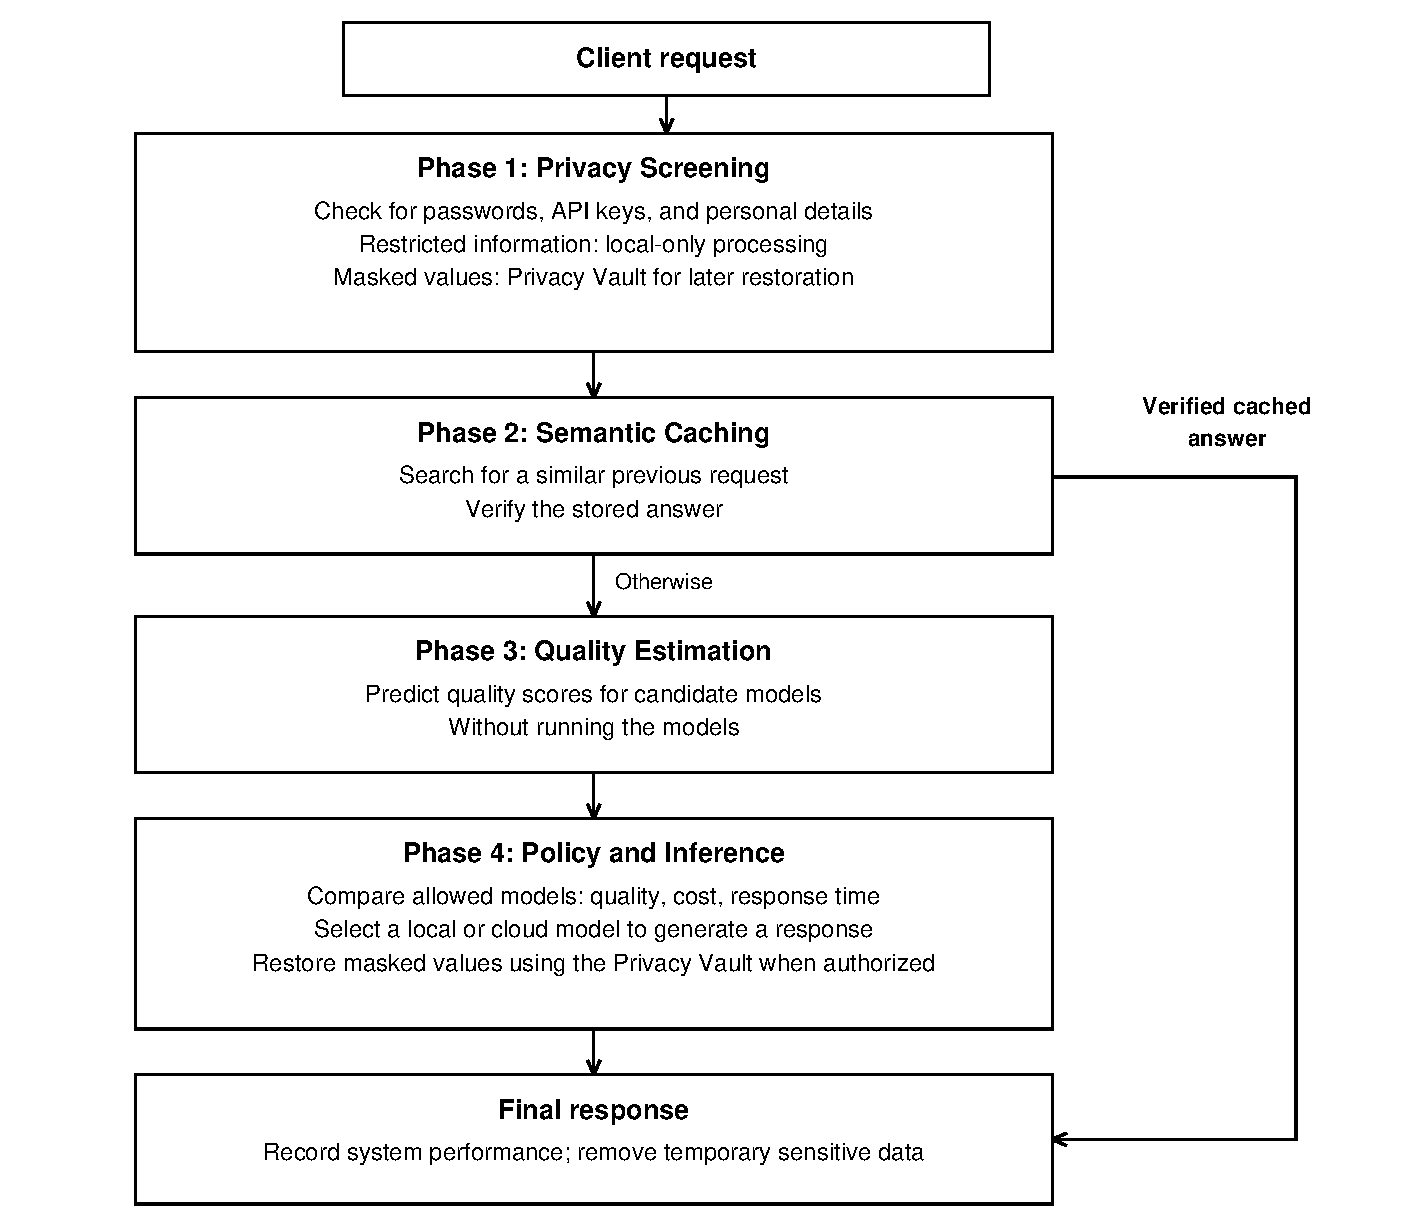
\includegraphics[width=0.98\textwidth]{Figures/pipeline_final.pdf}
\caption{Proposed four-phase request processing pipeline of AetherFlow.}
\label{fig:pipeline_arch}
\end{figure}

The gateway first checks the request for sensitive information, such as passwords, API keys, and personal details. Requests containing restricted information are marked for local-only processing. When masking is allowed, sensitive values are replaced and their original values are kept temporarily in the Privacy Vault. The gateway then searches for a similar previous request. If a stored answer is found and verified, it is returned directly. This avoids another model call and helps reduce response time and cost.

If no suitable stored answer is found, the quality predictor estimates how well each candidate model can answer the request without running those models. The gateway compares the allowed models using predicted quality, cost, and response time. It selects a local model for restricted requests. Other requests may use an allowed local or cloud model. The selected model generates the response. Before returning it, the gateway restores any masked values using the Privacy Vault when authorized. It also records system performance and removes temporary sensitive data. Figure~\ref{fig:system_arch} shows how the system components are connected.
\section{Design Considerations}

This section explains the main factors considered while designing AetherFlow. These include system requirements, limitations, security, performance, and development methods.

\subsection{Assumptions and Dependencies}

AetherFlow depends on local LLMs, cloud APIs, and supporting services. The system assumes that all required services are properly configured before use. Local models need suitable hardware, while cloud models require an internet connection and valid API keys provided by the user. The gateway also depends on predefined model configurations and routing policies. These settings help the system decide how requests should be processed. The initial design focuses on a limited number of local and cloud models rather than supporting every available LLM provider.

\subsection{General Constraints}

The design of AetherFlow considers limitations related to hardware, software, available resources, communication, and security.

\subsubsection{Hardware and Software Environment}

AetherFlow uses FastAPI and Uvicorn to handle incoming requests. Local LLMs are served through vLLM or Ollama. Running these models requires sufficient RAM and GPU resources, depending on the model size. The proposed system uses Qwen3-8B and Llama-3.1-8B-Instruct as local models. The system is designed to work within the available hardware rather than requiring expensive infrastructure. Model performance may vary depending on the computer's specifications and the number of requests being processed.

\subsubsection{End-User Environment}

The main client application for AetherFlow is a VS Code extension. It allows developers to send prompts and perform tasks such as explaining code, fixing errors, refactoring code, and generating tests. Users can interact with the system through a chat interface without selecting a model for every request. The extension sends requests to the gateway and displays the generated responses. The current prototype uses a mock backend for testing. In the proposed system, the extension will communicate with the actual AetherFlow gateway.

\subsubsection{Availability of Resources}

The availability of models depends on local hardware and external cloud services. Local models may become slow when GPU resources are busy or several requests are being processed together. Cloud models depend on the internet connection, provider availability, and API usage limits. These conditions may affect how quickly a request is completed. The gateway is designed to consider the availability of its configured models before sending a request. This helps avoid unnecessary delays when a particular model cannot handle a request.

\subsubsection{Interoperability Requirements}

AetherFlow is designed to work with different LLM providers through a common API. It follows the OpenAI-style chat-completions format so that client applications can communicate with the gateway easily. Local and cloud providers may use different request and response formats. To handle these differences, the gateway uses separate provider adapters. Each adapter manages communication with its model provider. This allows the client to use the gateway without dealing with the details of individual model APIs.

\subsubsection{Interface and Protocol Requirements}

The gateway communicates with client applications using HTTP APIs, with request and response data exchanged in JSON format. It also plans to support Server-Sent Events (SSE) for streaming responses. Streaming allows users to see the generated answer gradually instead of waiting for the entire response. HTTPS will be used where secure communication is required. These interfaces provide a common way for the VS Code extension and other supported applications to send requests and receive results.

\subsubsection{Data Repository and Distribution Requirements}

AetherFlow uses PostgreSQL and Qdrant for different storage purposes. PostgreSQL stores model configurations, routing policies, and request usage records. These records also support the dashboard by providing information about model usage, cost, and response time. Qdrant is used for semantic caching. It stores query embeddings and approved cache entries so the gateway can search for similar previous requests. The local Privacy Vault is kept separate from these databases and handles temporary sensitive data mappings.

\subsubsection{Security Requirements}

AetherFlow requires proper access control and protection of sensitive information. The gateway checks incoming requests for private data before allowing them to reach a model. Requests containing restricted information must remain within the local environment. Cloud API keys are protected and are not included in normal request logs. The system also limits access to configuration settings and stored records. These measures help prevent unauthorized use of the gateway and reduce the risk of exposing private information.

\subsubsection{Performance Requirements}

The main performance goal is to reduce response time and unnecessary processing costs. The project targets a response time below 200 ms for cached requests and aims to keep policy decision overhead below 15 ms. These are proposed targets that will be checked during testing. The system will also measure cache hit rate, total response time, and model usage cost. Performance testing will help determine whether the gateway improves efficiency compared with using a single model for every request.

\subsection{Goals and Guidelines}

The system design follows guidelines that make AetherFlow easier to develop, test, maintain, and extend.

\subsubsection{Loose Coupling}

AetherFlow is divided into separate components that communicate through defined interfaces. Each component performs its own task without depending heavily on the internal code of other components. For example, the quality predictor produces model scores, while the policy engine uses those scores to make routing decisions. This separation allows developers to test and update one component without changing the entire system. It also makes debugging easier because problems can be traced to the component responsible for a particular task.

\subsubsection{Non-blocking Asynchronous I/O}

The gateway uses asynchronous processing to handle requests efficiently. Some operations, such as cloud API calls and database queries, involve waiting for external services. During this waiting time, the gateway can continue handling other requests instead of blocking them. FastAPI provides support for this approach. More demanding tasks, such as local model inference, need separate processing resources. This design is useful when multiple clients are using the gateway at the same time and helps the system remain responsive.

\subsubsection{Privacy by Design}

Privacy protection is included in the main request processing flow rather than being handled only at the end. The Privacy Analyzer identifies sensitive information and applies the required rules. When masking is needed, sensitive values are replaced with placeholders. Their original values are temporarily stored in the local Privacy Vault and can be restored for an authorized client. Restricted requests are processed locally, even if masking has been applied. Temporary mappings are removed after processing and are not stored in general system logs.

\subsubsection{Extensibility}

The initial version of AetherFlow supports a predefined set of local and cloud models. However, the architecture allows more models to be added in the future. New providers can be connected through adapters without changing the main gateway structure. Their configurations and quality prediction support must also be updated before they can be used for routing. This makes it possible to expand the system gradually while keeping the existing request processing flow unchanged.

\subsubsection{Responsiveness}

The gateway aims to provide a smooth experience for users. When a request is answered through the semantic cache, the system can return the result without generating a new response. For requests that require inference, the selected model generates the answer, which can be streamed to the client as it becomes available. This allows users to see progress instead of waiting for the full response. Actual response time will still depend on the selected model, prompt length, and network conditions.

\subsection{Development Techniques}

AetherFlow follows a component-based development approach. The main components are developed and tested separately before being connected into the complete gateway. Development includes privacy screening, semantic caching, quality estimation, model routing, and the supporting APIs. After individual testing, integration tests will check whether requests move correctly through the system.

Git and GitHub are used for version control and team collaboration. The VS Code extension serves as the reference client for demonstrating the project. The current mock workflow supports initial testing, while the completed gateway will be evaluated using actual model responses and benchmark datasets.

\section{System Architecture}

AetherFlow is divided into three main parts: the client, the gateway, and the LLM services. The client sends requests to the gateway, which processes them and communicates with the selected model. The gateway also connects to supporting services for privacy checking, caching, and storing system information.

Figure~\ref{fig:system_arch} shows the proposed architecture. The VS Code extension acts as the main client, while the administrator uses a dashboard to manage settings and monitor performance. The FastAPI gateway connects the different components. Local models run within the protected environment, while cloud models are accessed through their APIs. Requests containing restricted information remain within the local system.

\begin{figure}[!p]
\centering
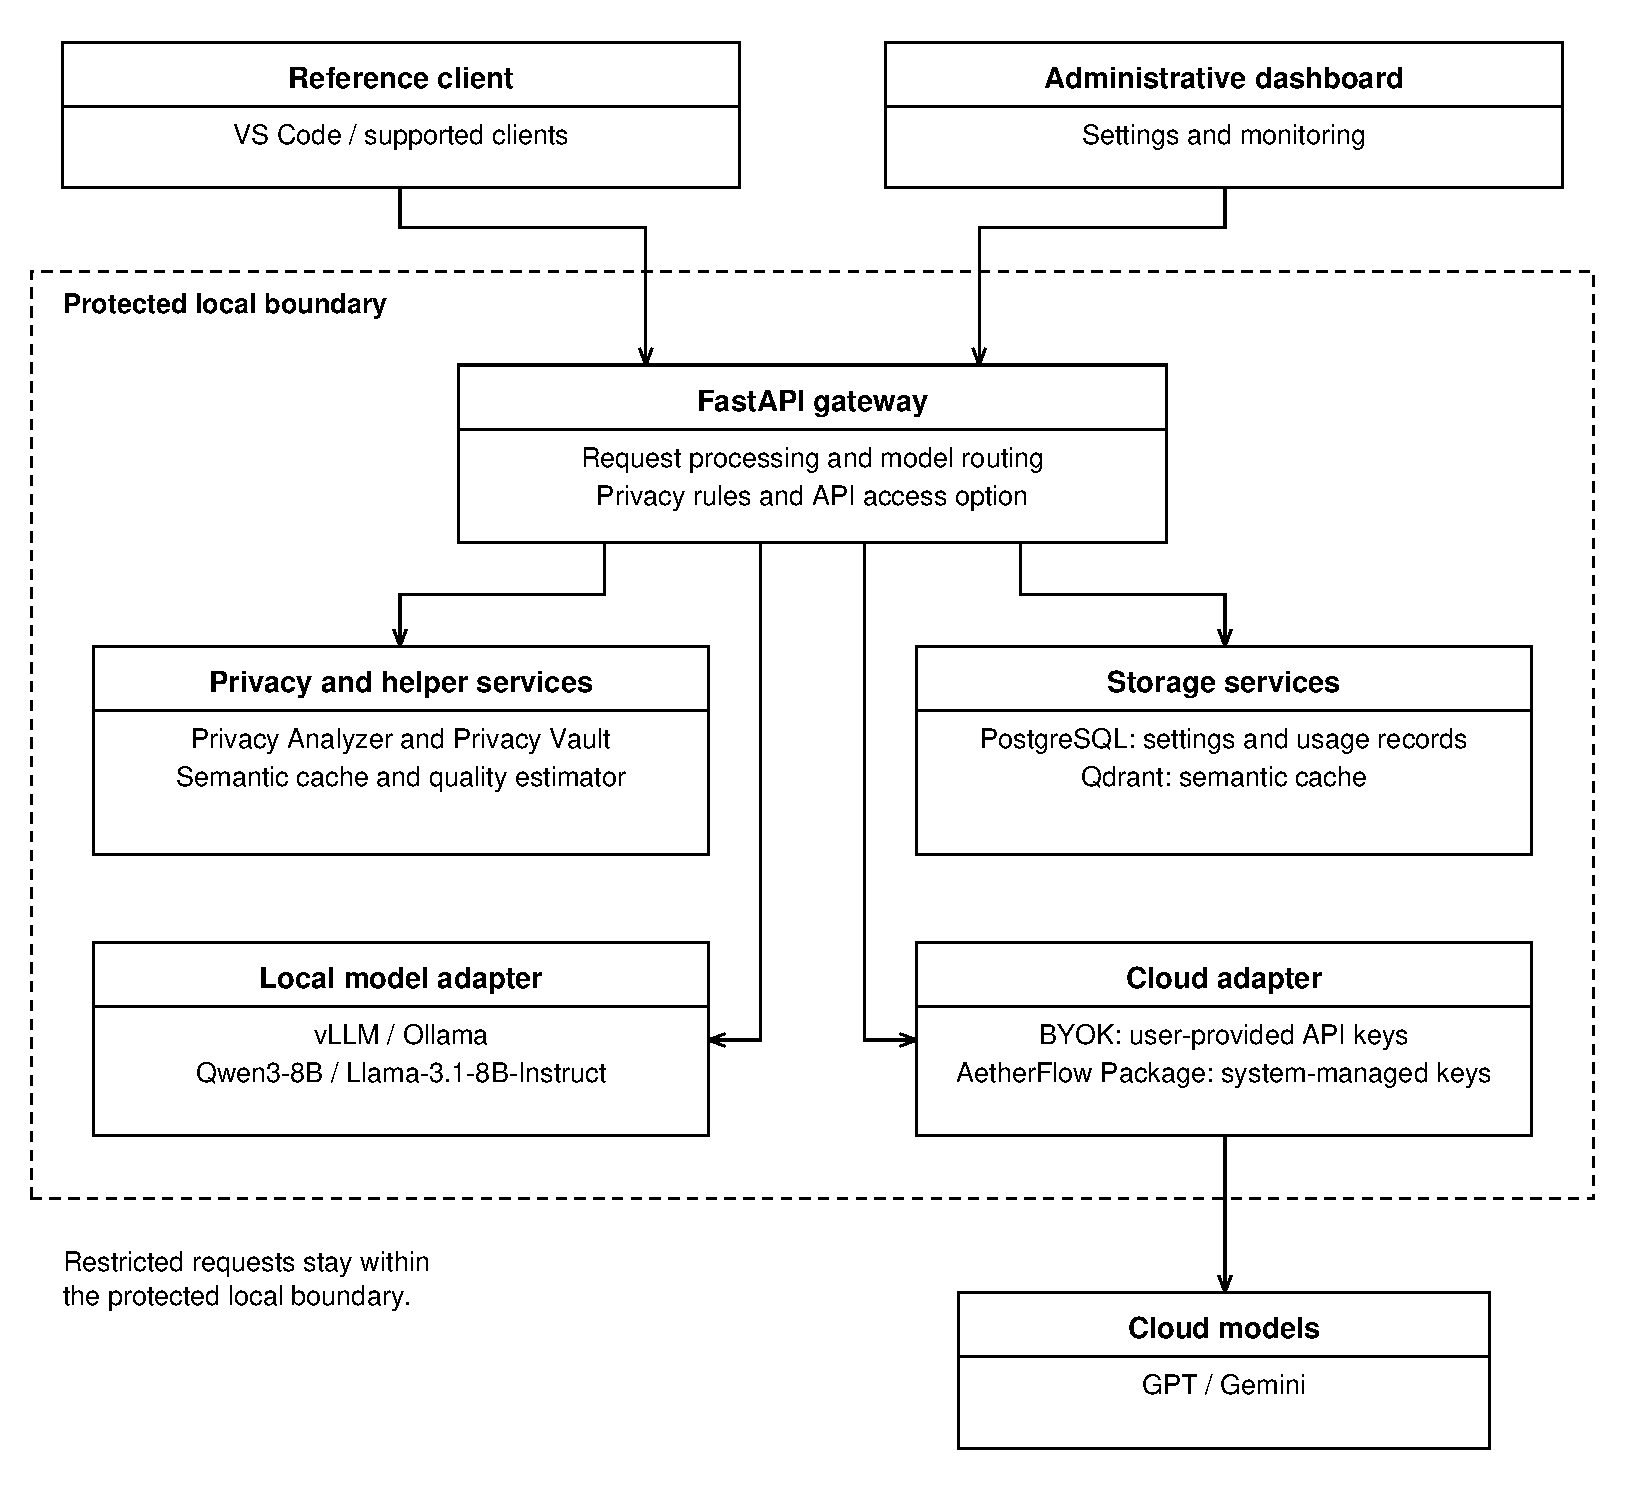
\includegraphics[width=0.98\textwidth]{Figures/system_final.pdf}
\caption{Proposed AetherFlow architecture with local and cloud model access.}
\label{fig:system_arch}
\end{figure}

\subsection{Subsystem Architecture}
\label{sec:subsystem_arch}

The gateway is divided into smaller subsystems, with each subsystem performing a specific task. The FastAPI gateway receives requests from the client and manages their processing. It also checks client access and connects the different components of the system.

The Privacy Analyzer checks requests for sensitive information. If restricted information is found, the request is marked for local-only processing. When masking is required, sensitive values are replaced with placeholders. Their original values are temporarily stored in the encrypted Privacy Vault and can be restored when authorized.

The semantic cache checks whether a similar request has already been answered. Qdrant is used to find similar previous requests, while a cross-encoder checks whether the stored answer is suitable for the current request. If a valid answer is found, it is returned directly. Otherwise, the request continues to quality estimation.

The quality estimator uses a trained DistilDeBERTa model to predict how well each supported LLM can answer the request. It produces quality scores without running the models. The policy engine then uses these scores along with cost, response time, and privacy rules to select a model from the predefined local and cloud models.

After model selection, the gateway sends the request through the appropriate model adapter. Local models are accessed through vLLM or Ollama, while cloud models are accessed through their APIs. For cloud access, the system supports two proposed options. In Bring Your Own Key (BYOK), users provide their own API keys. In the AetherFlow Package, the gateway uses API keys managed by the system. Both options follow the same privacy and routing rules.

The selected model generates a response, which is returned to the client. The system also records information such as model usage, cost, and response time. The administrator can view this information through the dashboard and update routing settings.

\begin{table}[!htbp]
\centering\small
\begin{tabularx}{\textwidth}{|P{3.4cm}|X|X|}\hline
\textbf{Component / interface} & \textbf{Input} & \textbf{Output}\\\hline
Client API & Prompt or code, request settings, API access option & Final answer or response stream\\\hline
Administrator dashboard & Model settings, routing rules, package key settings & Usage, cost, and response time\\\hline
Privacy Analyzer and Vault & Request and privacy rules & Checked request, temporary mappings, restored values\\\hline
Semantic cache & Approved request & Verified stored answer or no suitable answer\\\hline
Quality estimator & Request and supported model list & Predicted quality scores\\\hline
Policy engine & Scores, privacy rules, cost, response time & Selected allowed model\\\hline
Model adapters & Approved request and selected API key for cloud access & Model response and usage information\\\hline
\end{tabularx}
\caption{Main subsystem interfaces and the information they exchange.}
\label{tab:interfaces}
\end{table}

\subsection{Data Flow Diagrams}
\label{sec:data_flow_diagrams}

Data Flow Diagrams (DFDs) show how information moves through AetherFlow. They explain how requests enter the gateway, how different components process the data, and how responses are returned to the client. The system uses Level 0 and Level 1 DFDs to explain the overall flow and internal processing.

\subsubsection{Level 0 DFD - Context Diagram}
\label{sec:dfd_level0}

The Level 0 DFD shows AetherFlow as a single system and its communication with external entities. As shown in Figure~\ref{fig:dfd_level0}, the main entities are the developer client, enterprise administrator, local LLM service, and cloud LLM provider.

The developer sends prompts or code through the VS Code extension or another supported client. The user can choose between two cloud API access options. In BYOK mode, the user provides their own API keys. In the AetherFlow Package option, cloud access is provided through system-managed API keys. The selected access option is sent to the gateway along with the request settings.

The administrator manages model configurations, routing policies, and system settings through the dashboard. The gateway communicates with local or cloud models based on the routing decision and returns the generated response to the client. Restricted requests are processed locally, regardless of the selected API access option.

\begin{figure}[!htbp]
\centering
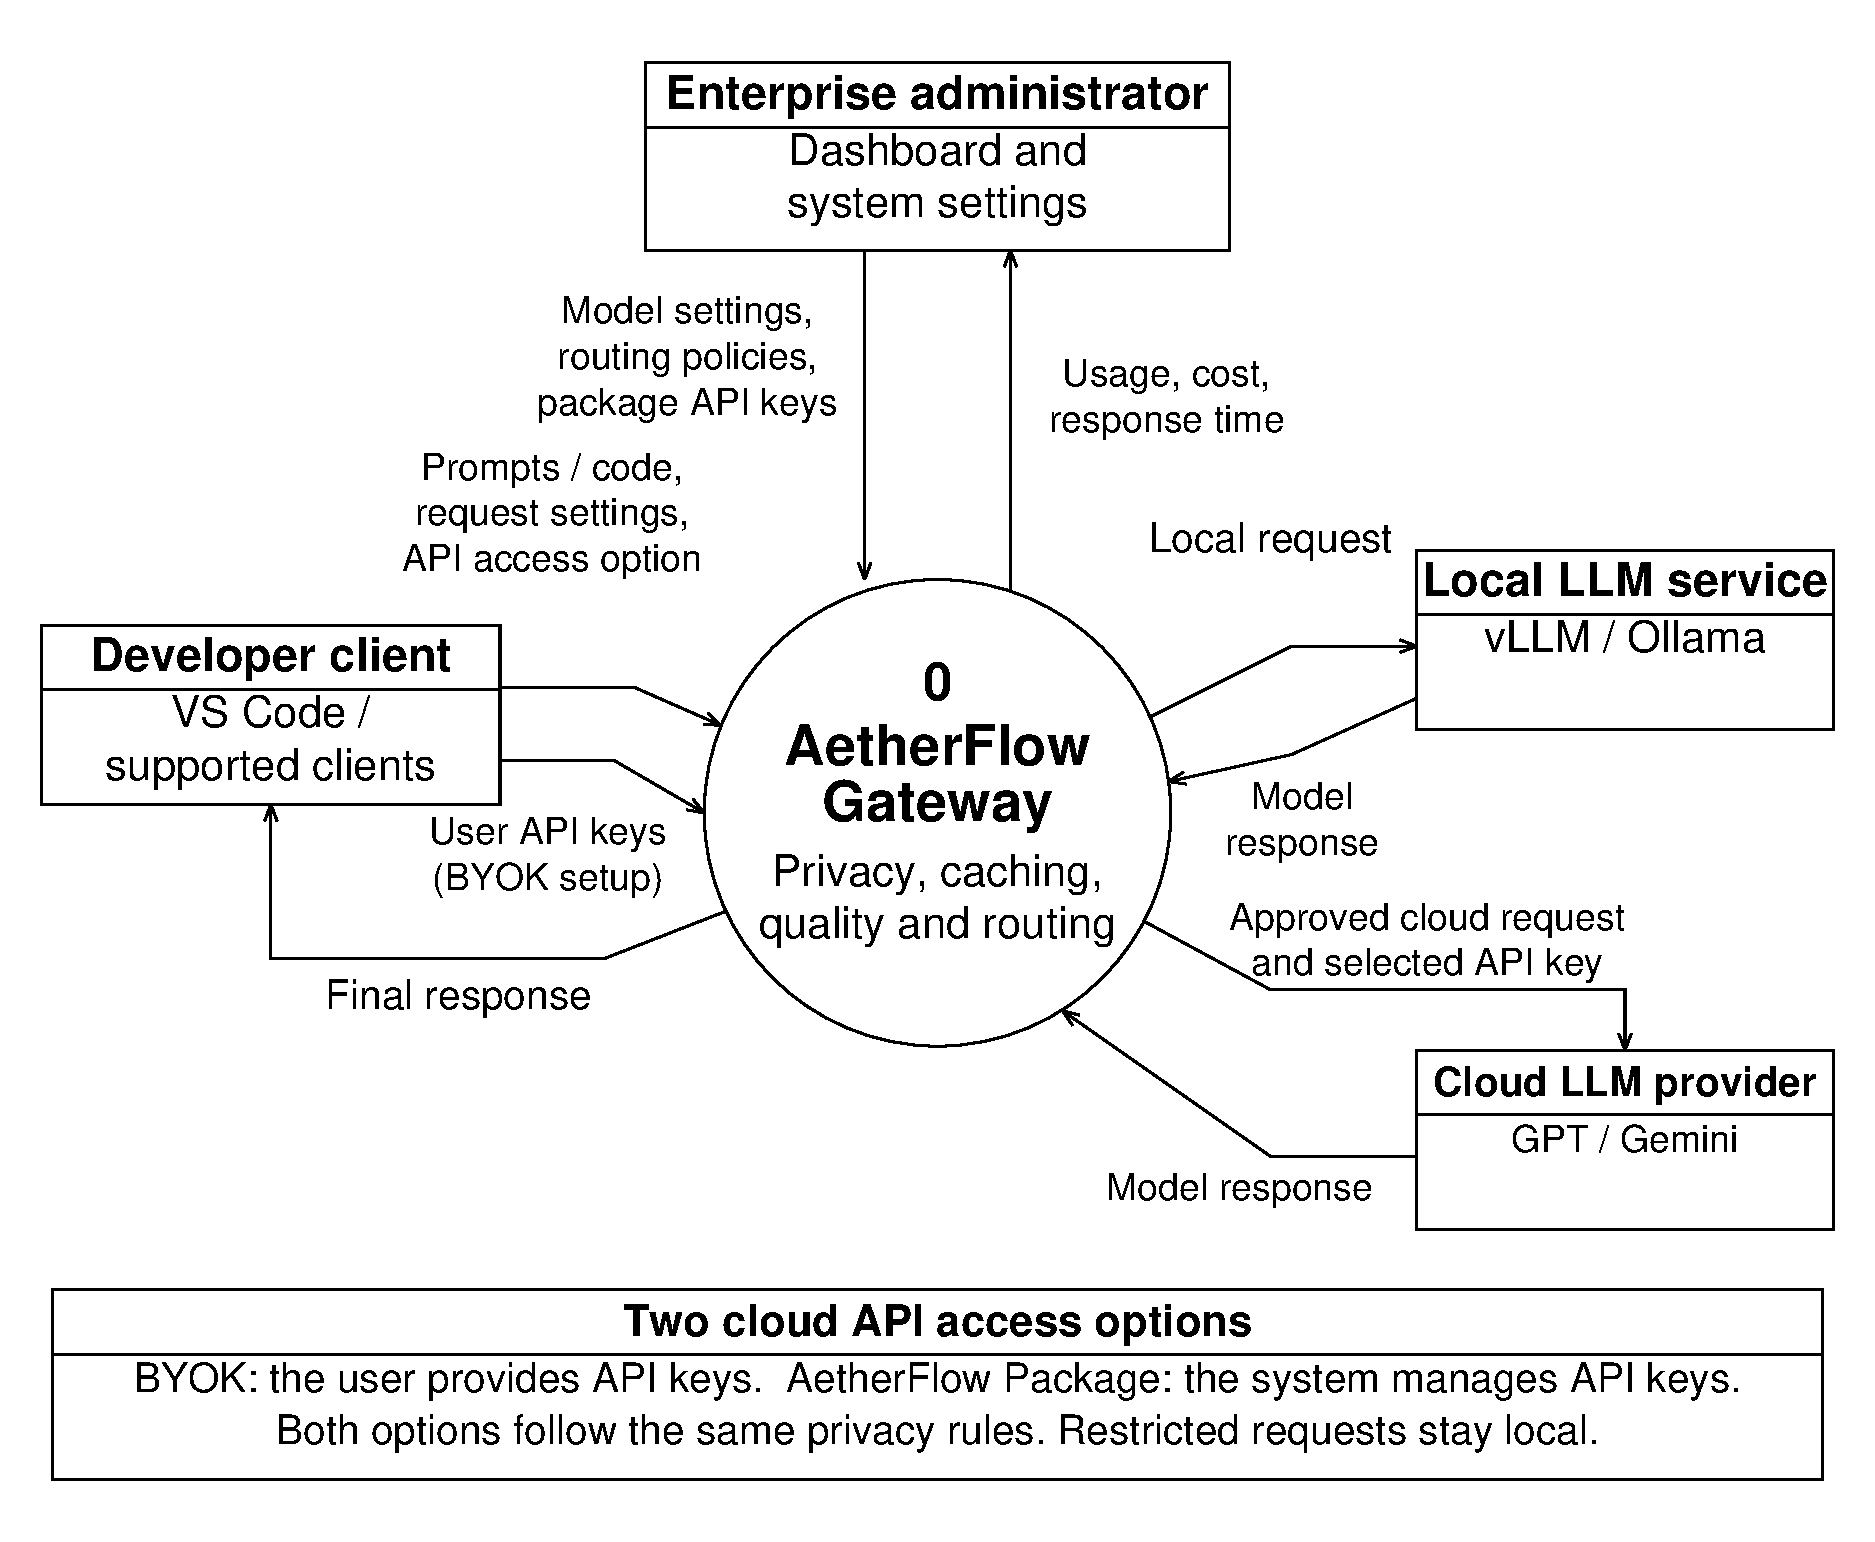
\includegraphics[width=0.98\textwidth]{Figures/dfd_level0.pdf}
\caption{Level 0 DFD showing external interfaces and both cloud API access options.}
\label{fig:dfd_level0}
\end{figure}

\subsubsection{Level 1 DFD - Detailed Data Flow}
\label{sec:dfd_level1}

The Level 1 DFD uses the same four external interfaces as the Level 0 DFD: the developer client, enterprise administrator, local LLM service, and cloud LLM provider. The circles show internal processes, while the parallel lines show data stores. BYOK and the AetherFlow Package are two access options within the system, not separate external interfaces. The diagram shows how a request is processed inside the gateway. As shown in Figure~\ref{fig:dfd_level1}, the request first passes through privacy screening, where sensitive information is identified. If masking is required, sensitive values are replaced with placeholders, and their original values are stored temporarily in the Privacy Vault.

The request then moves to the semantic cache, where Qdrant searches for similar previous requests. If a suitable cached answer is found and verified, it is returned directly. Otherwise, the quality estimator predicts scores for the supported models. The policy engine uses these scores along with cost, latency, and privacy rules to select a model.

After model selection, the gateway checks the API access option if a cloud model is selected. For BYOK, it uses the user's stored API key. For the AetherFlow Package, it uses the system-managed API key. API keys are stored securely and are only used when communicating with the selected cloud provider. User keys and system-managed keys are kept in a separate secure API-key store. They are not stored in the Privacy Vault, semantic cache, or general request logs. If a local model is selected, no cloud API key is required.

The selected model processes the request and returns its response to the gateway. The gateway prepares the final answer and sends it to the client. PostgreSQL stores system settings and usage records, Qdrant stores semantic cache data, and the Privacy Vault stores temporary sensitive mappings.

\begin{figure}[!p]
\centering
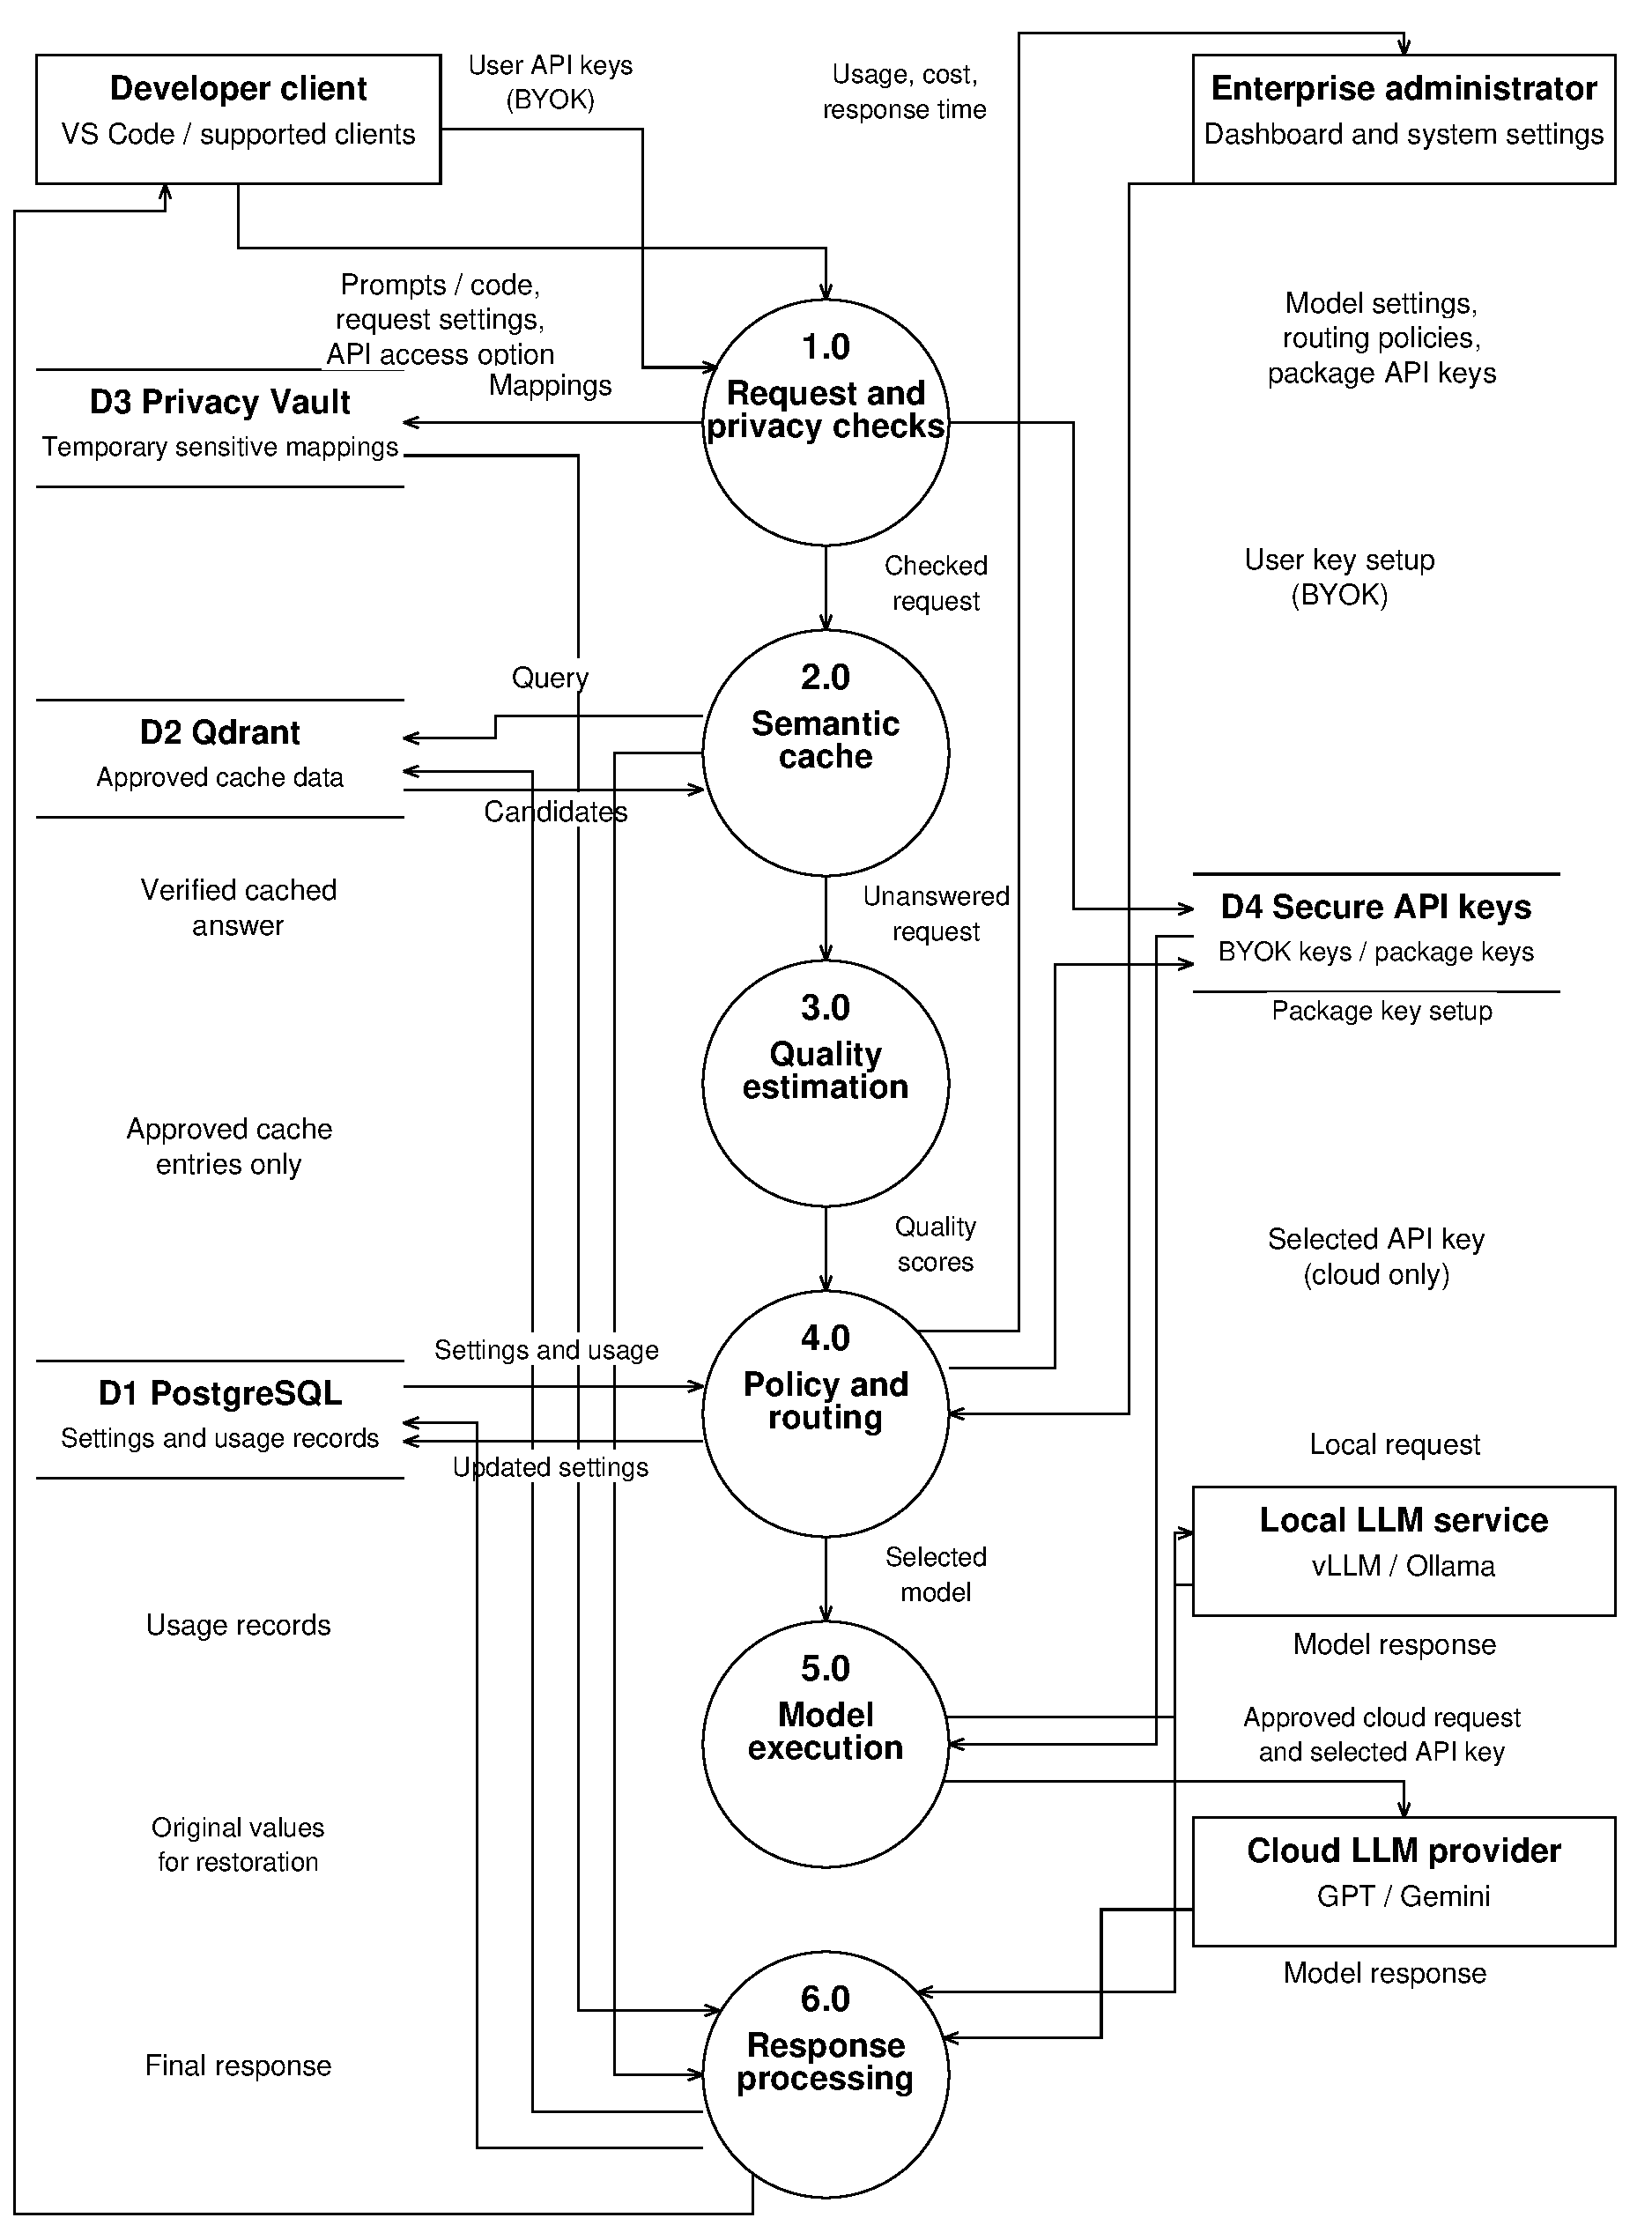
\includegraphics[width=0.98\textwidth]{Figures/dfd_level1.pdf}
\caption{Level 1 DFD with the same four external interfaces as Level 0.}
\label{fig:dfd_level1}
\end{figure}

\section{Architectural Strategies}

This section explains the main strategies used in designing AetherFlow. These strategies were selected to make the system efficient, secure, and easy to maintain. They also help the gateway support different LLM providers and handle multiple requests.

\subsection{Asynchronous Processing}

AetherFlow uses FastAPI with Python to handle incoming requests. The gateway follows an asynchronous approach, which allows it to handle other requests while waiting for database operations or cloud API responses. In a synchronous system, a request may keep a worker busy while waiting for an external service. Asynchronous processing reduces this problem and makes better use of available resources.

Tasks such as privacy analysis and quality prediction require more processing power. These tasks are planned to run in separate workers so they do not block the main gateway. This approach was chosen to support multiple users without requiring a separate gateway process for every request.

\subsection{Modular Architecture and Model Adapters}

AetherFlow follows a modular design where different components have separate responsibilities. The gateway connects these components through defined interfaces. This allows individual components to be developed, tested, and updated without changing the entire system.

The system also uses model adapters to communicate with different LLM providers. Instead of writing provider-specific code directly inside the gateway, each adapter handles communication with its provider. This approach was chosen because local and cloud models may use different APIs. It also makes it easier to add new models in the future without making major changes to the gateway.

\subsection{Privacy and Local Processing}

AetherFlow uses a protected local environment to handle restricted information. This approach was chosen because sending every request to cloud providers could expose sensitive data to external services. Local processing gives the organization more control over how its private information is handled.

The gateway also supports masking and temporary storage of sensitive values in the Privacy Vault. However, masking does not automatically make a restricted request safe for cloud processing. Using local models may require more hardware resources, but it helps maintain privacy. The system gives privacy rules priority over cost and response time when selecting a model.

\subsection{Concurrency and Resource Management}

AetherFlow is designed to process requests from multiple users at the same time. Since these requests may share resources such as model capacity and usage budgets, the gateway needs a way to manage them safely.

The proposed design uses PostgreSQL transactions and locking to prevent conflicts when shared records are updated. For example, two requests should not be allowed to use the same remaining budget without checking the updated usage. Database transactions were chosen instead of relying only on memory-based locks because the gateway may use multiple workers. This helps maintain correct usage records and prevents conflicts between requests.

\subsection{Data Storage Strategy}

AetherFlow uses separate storage systems based on the type of data being handled. PostgreSQL is selected for structured records such as model configurations, routing policies, and usage information. Qdrant is selected for semantic caching because it supports searching for queries with similar meanings.

Using only a relational database for all operations was not selected because semantic similarity search has different requirements from normal record storage. The Privacy Vault is also kept separate to protect temporary sensitive mappings. This approach allows each storage component to handle the type of data it is designed for.

\subsection{Error Handling and Recovery}

AetherFlow must handle problems such as unavailable models, failed API calls, and database connection issues. The gateway is designed to return a clear error message when a request cannot be completed.

For temporary provider failures, the system may retry the request using another allowed model. However, the replacement model must still follow the original privacy rules. Restricted requests cannot be moved to cloud models simply because a local model is unavailable. This approach was chosen to improve reliability without compromising privacy. The gateway also avoids unnecessary repeated requests that could increase cost and response time.

\section{Domain Model and Class Diagram}

The class diagram shows the main classes of AetherFlow and how they interact. Figure~\ref{fig:class_diagram} presents the proposed class structure of the gateway.

The GatewayProxy is the main class that manages incoming requests. It creates a RequestContext to store information about each request, such as its privacy status and selected settings. The gateway then uses different services to process the request.

The PrivacyAnalyzer checks for sensitive information and uses the TokenVault when masking is required. The SemanticCache searches for previous answers, while the QualityEstimator predicts the response quality of supported models. The ExecutionPolicyEngine uses these predictions along with cost, latency, and privacy rules to select a model. The UsageLedger checks the available budget, reserves an amount before a model call, records actual usage, and releases any unused reserved amount.

The ModelAdapter provides a common interface for model communication. LocalModelAdapter connects to local models through vLLM or Ollama, while CloudModelAdapter connects to supported cloud APIs. CloudModelAdapter chooses the appropriate API key: the user-provided key for BYOK or a system-managed key for the AetherFlow Package. This structure allows different models to work with the same gateway.

\begin{figure}[!p]
\centering
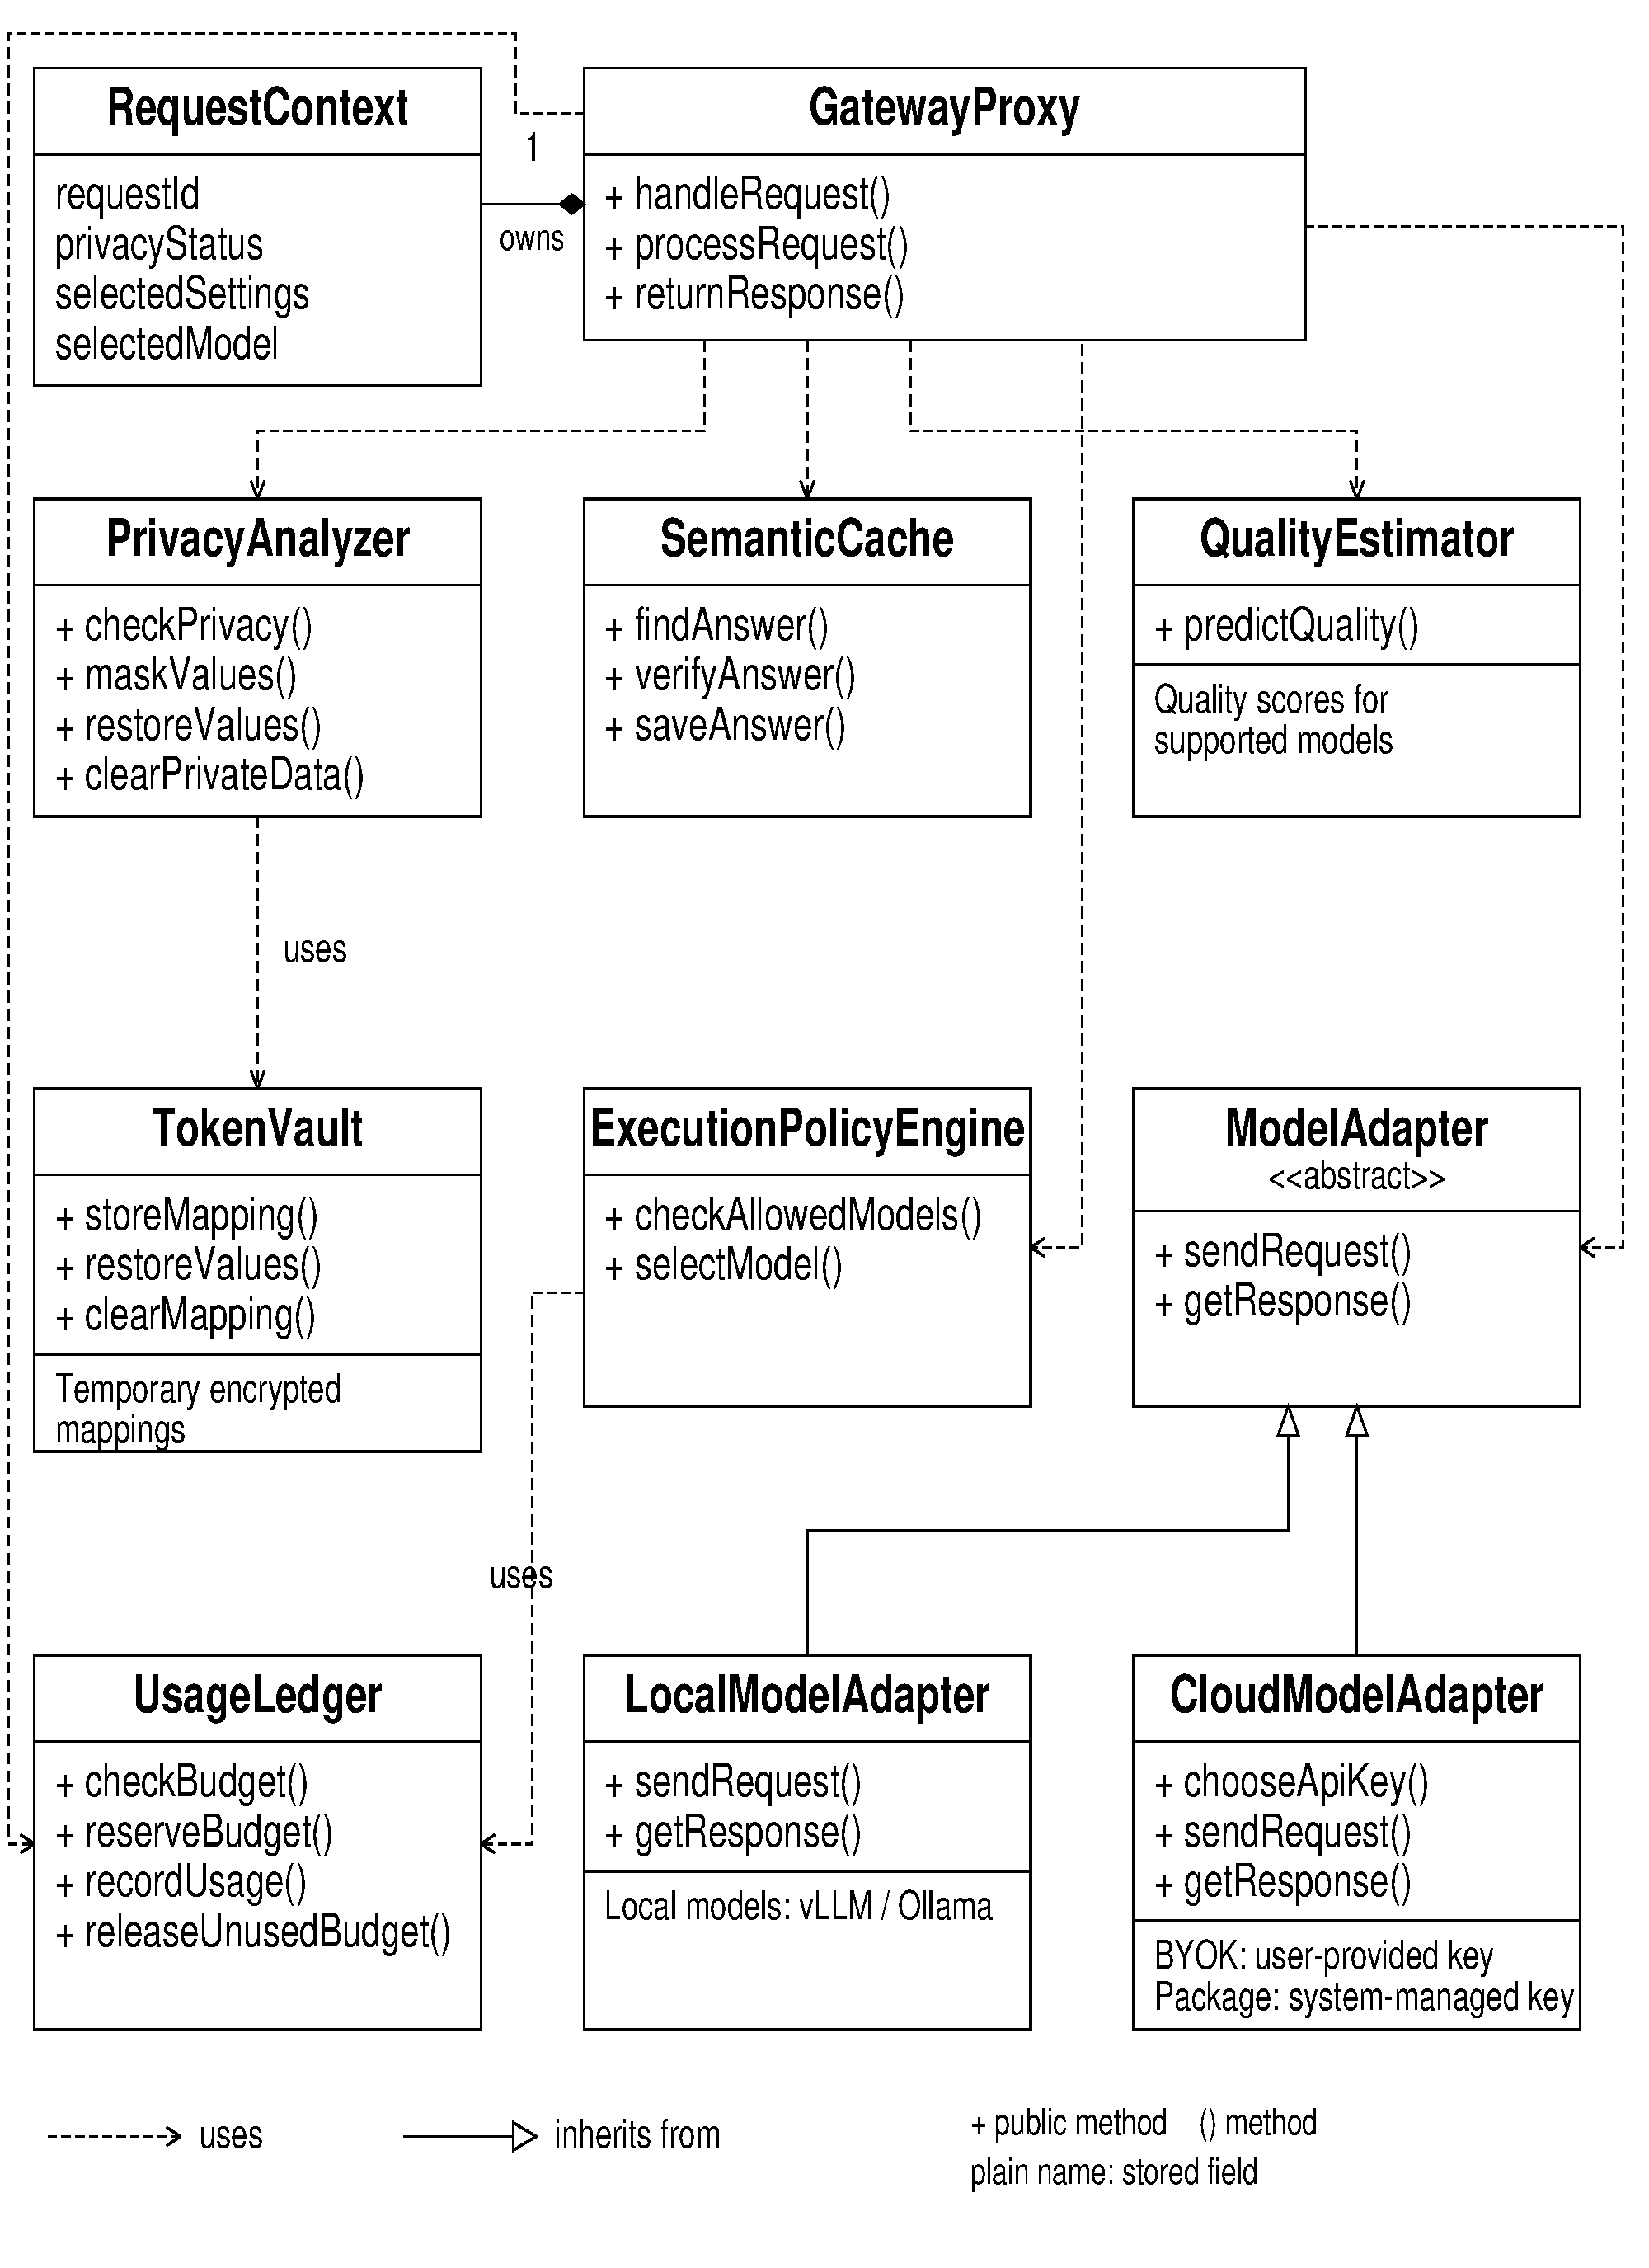
\includegraphics[width=\textwidth,height=0.92\textheight,keepaspectratio]{Figures/class_final.pdf}
\caption{Simplified proposed class structure of the AetherFlow gateway.}
\label{fig:class_diagram}
\label{fig:class_diag}
\end{figure}

\subsection*{Sequence Diagram}

The sequence diagram shows how the different components communicate when processing a request. The PrivacyAnalyzer uses the TokenVault for temporary mappings. The ExecutionPolicyEngine uses the UsageLedger for budget checks and usage records. Figure~\ref{fig:sequence_diagram} presents the proposed request flow.

The client first sends a request to the gateway. The PrivacyAnalyzer checks for sensitive information and applies masking when required. The gateway then checks the semantic cache for a verified previous answer when caching is allowed. If a suitable answer is found, it is returned directly.

Otherwise, the QualityEstimator predicts quality scores for the supported models. The ExecutionPolicyEngine compares the allowed models based on quality, cost, and latency. The gateway then sends the request through the selected model adapter and receives the generated response.

Before sending the final answer, the gateway restores masked values when authorized. It also records usage information and removes temporary sensitive mappings. These steps complete the request processing flow.

\begin{figure}[!htbp]
\centering
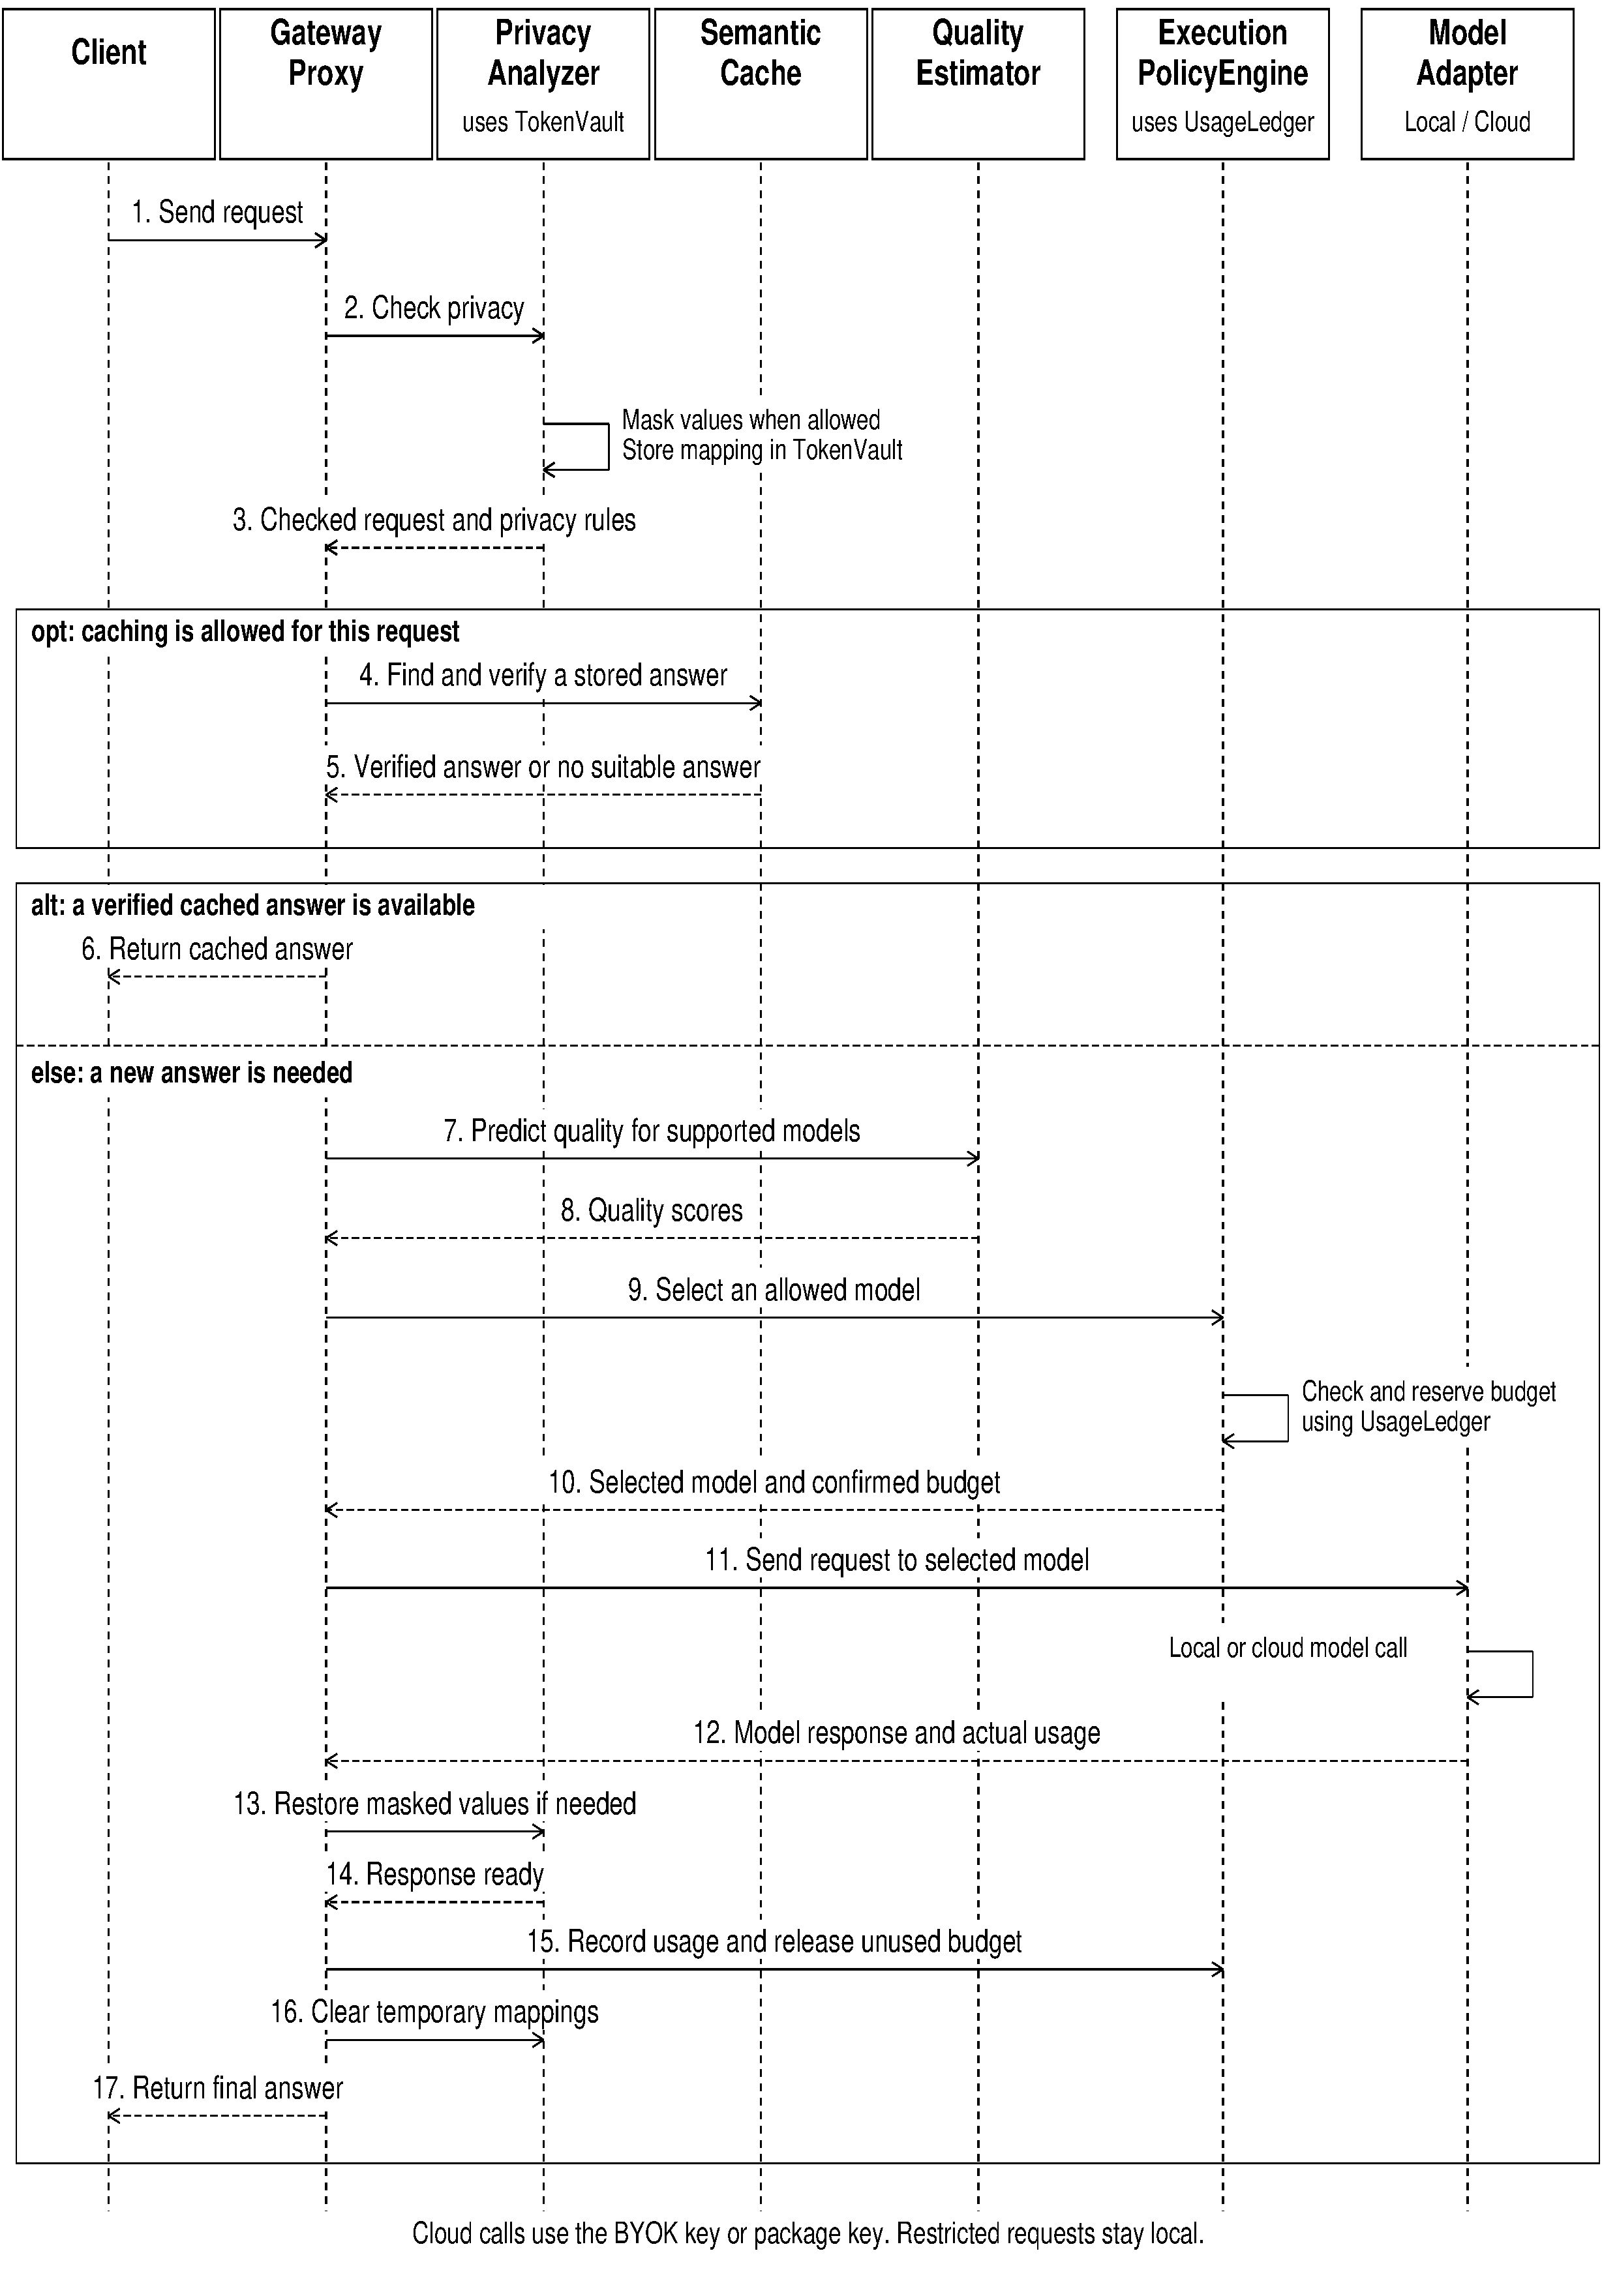
\includegraphics[width=\textwidth,height=0.92\textheight,keepaspectratio]{Figures/sequence_final.pdf}
\caption{Simplified proposed request processing sequence of AetherFlow.}
\label{fig:sequence_diagram}
\label{fig:seq_diag}
\end{figure}

\section{Policies and Tactics}
\label{sec:policies}

This section explains the coding, testing, deployment, and maintenance practices planned for AetherFlow. These practices help keep the system organized, reliable, and easier to manage during development.

\subsection{Conventions and Coding Guidelines}

AetherFlow is developed mainly using Python for the backend and TypeScript for the VS Code extension. The code is organized into separate modules for privacy screening, semantic caching, quality estimation, model routing, and API communication. Each module is responsible for a specific task, making the code easier to understand and maintain.

The project follows consistent naming rules, clear function names, and proper error handling. Important functions include comments where needed. Git and GitHub are used to manage code changes and support team collaboration. API keys, passwords, and sensitive user information are not stored directly in the source code or normal logs.

\subsection{Testing Approaches}

AetherFlow uses different testing methods to check whether the system works correctly. Unit testing is planned for individual components such as the Privacy Analyzer, semantic cache, quality predictor, and policy engine. These tests check whether each component produces the expected result.

Integration testing checks how components work together when processing a request. For example, it verifies that restricted requests are handled locally and that cached answers are returned only after verification. The VS Code extension is also tested to check communication with the gateway.

The completed system will be evaluated using benchmark datasets such as MMLU, GSM8K, HumanEval, and MT-Bench. Testing will focus on response quality, cost, latency, and privacy. This approach was chosen because testing individual components alone cannot confirm that the complete system works correctly.

\subsection{Continuous Integration and Deployment}

AetherFlow is planned to use Docker Compose to run the gateway and supporting services. This includes FastAPI, PostgreSQL, Qdrant, and the configured local model service. Docker Compose was selected because it makes it easier to manage multiple services in one development environment without installing and configuring each service separately.

GitHub is used for version control and collaboration. A CI workflow may be added using GitHub Actions to run basic checks and tests when code changes are pushed. This can help identify problems before new changes are merged into the main project. The initial deployment focuses on a local development environment rather than a large production setup.

\subsection{Error Handling and Recovery}

AetherFlow uses error handling to manage problems that may occur during request processing. These include invalid requests, unavailable models, failed cloud API calls, and database connection problems. The gateway returns a clear error message so the client knows that the request could not be completed.

For temporary model or provider failures, the gateway may retry using another allowed model. However, the new model must follow the same privacy rules. Restricted requests cannot be sent to cloud models as a fallback. Retry attempts are limited to avoid unnecessary delays and costs. This approach helps the system recover from temporary problems without repeating requests continuously.

\subsection{Database Management}

AetherFlow uses PostgreSQL for structured information such as model settings, routing policies, and usage records. Qdrant is used to store query embeddings and approved cache entries for semantic similarity searches. These databases have separate purposes and are accessed through the gateway's supporting services.

Database operations are designed to keep stored records consistent when multiple requests are processed. Database migrations are planned to manage changes to table structures during development. Regular backups may also be used for important system records. Sensitive mappings stored in the Privacy Vault are temporary and are not included in normal database backups. This helps protect private information while keeping the required system data available.

\section{Conclusion}
This chapter defined how AetherFlow's components will work together, from receiving a developer's request to returning an answer. The architecture, data flows, class structure, and interaction sequence provide a clear basis for implementation. Privacy rules restrict model selection and fallback, while separate storage services support usage records and verified cache reuse. The design is ready to guide development, but its behavior must still be checked through integration and testing of the complete gateway.

\chapter{Implementation and Test Cases}
\label{ch:implementation}
The implementation of FYP-I solves the problem of selection of a language model in AetherFlow with the consideration of factors such as quality, cost, latency, and privacy that influence the selection process. The AetherFlow routing prototype is available at \url{https://aether-flow-gamma.vercel.app/}. The implementation includes a web interface, JSON routing API, and some preliminary benchmarking results. The provided benchmarking results have not been independently reproduced and cannot be considered verified performance results. The other part of FYP-II includes VS Code integration, semantic caching, temporary value protection, and usage logging.

\section{Implementation}

\subsection{Web Interface and API}
The UI is constructed using React and loads the model list, routing configuration, and sample queries. The user inputs the query, task type, and mode. The request is sent to \texttt{/api/route} endpoint by the UI. It then presents the selected model, prediction of answer quality, cost estimation, response-time information, and the rationale for selecting the model.

The API is built using FastAPI and comes with interactive documentation and an OpenAPI specification of its input/output parameters. The routing request includes the query, along with optional \texttt{query\_class}, \texttt{router}, \texttt{mode}, \texttt{threshold}, \texttt{quality\_floor}, \texttt{latency\_budget\_ms}, and \texttt{sensitive}. These parameters define the query, routing configuration, and privacy option. Input validation logic will be documented and tested independently of the gateway integration process.

\begin{table}[!htbp]
\centering\small
\caption{Public interfaces of the implemented routing demonstrator}
\renewcommand{\arraystretch}{1.20}
\setlength{\extrarowheight}{1pt}
\begin{tabular}{|P{0.30\textwidth}|P{0.60\textwidth}|}
\hline
\textbf{Endpoint} & \textbf{Role} \\ \hline
\texttt{POST /api/route} & Choose a model using Legacy routing or a selected policy mode. \\ \hline
\texttt{POST /api/sensitivity} & Check whether a query matches the current sensitive-data rules. \\ \hline
\texttt{GET /api/models} & Return the model list and reported benchmark values, which still need checking. \\ \hline
\texttt{GET /api/results} & Return early comparison results and dataset details that still need checking. \\ \hline
\texttt{GET /api/objectives} & Return policy settings and evaluation summaries that still need checking. \\ \hline
\texttt{GET /api/pareto} & Show reported model choices with different quality, cost, and speed trade-offs. The measurements still need checking. \\ \hline
\texttt{GET /api/privacy} & Return privacy settings and the models allowed for sensitive queries. \\ \hline
\end{tabular}
\label{tab:implemented_api}
\end{table}

\subsection{Model List and Query Information}
The saved model-list response dated 11 November 2026 consists of eight models: Llama-3.1-8B-Instruct, Qwen3-8B, DeepSeek-v3-0324, Gemini-2.5-Flash, GPT-4.1, Claude-Sonnet-4, Gemini-2.5-Pro, and GPT-5. The name of a model on the list means that the model is set up in the prototype. The name is no guarantee of whether the model is available and connected to respond to queries. The list of models also includes cost, response time, and accuracy metrics for each task type. These metrics have not been independently verified.

There are five task types used in the prototype: Coding, Competitive Math, General Knowledge, Mathematical Reasoning, and Scientific Questionnaire. The routing response includes estimated task type, probability of the query being easy, medium, or hard, and probability of getting a correct response for each model. This information helps in selecting a model prior to sending the query to a model. Information about training and scoring adjustment procedure are included in the API documentation; however, the source code, the weights of the trained model, the dataset, and the logs have not been independently verified.

\subsection{Legacy Model Selection}
Legacy routing compares each model's predicted chance of answering correctly with a configured confidence requirement. If no candidate meets that requirement, the service returns its configured fallback model. The response includes the selected model, the fallback flag, predicted scores, and reasons for the decision. These fields describe the prototype's selection output; they do not establish that the selected model generated a correct answer. The preliminary observations are discussed in Chapter~\ref{ch:results}.

\subsection{Routing Modes}
The second router can handle Economy, Balanced, Speed, Quality, and Private modes. The request picks the router with \texttt{router=multi\_objective}, along with a necessary mode. Economy mode pays attention to cost more. Balanced mode takes into account both cost and speed. Speed mode uses an estimate of the maximum response time. Quality mode is oriented at predicted correctness. The Private mode permits only those models which meet the privacy configuration requirements.

The configurations include weights for cost and response time significance. They also include scales and adjustments for measuring values in order to put various measures on the same scale and modify predicted scores. The way these values were obtained is not independently verified. Setting a quality objective does not ensure that the chosen model will have such level of accuracy. Modes described at \texttt{/api/modes} differ from the five modes at \texttt{/api/objectives}.

\subsection{Privacy Rules and Sensitive Queries}
The current configuration permits only Llama-3.1-8B-Instruct and Qwen3-8B for queries that are deemed to be sensitive. In the preliminary experiments, in both Private mode and Balanced with the query being sensitive, an allowed model was chosen. This holds for the tested requests; it does not mean that all queries or fallbacks will comply with the policy. There are six patterns and keywords in the filtering endpoint configuration. Some of the keywords include confidential, medical record, and proprietary. These guidelines offer a basic filtering process, but the detection rate of such policies has not been quantified.

The configuration may also prohibit sensitive queries and/or turn off the use of external models. Provider data retention policy is provided by the administrator and cannot confirm the actual storage of the data by the provider. Choosing an appropriate model is just a routing decision. Further analysis is required to confirm local execution of the model, no private data leakage, removal of the temporary mapping, and no logging of sensitive data.

\subsection{Returned Results and Remaining Integration}
A multi-objective routing response consists of the selected model, mode, estimated quality, routing score, estimated cost, and response-time information. It distinguishes the decision time of the router from the estimated response time of the selected model. The latter uses average values from the benchmark, not a response produced by a model in response to the request. The measurement technique and values used in the measurement have not been independently validated. Thus, the resulting value is an estimate and not a verified response time. The model name produced by the router does not indicate whether the provider was actually called.

Now the task is to integrate the selector with the FastAPI gateway and VS Code client. The gateway will validate models' authorization, retrieve a cached response if any, select a model if necessary, invoke it, and return the response. The use of PostgreSQL for logging, Qdrant for caching, the Privacy Vault, authentication of the user, and error handling are yet to be implemented.

\subsection{Request Processing Steps}
The prototype produces the routing decision for the provided query and parameters. The saved experimental responses identify the selected model and related decision fields for the supplied inputs. For Legacy routing, the service estimates model scores based on the task type and difficulty. Then, the service compares the scores with the threshold and picks a model or the default fallback one. For multi-objective routing, the service takes into account the mode and privacy, discards the inappropriate models, compares the valid candidates based on the mode parameters and gives the selected model and explanation. This is the description of the functionality that is revealed through the API; it is not validated at all levels of internal training or scoring implementations.

Privacy criteria are the requirements for the model, while cost and speed weights are preferences for comparing the allowed models. An inexpensive external model should not become allowed due to high scores. The Speed mode additionally considers an estimate of the acceptable response time. The preliminary experiments examine particular routing decisions only. There are no broader tests of failures, fallbacks and full gateway yet.

\section{Conclusion}
The FYP-I implementation provides a web interface and an API for exploring model-selection decisions. The available responses expose the configured model list, routing choices, privacy settings, and simple keyword-screening explanations. These components provide a starting point for the proposed gateway, while the training records and reported performance summaries still require independent verification. Chapter~\ref{ch:results} examines the preliminary experimental evidence. Live inference, the semantic cache, the Privacy Vault, usage logging, and VS Code integration remain work for FYP-II, together with formal integration and acceptance testing.

\clearpage


\chapter{Experimental Results and Discussion}
\label{ch:results}

This chapter describes the initial experiments carried out using the present AetherFlow routing prototype. The experiments explore issues of configuration of the model, influence of routing parameters on the selected model, and reaction of the keyword screening interface. The findings are based on the analysis of recorded API request-response pairs and will be evaluated with respect to expected functioning of the prototype. The focus of this evaluation is selection of models and interface output. The performance of answer generation and the whole gateway are not evaluated here.

\section{Experimental Setup}
The prototype was assessed by providing selected prompts with various routing configurations and analyzing the resulting output. The tests concentrated on model selection and sensitivity detection. The prompt ``Explain binary search.' was provided with the use of Legacy, Balanced, and Private modes. The artificial prompt ``This is confidential proprietary information.' was provided with the help of Balanced mode and with the parameter \texttt{sensitive=true}. This prompt was also used with the sensitivity endpoint. The saved API requests were passed via the corresponding Python script with one-time usage of every input and configuration. There are seven responses analyzed here: one model list, one privacy configuration, four routing decisions, and one sensitivity detection. No actual personal data was provided.

\section{Preliminary Experimental Results}
The experiments try to answer the following questions: if the prototype reveals the configuration required for the selection, if the settings of the routes influence the choice returned, and if the configuration of a sensitivity keyword results in the expected classification. Seven out of seven applicable requests have resulted in HTTP 200. This proves that the interfaces returned positive responses to these requests; the interpretation of their content will be done below.

\subsection{Model Configuration and Approved Destinations}
Experiment 1 retrieved the list of models and the privacy parameters. The response for model list had eight unique, non-empty model IDs. The response for privacy parameters returned two models that are approved for sensitive queries. Table~\ref{tab:prototype_configuration_results} shows the observed configuration.

\begin{table}[!htbp]
\centering\small
\setstretch{1}\renewcommand{\arraystretch}{1.15}
\caption{Observed model and privacy configuration}
\begin{tabular}{|P{0.23\textwidth}|P{0.30\textwidth}|P{0.35\textwidth}|}\hline
\textbf{Configuration} & \textbf{Recorded Result} & \textbf{Interpretation} \\ \hline
Model list & Eight distinct model identifiers were returned. & The interface exposes a defined set of model entries against which routing choices can be checked. \\ \hline
Sensitive-query approvals & Llama-3.1-8B-Instruct and Qwen3-8B were approved. & The configuration supplies an explicit allowed set for the privacy-related comparisons. \\ \hline
\end{tabular}
\label{tab:prototype_configuration_results}
\end{table}

These answers define the setup for interpreting the routing experiment. For example, a chosen identifier can be verified from the registry, and a privacy-oriented decision can be checked against the approved models. Nevertheless, a configured identifier does not confirm that a model is connected, accessible, and active in this setting. In the same way, the approval flag represents a configured rule and does not indicate anything about the provider’s handling of the data. Thus, the experiment shows a reference configuration rather than a benchmark of model capabilities or an example of its secure operation.

\subsection{Effect of Routing Settings on Model Selection}
The second experiment compared answers to the ordinary prompt under three routing configurations. Legacy routing resulted in GPT-5. Balanced routing resulted in GPT-4.1. Private mode resulted in Llama-3.1-8B-Instruct. Additional Balanced routing request labeled as sensitive resulted in Llama-3.1-8B-Instruct. Chosen identifiers were part of the recorded list of models. Table~\ref{tab:verified_routes} contains the choices without considering quality, cost, and latency estimates as measured results.

\begin{table}[!htbp]
\centering\small
\setstretch{1}\renewcommand{\arraystretch}{1.15}
\caption{Returned model choices under the recorded routing settings}
\begin{tabular}{|P{0.26\textwidth}|P{0.30\textwidth}|P{0.32\textwidth}|}\hline
\textbf{Prompt} & \textbf{Routing Setting} & \textbf{Selected Model} \\ \hline
Ordinary sample & Legacy & GPT-5 \\ \hline
Ordinary sample & Balanced & GPT-4.1 \\ \hline
Ordinary sample & Private & Llama-3.1-8B-Instruct \\ \hline
Synthetic sensitive sample & Balanced with sensitivity flag & Llama-3.1-8B-Instruct \\ \hline
\end{tabular}
\label{tab:verified_routes}
\end{table}

The change in routing settings for the same prompt resulted in a change in the model selection. This shows that the decision interface is affected by the selected policy and not just returning one single fixed model for those settings. The options cannot be taken to mean that GPT-5 is the best performing model, or Balanced routing is superior in terms of quality or costs to Legacy. These depend on generated responses and scores. What can be defended here is the difference in selection decisions resulting from those settings.

Both the privacy-related reactions involved choosing a model from the approved two entry models. Indeed, the ordinary reaction involved a change from GPT-4.1 in the balanced mode to an approved model in the private mode. It thus provides support to the limited finding that the choice of the private mode influenced the eligibility of the ordinary reaction. The sensitive balanced reaction was also in line with the restriction set up. However, the prompt as well as the flag used were different from the ordinary balanced reaction. It is impossible to determine the influence of the keyword in relation to the flag since the experiment cannot separate the two.

\subsection{Response to a Configured Sensitivity Keyword}
The third experiment sent the synthetic sensitive prompt directly to \texttt{/api/sensitivity}. The response labelled it sensitive and identified the word ``confidential'' as the matching keyword. The same word appeared in the recorded configuration. Table~\ref{tab:screening_experiment} presents the returned fields used in the analysis.

\begin{table}[!htbp]
\centering\small
\setstretch{1}\renewcommand{\arraystretch}{1.15}
\caption{Recorded response for the synthetic sensitivity example}
\begin{tabular}{|P{0.24\textwidth}|P{0.27\textwidth}|P{0.37\textwidth}|}\hline
\textbf{Response Field} & \textbf{Recorded Value} & \textbf{Interpretation} \\ \hline
HTTP status & 200 & The endpoint returned a successful response. \\ \hline
Sensitivity label & Sensitive & The supplied sample triggered a sensitivity rule. \\ \hline
Explanation & Keyword ``confidential'' matched. & The response identified a configured rule as the reason for the label. \\ \hline
\end{tabular}
\label{tab:screening_experiment}
\end{table}

Such a case indicates the existence of an established relationship between the specified keyword configuration and the classified content. Furthermore, an explanation allows tracing of the decision back to the applicable rule, which could help analyze why the given request was classified as sensitive. Such an outcome does not prove general detection capabilities. A sensitive request may include no keyword from the list, and regular text can use the concept of confidentiality without mentioning any confidential information. As there is only one confirmed positive case, we cannot measure precision and recall.

\section{Discussion}
The overall experiments have created a small but observable piece of the entire request flow as proposed. The prototype has provided the model information, has given policy-based selections and a rule-based justification of the sensitivity example. The configuration and response logs ensure that each observation is tested against the actual input used. This is an important contribution towards the FYP-I decision interface and behavior to maintain when integrating the selector with the gateway. However, the results have not demonstrated the full value of multi-objective advantage of the AetherFlow since a different model selected is not necessarily the better answer, cheaper or faster.

The API responses recorded also have predictions of quality and estimates of resource value. These have not been independently verified from the training data, benchmark entries, or actual usage of the providers, and hence are not included in the tables of results of the experiments. There was no scoring of any generated answers, nor was there a determination of cost and time for inference and generation. The difference is that while request fulfillment and explanation can be right, even if the prediction and/or response are wrong.

\section{Limitations and Further Evaluation}
This evidence is confined to a carefully curated set of prompts, where there was only one execution per prompt and setup. It does not cover variability between executions, the ability to work concurrently, behavior on failures of the providers, or performance on unseen task distributions. Additionally, the lack of the identifier of the server build used makes it more difficult to match the future setup to the one observed. The privacy concerns relate to the model names that are returned and do not cover the internal network traffic, local executions, or deletion of temporary files.

The FYP-II approach would make use of a tested dataset with well-defined answer labels, as well as a training, validation, and test split. The routing policies would be evaluated against baselines using the fixed models through the same query and generation settings. There would be scores for the generated answers, recording of the token usage and associated cost, and measurement of the response time. The privacy and cache evaluation would evaluate the approved destinations, data transfer, user isolation, deletion of the temporary mapping, and cache misdirection. Test cases and metrics for the integrated gateway would be designed.

\section{Conclusion}
The initial experiments show the behavior of the prototype in an observable way. The model configuration can be obtained; routing configurations will influence the selection; and sensitivity is the keyword provided, which leads to a classified outcome. Both privacy related selections that have been tested fall into the approved category. There are still issues related to answer quality, resource usage, and privacy left for evaluation in FYP-II.

\chapter{Conclusion}
\label{ch:conclusions}

AetherFlow solves the problem of model selection with regard to answer quality, costs, response time and privacy. This problem was studied using literature review, requirement analysis, proposed methodology, system design, prototype implementation and preliminary experiments. The literature demonstrated techniques for learned routing, semantic caching and efficient model serving to support the proposed gateway, and defined boundaries that need to be assessed in realistic settings. The requirements set out norms of conduct and specified that before routing preferences were used, privacy restrictions must be applied to determine which destinations would be allowed. The methodology and architecture explained how the client and other components such as privacy screening, cache, quality predictor, model adapters and storage services would work together. In FYPI, a prototype of the initial client and routing came up to investigate these decisions. The saved responses to the API calls indicated that the routing configurations influenced the models returned, and that the privacy-related configurations examined were part of the allowed set of configurations. There was also a synthetic sensitive prompt which yielded a classification related to a known keyword. These results are proof of prototype behavior, not proof of improvements in answer accuracy, cost, speed or comprehensive privacy protection. The project thus progressed in design and first implementation and the entire integrated scope has not yet been completed. The next step is to integrate the VS Code client, live model execution, secure key management, privacy services, and semantic cache. FYP-II will test the entire workflow on the checked datasets and record the usage, repeated measurements, and systematic testing, and present the evidence of the practical benefits and limitations of the approach proposed.

\section{Challenges and Work Left Out}
The problem is making sure that model selection leads to execution and results. The full log of the training and testing process has not yet been independently verified, which makes it impossible to draw any conclusions about the quality of predictions and performance on queries not seen before. The comparative analysis needs consistent scores of the models' responses, usage statistics, and consistent measurements. The routing results of the prototype cannot be used to confirm secure local processing or cache re-use.

\begin{table}[!htbp]
\centering\small
\setstretch{1}\small\setlength{\parskip}{0pt}\setlength{\tabcolsep}{5pt}\setlength{\extrarowheight}{1.5pt}\renewcommand{\arraystretch}{1.25}
\caption{Work deferred to FYP-II}
\begin{tabular}{|p{0.34\textwidth}|p{0.56\textwidth}|}\hline
\textbf{Item} & \textbf{Reason for Deferral} \\ \hline
Live local and cloud inference & Needs model adapters, credential protection and request flow completion. \\ \hline
Masking and Privacy Vault implementation & Needs verification of data transfer, data restoration and deletion mapping. \\ \hline
Two-step semantic cache & Needs privacy rules and isolation, and checking incorrect answer recycling. \\ \hline
Authentication, usage logging and recovery & Needs to depend on the connected gateway and storage services. \\ \hline
Performance evaluation and comparison & Needs verified data, generated answers, usage logs and timings. \\ \hline
Test cases and metrics development & To be designed and used for component testing and request flow. \\ \hline
\end{tabular}
\label{tab:deferred_work}
\end{table}

\section{Plan for FYP-II}
In FYP-II, the extension for VS Code will be coupled with the FastAPI gateway for handling chat and selected-code requests. Local Qwen and Llama models as well as the approved cloud-based models will be connected via different adapters. The user provided API keys and system managed API keys will be secured. The integration of privacy screening, Privacy Vault, and Qdrant caching will take place, while the request details will be recorded in PostgreSQL without including the sensitive information. The dataset will be reviewed by the team, quality predictor will be trained, and routing configuration will be tuned using the validation dataset. The testing process will include integration testing, privacy testing, cache correctness testing, timeout testing, and recovery testing.

\section{Suggestions for Future Work}
\begin{enumerate}
\setlength{\itemsep}{0pt}
\setlength{\parsep}{0pt}
\item Use uncertainty of prediction made by the router as a metric for switching to a more powerful model.
\item Perform model selection for various tasks, including queries where a less expensive model is correct and the most powerful model is wrong.
\item Detect sensitive data based on something other than keywords and test the cache against similar looking queries with different answers.
\item Investigate and fix slow responses of the local models.
\item Re-test updated models with realistic requests.
\end{enumerate}

The report establishes AetherFlow's requirements, literature-based approach, system design, and initial prototype. FYP-II will complete the gateway and evaluate its practical benefits through reproducible experiments, addressing the integration and evidence gaps identified throughout this report.


\bibliographystyle{ieeetr}
\bibliography{fypbib}

\end{document}
